\hypertarget{nervous-systems}{%
\chapter{Nervous Systems}\label{nervous-systems}}

The nervous system is a highly complex part of an animal that coordinates its actions and sensory information by transmitting signals to and from different parts of its body. The nervous system detects environmental changes that impact the body, then works in tandem with the endocrine system to respond to such events.



\begin{figure}

{\centering 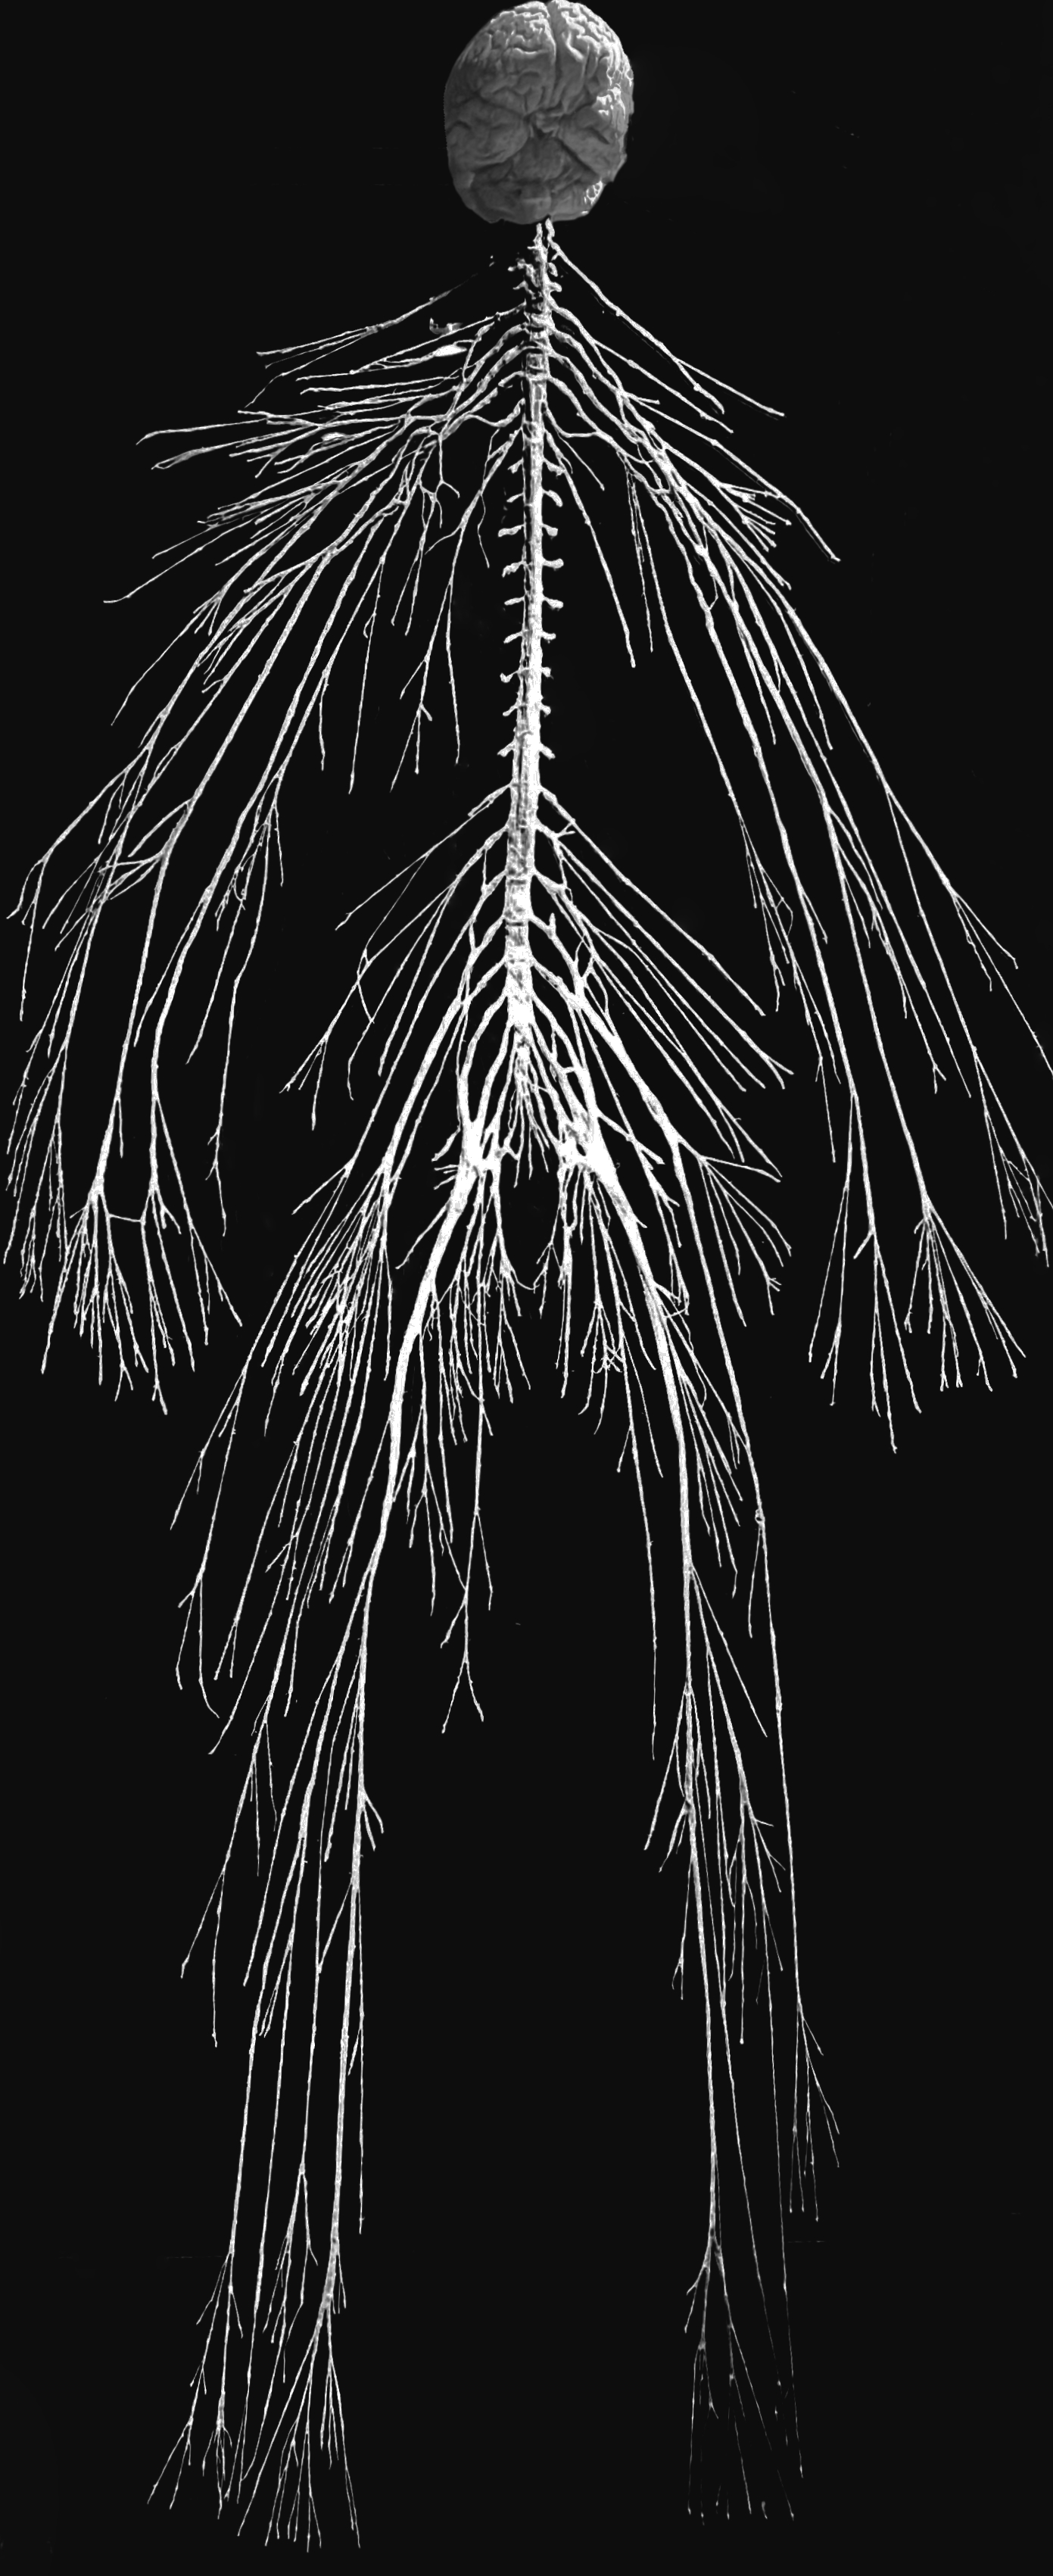
\includegraphics[width=0.7\linewidth]{./figures/nervoussystem/NervousSystem} 

}

\caption{The human nervous system.}\label{fig:nervoussystem}
\end{figure}

The nervous system derives its name from nerves, which are cylindrical bundles of fibers (the axons of neurons), that emanate from the brain and spinal cord, and branch repeatedly to innervate every part of the body. Nerves are large enough to have been recognized by the ancient Egyptians, Greeks, and Romans, but their internal structure was not understood until it became possible to examine them using a microscope.



\begin{figure}

{\centering 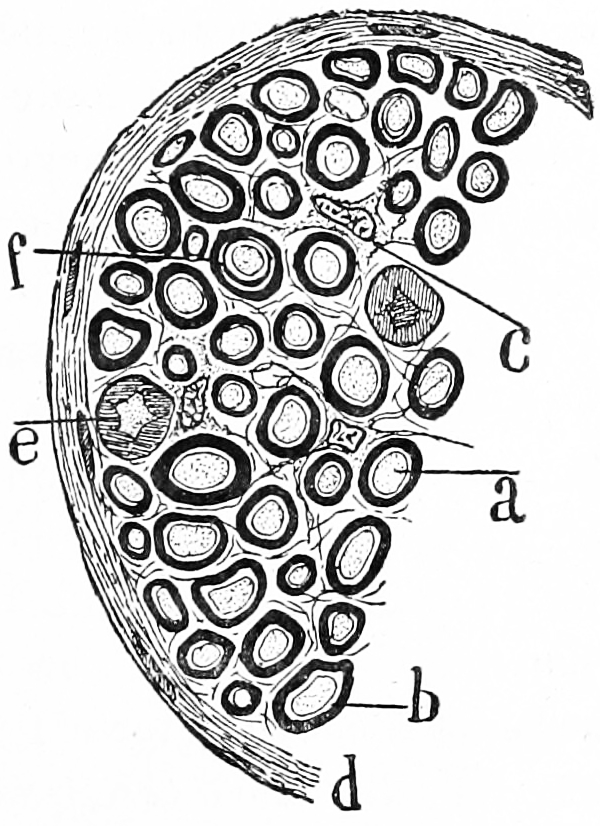
\includegraphics[width=0.7\linewidth]{./figures/nervoussystem/CajalNerve} 

}

\caption{Transverse section of a nerve. a) a single nerve fibre (axon) surrounded by a thick layer of myelin. c) an interstitial cell. \href{https://wellcomelibrary.org/item/b2129592x\#?c=0\&m=0\&s=0\&cv=14\&z=0\%2C-3.48\%2C1\%2C8.6591}{Histologie du système nerveux de l'homme \& des vertébrés, Tome Premier} (1909) by Santiago Ramón y Cajal translated from Spanish by Dr.~L. Azoulay.}\label{fig:nervesection}
\end{figure}



\begin{figure}

{\centering 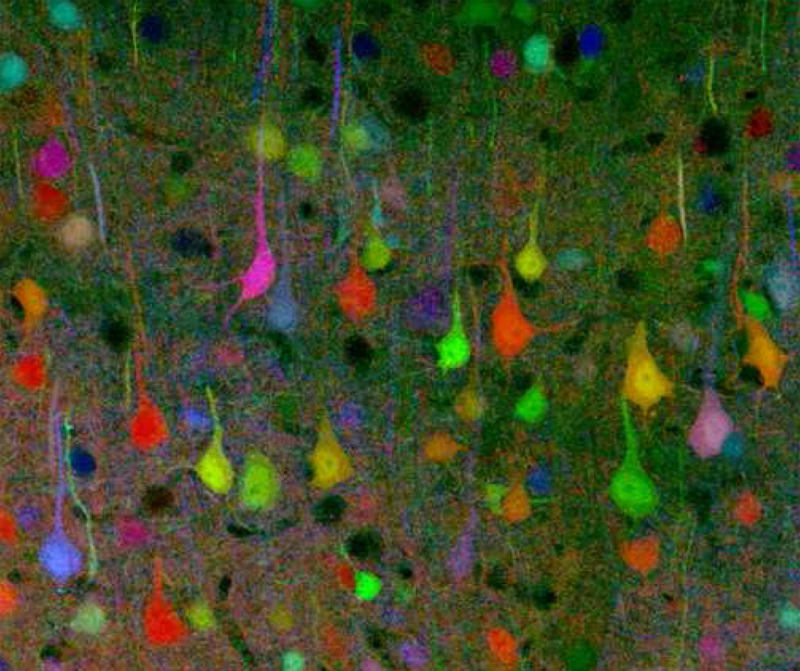
\includegraphics[width=0.7\linewidth]{./figures/nervoussystem/nihms37882f2} 

}

\caption{\href{https://commons.wikimedia.org/wiki/File:Brainbow_(Smith_2007).jpg}{A brainbow of mouse neurons.}}\label{fig:brainbow}
\end{figure}

Neuroscience (or neurobiology) is a multidisciplinary branch of biology that combines physiology, anatomy, molecular biology, developmental biology, cytology, mathematical modeling, and psychology to understand the fundamental and emergent properties of neurons and neural circuits. The understanding of the biological basis of learning, memory, behavior, perception, and consciousness has been described as the ``ultimate challenge'' of the biological sciences. The human brain is often referred to as the most complicated structure in the universe. The scope of neuroscience has broadened over time to include different approaches used to study the nervous system at different scales and the techniques used by neuroscientists have expanded enormously, from molecular and cellular studies of individual neurons to imaging of sensory, motor and cognitive tasks in the brain. Malfunction of the nervous system can occur as a result of genetic defects, physical damage due to trauma or toxicity, infection or simply of ageing. The medical specialty of neurology studies disorders of the nervous system and looks for interventions that can prevent or treat them. Although mental illnesses are believed by many to be neurological disorders affecting the central nervous system, traditionally they are classified separately, and treated by psychiatrists.

Nervous systems are found in most multicellular animals, but vary greatly in complexity. The only multicellular animals that have no nervous system at all are sponges, placozoans, and mesozoans, which have very simple body plans. However, even sponges, unicellular animals, and even protists such as slime molds have cell-to-cell signalling mechanisms that are precursors to those of neurons. The nervous systems of the radially symmetric organisms ctenophores (comb jellies) and cnidarians (which include anemones, hydras, corals and jellyfish) consist of a diffuse nerve net. All other animal species, with the exception of a few types of worm, have a nervous system containing a brain, a central cord (or two cords running in parallel), and nerves radiating from the brain and central cord. The size of the nervous system ranges from a few hundred cells in the simplest worms, to around 300 billion cells in African elephants.

Nervous tissue first arose in wormlike organisms about 550 to 600 million years ago. In humans and other vertebrates it consists of two main parts, the central nervous system (CNS) and the peripheral nervous system (PNS). The CNS consists of the brain and spinal cord. The PNS consists mainly of nerves, which are enclosed bundles of the long fibers or axons, that connect the CNS to every other part of the body. Nerves that transmit signals from the brain are called motor or efferent nerves, while those nerves that transmit information from the body to the CNS are called sensory or afferent. Spinal nerves serve both functions and are called mixed nerves. The PNS is divided into three separate subsystems, the somatic, autonomic, and enteric nervous systems. Somatic nerves carry sensory information from the periphery to the CNS and signals for voluntary movement from the CNS to the muscles. The autonomic nervous system is further subdivided into the sympathetic and the parasympathetic nervous systems. The sympathetic nervous system is activated in cases of emergencies to mobilize energy, while the parasympathetic nervous system is activated when organisms are in a relaxed state. The enteric nervous system functions to control the gastrointestinal system. Both autonomic and enteric nervous systems function involuntarily. Nerves that exit from the cranium are called cranial nerves while those exiting from the spinal cord are called spinal nerves.

\hypertarget{the-cells-of-the-nervous-system}{%
\section{The Cells Of The Nervous System}\label{the-cells-of-the-nervous-system}}

At the cellular level, the nervous system is defined by the presence of a special type of cell, called the neuron, also known as a nerve cell. Neurons have special structures that allow them to receive and send signals from and to other cells. They send these signals in the form of electrochemical waves traveling along thin fibers called axons, which cause chemicals called neurotransmitters to be released at junctions called synapses. Neurons usually receive signalls at tree-like processes called dendrites. A cell that receives a synaptic signal from another neuron may be excited, inhibited, or otherwise modulated. The connections between neurons can form neural pathways, neural circuits, and larger networks that generate an organism's perception of the world and determine its behavior. Along with neurons, the nervous system contains other specialized cells called glial cells (or simply glia), which provide structural and metabolic support.



\begin{figure}

{\centering 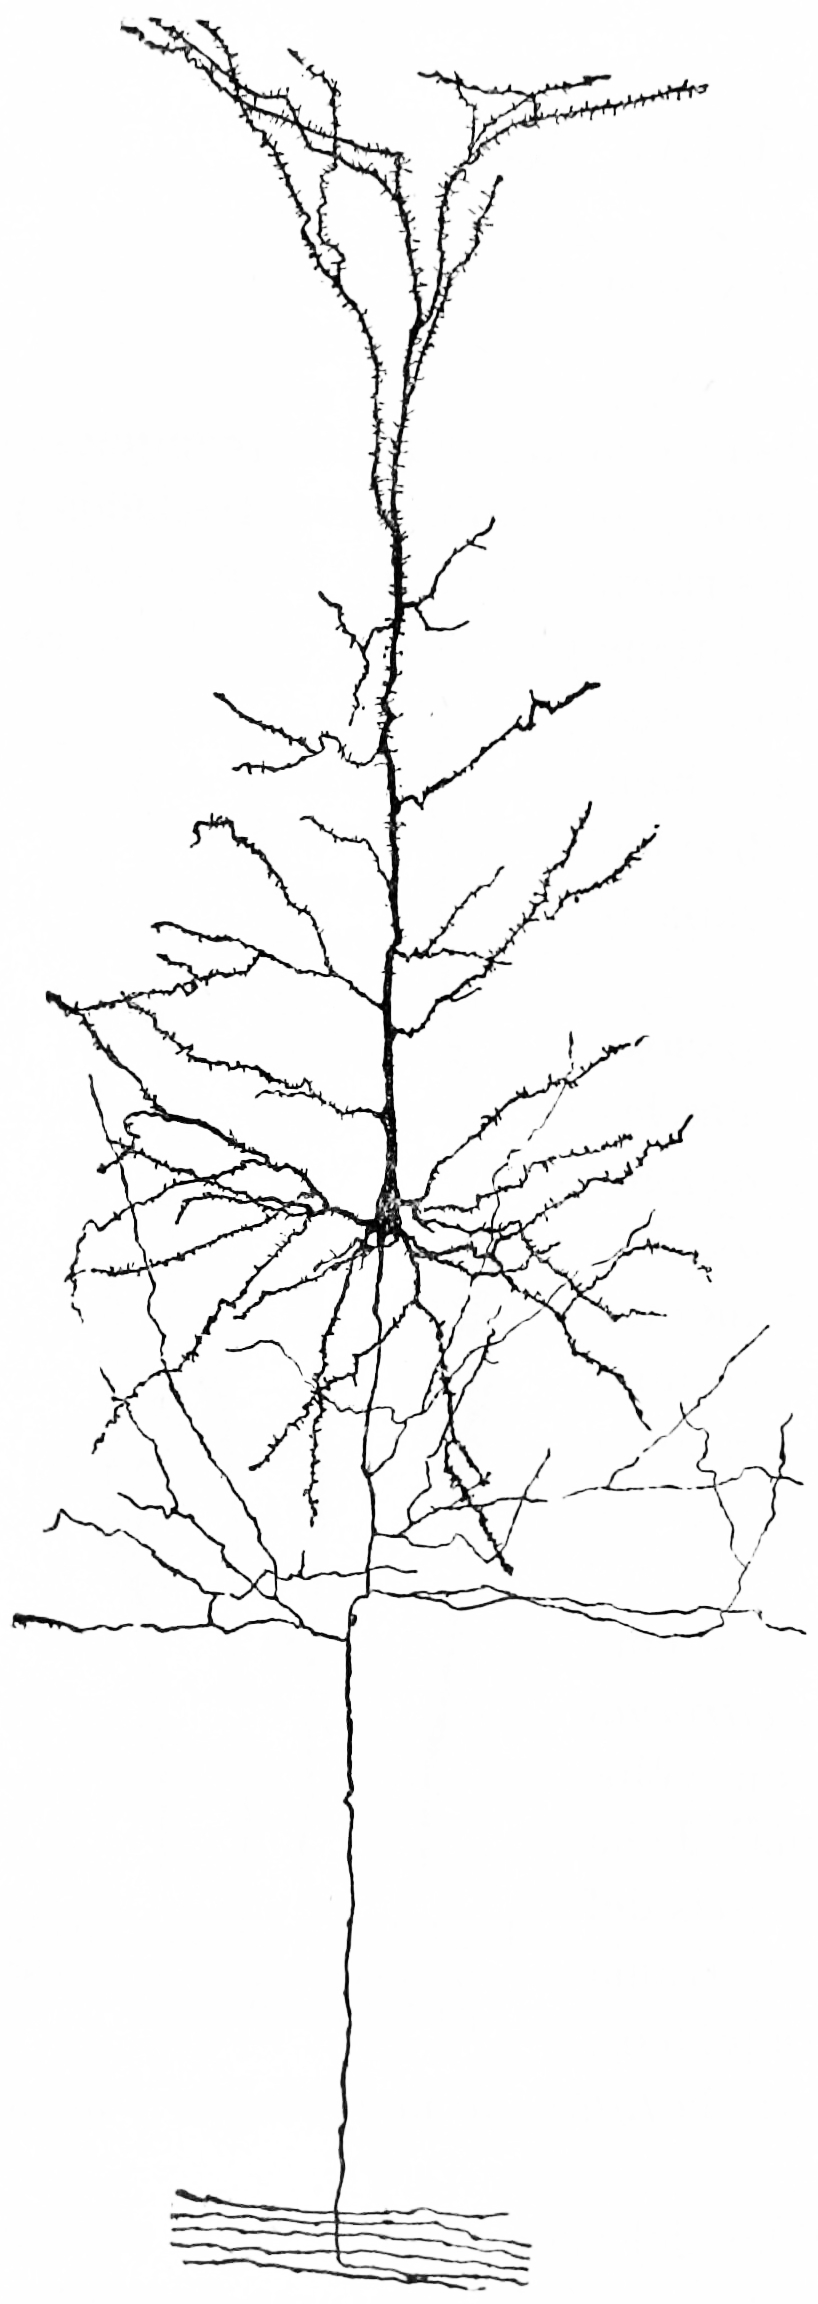
\includegraphics[width=0.7\linewidth]{./figures/nervoussystem/RabbitPyramidalCellCajalMetodos} 

}

\caption{A nerve cell from the cerebral cortex of a rabbit. Notice the extensive tree of dendrites at the top, the long axon at the bottom. Because of the pyramid-like shape of the cell body, this type of neuron is referred to as a pyramidal cell.}\label{fig:pyramidalcell}
\end{figure}

Even in the nervous system of a single species such as humans, hundreds of different types of neurons exist, with a wide variety of morphologies and functions. These include sensory neurons that convert physical stimuli such as light and sound into neural signals, and motor neurons that activate muscles or glands; however in many species the great majority of neurons participate in the formation of centralized structures (the brain and ganglia) and they receive all of their input from other neurons and send their output to other neurons.

Glial cells (named from the Greek for ``glue'') are non-neuronal cells that provide support and nutrition, maintain homeostasis, form myelin, and participate in signal transmission in the nervous system. In the human brain, it is estimated that the total number of glia roughly equals the number of neurons, although the proportions vary in different brain areas. Among the most important functions of glial cells are to support neurons and hold them in place; to supply nutrients to neurons; to insulate neurons electrically; to destroy pathogens and remove dead neurons; and to provide guidance cues directing the axons of neurons to their targets. A very important type of glial cell (oligodendrocytes in the central nervous system, and Schwann cells in the peripheral nervous system) generates layers of a fatty substance called myelin that wraps around axons and provides electrical insulation which allows them to transmit action potentials much more rapidly and efficiently. Microglia serve as important resident immune cells within the central nervous system.

\hypertarget{comparative-anatomy-and-evolution-of-nervous-systems}{%
\section{Comparative Anatomy And Evolution Of Nervous Systems}\label{comparative-anatomy-and-evolution-of-nervous-systems}}

Porifera (sponges) have no cells connected to each other by synaptic junctions, that is, no neurons, and therefore no nervous system. They do, however, have homologs of many genes that play key roles in synaptic function. Recent studies have shown that sponge cells express a group of proteins that cluster together to form a structure resembling a postsynaptic density (the signal-receiving part of a synapse). However, the function of this structure is currently unclear. Although sponge cells do not show synaptic transmission, they do communicate with each other via calcium waves and other impulses, which mediate some simple actions such as whole-body contraction.

Radiata such as the cnidaria (jellyfish) and ctenophora (comb jellies) have diffuse nerve nets rather than a central nervous system. In most jellyfish the nerve net is spread more or less evenly across the body; in comb jellies it is concentrated near the mouth. The nerve nets consist of sensory neurons, which pick up chemical, tactile, and visual signals; motor neurons, which can activate contractions of the body wall; and intermediate neurons, which detect patterns of activity in the sensory neurons and, in response, send signals to groups of motor neurons. In some cases groups of intermediate neurons are clustered into discrete ganglia.

The development of the nervous system in radiata is relatively unstructured. Unlike bilaterians, radiata only have two primordial cell layers, endoderm and ectoderm. Neurons are generated from a special set of ectodermal precursor cells, which also serve as precursors for every other ectodermal cell type.

The vast majority of existing animals are bilaterians, meaning animals with left and right sides that are approximate mirror images of each other. All bilateria are thought to have descended from a common wormlike ancestor that appeared in the Ediacaran period, 550--600 million years ago. The fundamental bilaterian body form is a tube with a hollow gut cavity running from mouth to anus, and a nerve cord with an enlargement (a ``ganglion'') for each body segment, with an especially large ganglion at the front, called the ``brain''.



\begin{figure}

{\centering \includegraphics[width=0.7\linewidth]{./figures/nervoussystem/invertebrate_nervoussystems} 

}

\caption{Comparison of nervous systems of invertebrates. Top left: A diffuse nerve net in \emph{Actinia} (a genus of sea anemones in the family \emph{Actiniidae} in the phylum \emph{Cnidaria}); top right: The nervous system of \emph{Anadonta anatina}, a freshwater mussel in the family \emph{Unionidae} in the phylum \emph{Mollusca}. c, foot; k, pedal ganglion; i, cerebro-pedal connective; g, cerebral ganglion; h, cerebral connective; a, anterior adductor muscle; r, q, anterior pallial nerves; d, liver; s, visceral nerve; l, cerebro-visceral connective; e, gill; f, edge of mantle; n, branchial nerves; m, visceral ganglion; o, posterior pallial nerves; b, posterior adductor muscle; p, lateral pallial nerves; bottom left: the nervous system of \emph{Alitta virens}, a polychaete worm in the phylum \emph{Annelida}. J, jaws; b, antennal nerves; c, palpal nerves; f, ganglia for the dorsal peristomial cirri; n\textsuperscript{1} , ganglion; n, nerves for the dissepimenta; m, parapodial nerves; i, parapodial branch; h, ventral chain of ganglia; C, cerebral ganglion; o, nerve passing through dissepiment to preceding segment; k, parapodial ganglion. Bottom right: the nervous system of an insect (\emph{Arthropoda}). From \href{https://www.biodiversitylibrary.org/ia/morphologyofinve00petr\#page/7/mode/1up}{Morphology of invertebrate types, by Alexander Petrunkevitch. New York, Macmillan company, 1916.}}\label{fig:invertebratenervoussystem}
\end{figure}

Even mammals, including humans, show the segmented bilaterian body plan at the level of the nervous system. The spinal cord contains a series of segmental ganglia, each giving rise to motor and sensory nerves that innervate a portion of the body surface and underlying musculature. On the limbs, the layout of the innervation pattern is complex, but on the trunk it gives rise to a series of narrow bands. The top three segments belong to the brain, giving rise to the forebrain, midbrain, and hindbrain.

Bilaterians can be divided, based on events that occur very early in embryonic development, into two groups (superphyla) called protostomes and deuterostomes. Deuterostomes include vertebrates as well as echinoderms, hemichordates (mainly acorn worms), and Xenoturbellidans. Protostomes, the more diverse group, include arthropods, molluscs, and numerous types of worms. There is a basic difference between the two groups in the placement of the nervous system within the body: protostomes possess a nerve cord on the ventral (usually bottom) side of the body, whereas in deuterostomes the nerve cord is on the dorsal (usually top) side. In fact, numerous aspects of the body are inverted between the two groups, including the expression patterns of several genes that show dorsal-to-ventral gradients. Most anatomists now consider that the bodies of protostomes and deuterostomes are ``flipped over'' with respect to each other, a hypothesis that was first proposed by Geoffroy Saint-Hilaire for insects in comparison to vertebrates. Thus insects, for example, have nerve cords that run along the ventral midline of the body, while all vertebrates have spinal cords that run along the dorsal midline.

There are a few types of existing bilaterians that lack a recognizable brain, including echinoderms and tunicates. It has not been definitively established whether the existence of these brainless species indicates that the earliest bilaterians lacked a brain, or whether their ancestors evolved in a way that led to the disappearance of a previously existing brain structure.

The diversity of invertebrate body plans is matched by an equal diversity in brain structures. Two groups of invertebrates have notably complex brains: arthropods (insects, crustaceans, arachnids, and others), and cephalopods (octopuses, squids, and similar molluscs). The brains of arthropods and cephalopods arise from twin parallel nerve cords that extend through the body of the animal. Arthropods have a central brain, the supraesophageal ganglion, with three divisions and large optical lobes behind each eye for visual processing. Cephalopods such as the octopus and squid have the largest brains of any invertebrates.

There are several invertebrate species whose brains have been studied intensively because they have properties that make them convenient for experimental work:

\begin{itemize}
\tightlist
\item
  Fruit flies (\emph{Drosophila melanogaster}), because of the large array of techniques available for studying their genetics, have been a natural subject for studying the role of genes in brain development. In spite of the large evolutionary distance between insects and mammals, many aspects of \emph{Drosophila} neurogenetics have been shown to be relevant to humans. The first biological clock genes, for example, were identified by examining \emph{Drosophila} mutants that showed disrupted daily activity cycles. A search in the genomes of vertebrates revealed a set of analogous genes, which were found to play similar roles in the mouse biological clock---and therefore almost certainly in the human biological clock as well. Studies done on Drosophila, also show that most neuropil regions of the brain are continuously reorganized throughout life in response to specific living conditions.
\item
  The nematode worm \emph{Caenorhabditis elegans}, like Drosophila, has been studied largely because of its importance in genetics. In the early 1970s, \href{https://en.wikipedia.org/wiki/Sydney_Brenner}{Sydney Brenner} chose it as a model organism for studying the way that genes control development. One of the advantages of working with this worm is that the body plan is very stereotyped: the nervous system of the hermaphrodite contains exactly 302 neurons, always in the same places, making identical synaptic connections in every worm. Brenner's team sliced worms into thousands of ultrathin sections and photographed each one under an electron microscope, then visually matched fibers from section to section, to map out every neuron and synapse in the entire body. The complete neuronal wiring diagram of \emph{C. elegans} -- its connectome was achieved. Nothing approaching this level of detail is available for any other organism, and the information gained has enabled a multitude of studies that would otherwise have not been possible.
\item
  The sea slug \emph{Aplysia californica} was chosen by Nobel Prize-winning neurophysiologist \href{https://en.wikipedia.org/wiki/Eric_Kandel}{Eric Kandel} as a model for studying the cellular basis of learning and memory, because of the simplicity and accessibility of its nervous system, and it has been examined in hundreds of experiments.
\end{itemize}

Worms are the simplest bilaterian animals, and reveal the basic structure of the bilaterian nervous system in the most straightforward way. As an example, earthworms have dual nerve cords running along the length of the body and merging at the tail and the mouth. These nerve cords are connected by transverse nerves like the rungs of a ladder. These transverse nerves help coordinate the two sides of the animal. Two ganglia at the head (the ``nerve ring'') end function similar to a simple brain. Photoreceptors on the animal's eyespots provide sensory information on light and dark.

Arthropods, such as insects and crustaceans, have a nervous system made up of a series of ganglia, connected by a ventral nerve cord made up of two parallel connectives running along the length of the belly. Typically, each body segment has one ganglion on each side, though some ganglia are fused to form the brain and other large ganglia. The head segment contains the brain, also known as the supraesophageal ganglion. In the insect nervous system, the brain is anatomically divided into the protocerebrum, deutocerebrum, and tritocerebrum. Immediately behind the brain is the subesophageal ganglion, which is composed of three pairs of fused ganglia. It controls the mouthparts, the salivary glands and certain muscles. Many arthropods have well-developed sensory organs, including compound eyes for vision and antennae for olfaction and pheromone sensation. The sensory information from these organs is processed by the brain.

In insects, many neurons have cell bodies that are positioned at the edge of the brain and are electrically passive---the cell bodies serve only to provide metabolic support and do not participate in signalling. A protoplasmic fiber runs from the cell body and branches profusely, with some parts transmitting signals and other parts receiving signals. Thus, most parts of the insect brain have passive cell bodies arranged around the periphery, while the neural signal processing takes place in a tangle of protoplasmic fibers called neuropil, in the interior.

Brains are most simply compared in terms of their size. The relationship between brain size, body size and other variables has been studied across a wide range of vertebrate species. As a rule, brain size increases with body size, but not in a simple linear proportion. In general, smaller animals tend to have larger brains, measured as a fraction of body size. For mammals, the relationship between brain volume and body mass essentially follows a power law with an exponent of about 0.75. This formula describes the central tendency, but every family of mammals departs from it to some degree, in a way that reflects in part the complexity of their behavior. For example, primates have brains 5 to 10 times larger than the formula predicts. Predators tend to have larger brains than their prey, relative to body size.

All vertebrate brains share a common underlying form, which appears most clearly during early stages of embryonic development. In its earliest form, the brain appears as three swellings at the front end of the neural tube; these swellings eventually become the forebrain, midbrain, and hindbrain (the prosencephalon, mesencephalon, and rhombencephalon, respectively). At the earliest stages of brain development, the three areas are roughly equal in size. In many classes of vertebrates, such as fish and amphibians, the three parts remain similar in size in the adult, but in mammals the forebrain becomes much larger than the other parts, and the midbrain becomes very small.



\begin{figure}

{\centering 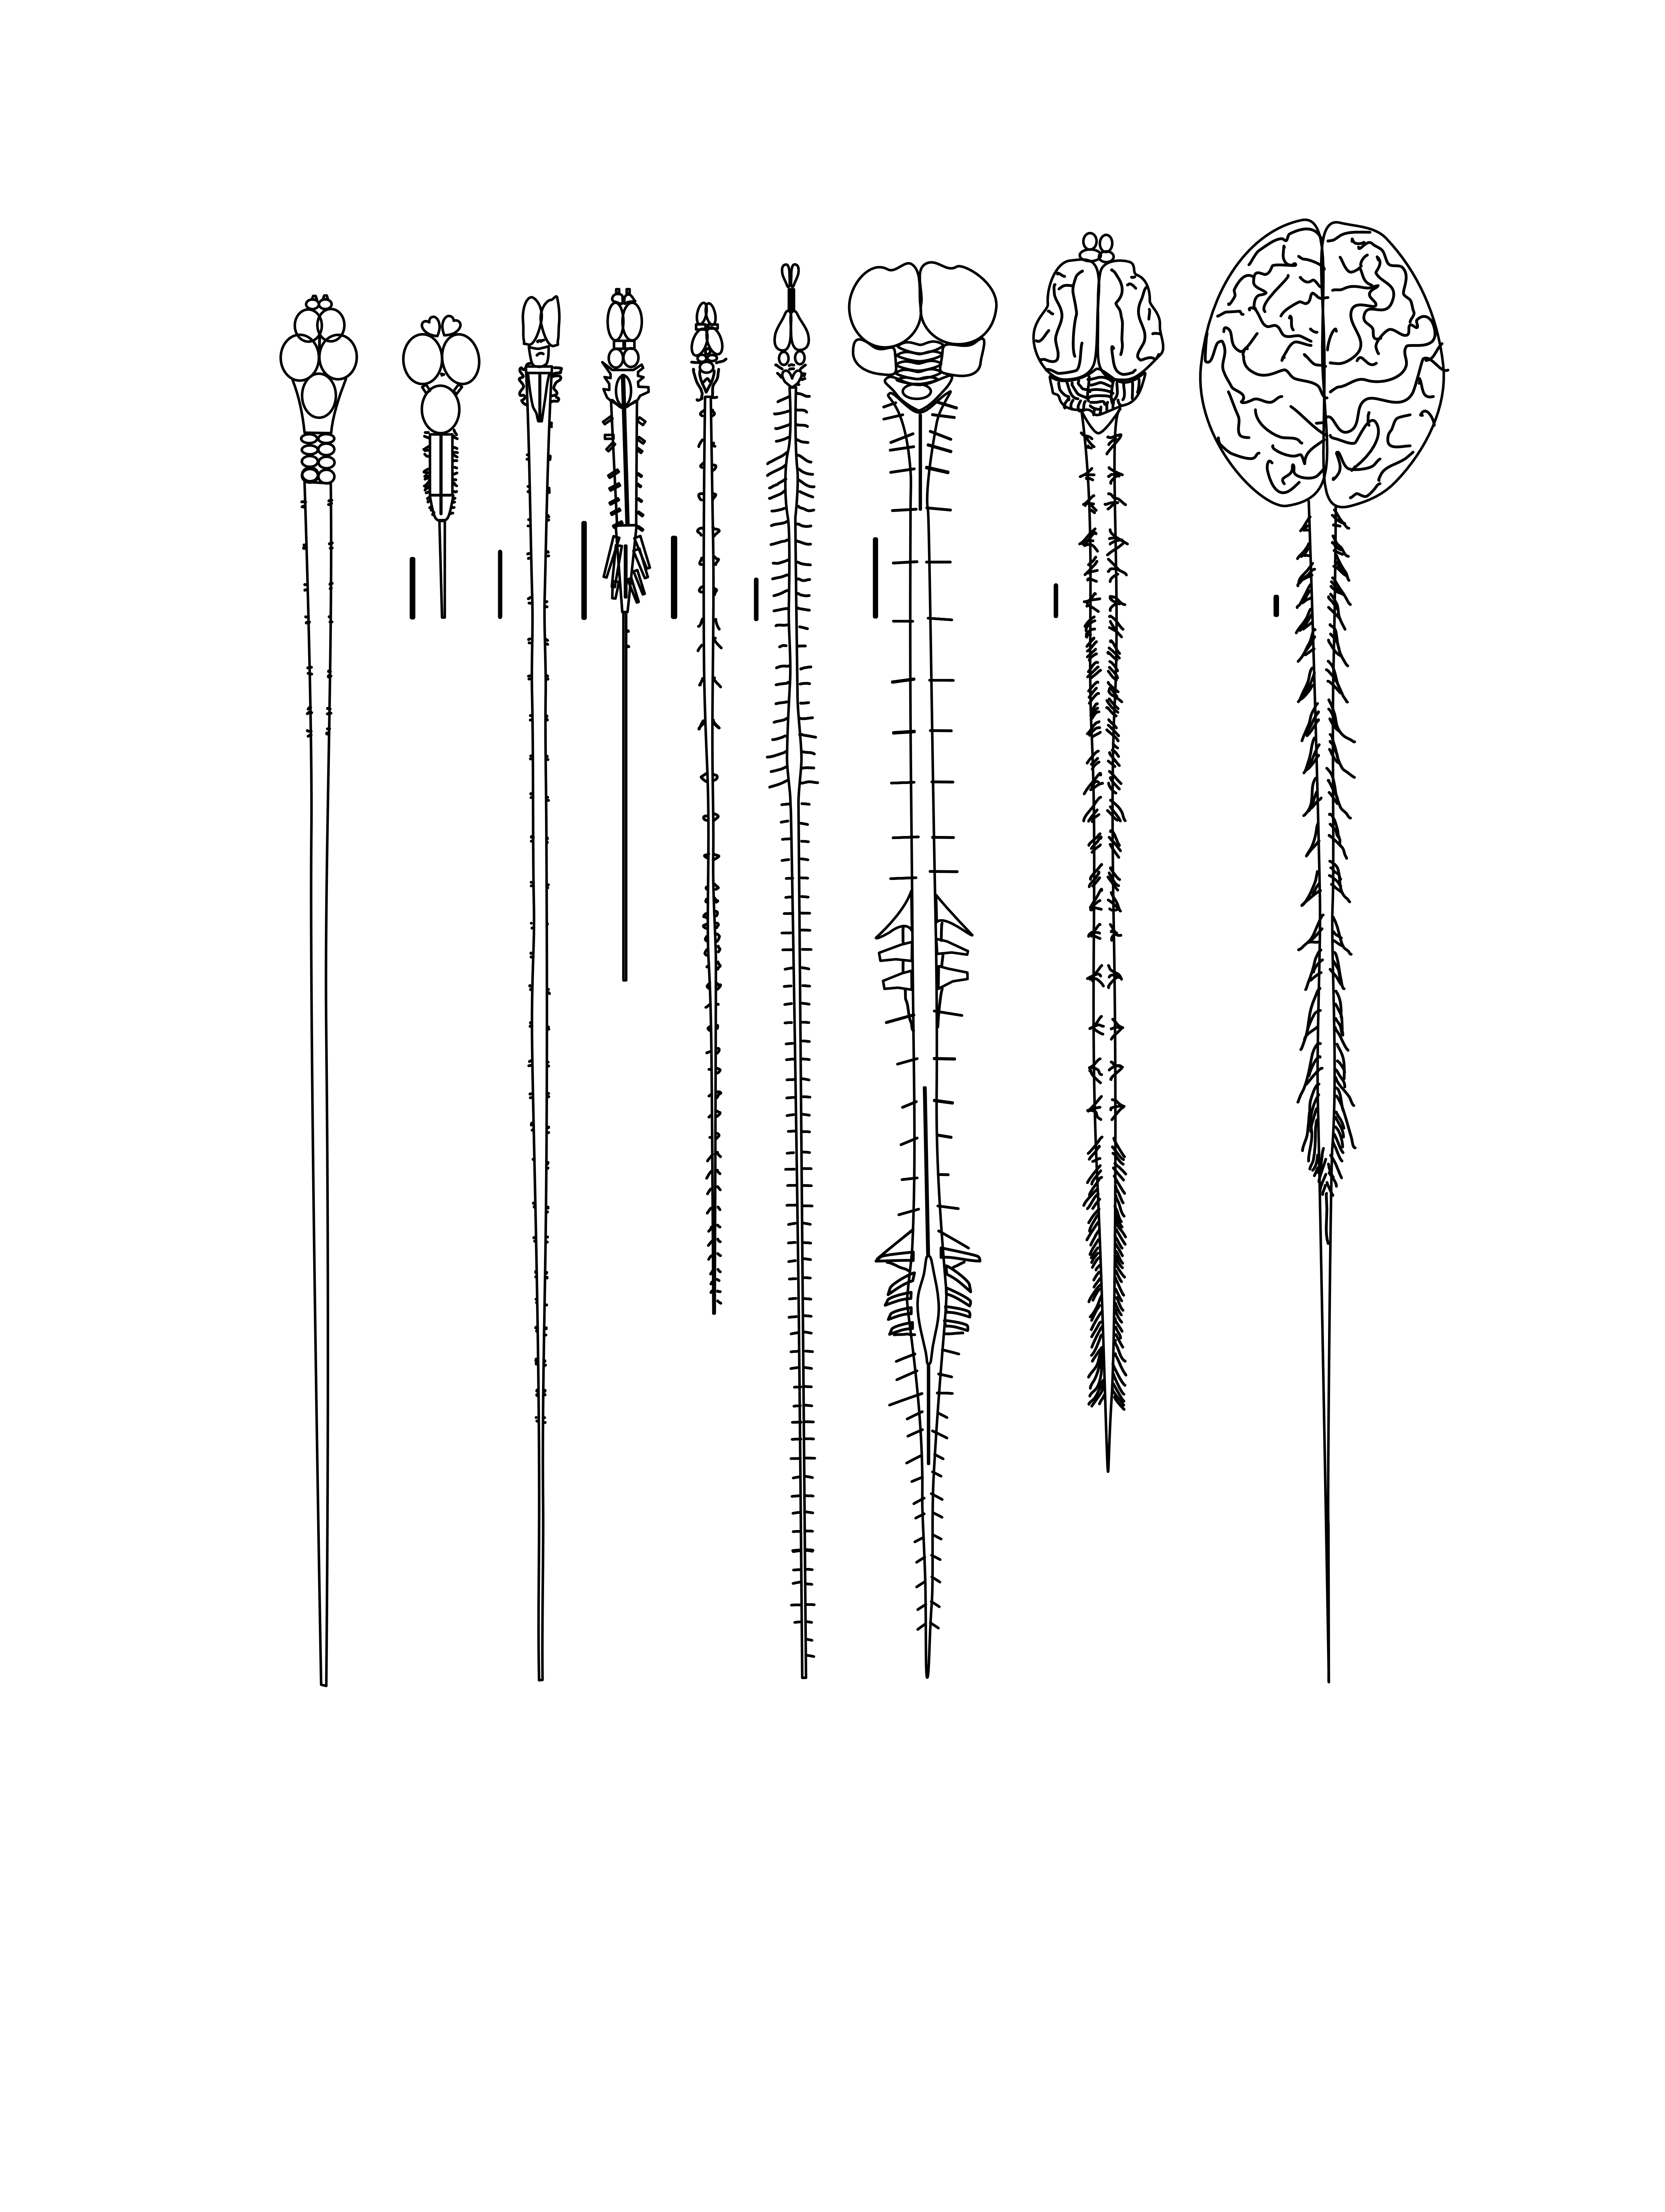
\includegraphics[width=0.7\linewidth]{./figures/nervoussystem/cns_comparison} 

}

\caption{Dorsal views of the central nervous systems of the teleosts (from left to right) \emph{Trigla hirundo} (a) and \emph{Mola mola}, the urodele \emph{Ambystoma tigrinum}, the anuran \emph{Xenopus laevis}, the tortoise \emph{Testudo hermanni}, the tegu lizard \emph{Tupinambis teguixin}, the pigeon, the cat and human. In a, c, d, e, f, g and j the full length of the spinalcord, including the filum terminale (where present) is shown; in \emph{Mola mola} and the cat most of the filum terminale is cut. Vertical black bars correspond to 1 cm in length. Modified from \href{https://doi.org/10.1007/978-3-642-18262-4_24}{Nieuwenhuys, R., ten Donkelaar, H. J., \& Nicholson, C. (1998). The Meaning of It All. The Central Nervous System of Vertebrates, 2135--2195}}\label{fig:vertebratecns}
\end{figure}

The brains of vertebrates are made of very soft tissue. Living brain tissue is pinkish on the outside and mostly white on the inside, with subtle variations in color. Vertebrate brains are surrounded by a system of connective tissue membranes called meninges that separate the skull from the brain. Blood vessels enter the central nervous system through holes in the meningeal layers. The cells in the blood vessel walls are joined tightly to one another, forming the blood--brain barrier, which blocks the passage of many toxins and pathogens (though at the same time blocking antibodies and some drugs, thereby presenting special challenges in treatment of diseases of the brain).

Neuroanatomists usually divide the vertebrate brain into six main regions: the telencephalon (cerebral hemispheres), diencephalon (thalamus and hypothalamus), mesencephalon (midbrain), cerebellum, pons, and medulla oblongata. Each of these areas has a complex internal structure. Some parts, such as the cerebral cortex and the cerebellar cortex, consist of layers that are folded or convoluted to fit within the available space. Other parts, such as the thalamus and hypothalamus, consist of clusters of many small nuclei. Thousands of distinguishable areas can be identified within the vertebrate brain based on fine distinctions of neural structure, chemistry, and connectivity.

There is an anatomical convention that a cluster of neurons in the brain or spinal cord is called a nucleus, whereas a cluster of neurons in the periphery is called a ganglion. There are, however, a few exceptions to this rule, notably including the part of the forebrain called the basal ganglia.

Although the same basic components are present in all vertebrate brains, some branches of vertebrate evolution have led to substantial distortions of brain geometry, especially in the forebrain area. The brain of a shark shows the basic components in a straightforward way, but in teleost fishes (the great majority of existing fish species), the forebrain has become ``everted'', like a sock turned inside out. In birds, there are also major changes in forebrain structure. These distortions can make it difficult to match brain components from one species with those of another species.

Here is a list of some of the most important vertebrate brain components, along with a brief description of their functions as currently understood:

\begin{itemize}
\tightlist
\item
  The medulla, along with the spinal cord, contains many small nuclei involved in a wide variety of sensory and involuntary motor functions such as vomiting, heart rate and digestive processes.
\item
  The pons lies in the brainstem directly above the medulla. Among other things, it contains nuclei that control often voluntary but simple acts such as sleep, respiration, swallowing, bladder function, equilibrium, eye movement, facial expressions, and posture.
\item
  The hypothalamus is a small region at the base of the forebrain, whose complexity and importance belies its size. It is composed of numerous small nuclei, each with distinct connections and neurochemistry. The hypothalamus is engaged in additional involuntary or partially voluntary acts such as sleep and wake cycles, eating and drinking, and the release of some hormones.
\item
  The thalamus is a collection of nuclei with diverse functions: some are involved in relaying information to and from the cerebral hemispheres, while others are involved in motivation. The subthalamic area (zona incerta) seems to contain action-generating systems for several types of ``consummatory'' behaviors such as eating, drinking, defecation, and copulation.
\item
  The cerebellum modulates the outputs of other brain systems, whether motor related or thought related, to make them certain and precise. Removal of the cerebellum does not prevent an animal from doing anything in particular, but it makes actions hesitant and clumsy. This precision is not built-in, but learned by trial and error. The muscle coordination learned while riding a bicycle is an example of a type of neural plasticity that may take place largely within the cerebellum. 10\% of the brain's total volume consists of the cerebellum and 50\% of all neurons are held within its structure.
\item
  The optic tectum allows actions to be directed toward points in space, most commonly in response to visual input. In mammals it is usually referred to as the superior colliculus, and its best-studied function is to direct eye movements. It also directs reaching movements and other object-directed actions. It receives strong visual inputs, but also inputs from other senses that are useful in directing actions, such as auditory input in owls and input from the thermosensitive pit organs in snakes. In some primitive fishes, such as lampreys, this region is the largest part of the brain. The superior colliculus is part of the midbrain.
\item
  The pallium is a layer of gray matter that lies on the surface of the forebrain and is the most complex and most recent evolutionary development of the brain as an organ. In reptiles and mammals, it is called the cerebral cortex. Multiple functions involve the pallium, including smell and spatial memory. In mammals, where it becomes so large as to dominate the brain, it takes over functions from many other brain areas. In many mammals, the cerebral cortex consists of folded bulges called gyri that create deep furrows or fissures called sulci. The folds increase the surface area of the cortex and therefore increase the amount of gray matter and the amount of information that can be stored and processed.
\item
  The hippocampus, strictly speaking, is found only in mammals. However, the area it derives from, the medial pallium, has counterparts in all vertebrates. There is evidence that this part of the brain is involved in complex events such as spatial memory and navigation in fishes, birds, reptiles, and mammals.
\item
  The basal ganglia are a group of interconnected structures in the forebrain. The primary function of the basal ganglia appears to be action selection: they send inhibitory signals to all parts of the brain that can generate motor behaviors, and in the right circumstances can release the inhibition, so that the action-generating systems are able to execute their actions. Reward and punishment exert their most important neural effects by altering connections within the basal ganglia.
\item
  The olfactory bulb is a special structure that processes olfactory sensory signals and sends its output to the olfactory part of the pallium. It is a major brain component in many vertebrates, but is greatly reduced in humans and other primates (whose senses are dominated by information acquired by sight rather than smell).
\end{itemize}

The most obvious difference between the brains of mammals and other vertebrates is in terms of size. On average, a mammal has a brain roughly twice as large as that of a bird of the same body size, and ten times as large as that of a reptile of the same body size.

Size, however, is not the only difference: there are also substantial differences in shape. The hindbrain and midbrain of mammals are generally similar to those of other vertebrates, but dramatic differences appear in the forebrain, which is greatly enlarged and also altered in structure. The cerebral cortex is the part of the brain that most strongly distinguishes mammals. In non-mammalian vertebrates, the surface of the cerebrum is lined with a comparatively simple three-layered structure called the pallium. In mammals, the pallium evolves into a complex six-layered structure called neocortex or isocortex. Several areas at the edge of the neocortex, including the hippocampus and amygdala, are also much more extensively developed in mammals than in other vertebrates.

The elaboration of the cerebral cortex carries with it changes to other brain areas. The superior colliculus, which plays a major role in visual control of behavior in most vertebrates, shrinks to a small size in mammals, and many of its functions are taken over by visual areas of the cerebral cortex. The cerebellum of mammals contains a large portion (the neocerebellum) dedicated to supporting the cerebral cortex, which has no counterpart in other vertebrates.

The brains of humans and other primates contain the same structures as the brains of other mammals, but are generally larger in proportion to body size. The encephalization quotient (EQ) is used to compare brain sizes across species. It takes into account the nonlinearity of the brain-to-body relationship. Humans have an average EQ in the 7-to-8 range, while most other primates have an EQ in the 2-to-3 range. Dolphins have values higher than those of primates other than humans, but nearly all other mammals have EQ values that are substantially lower.



\begin{figure}

{\centering 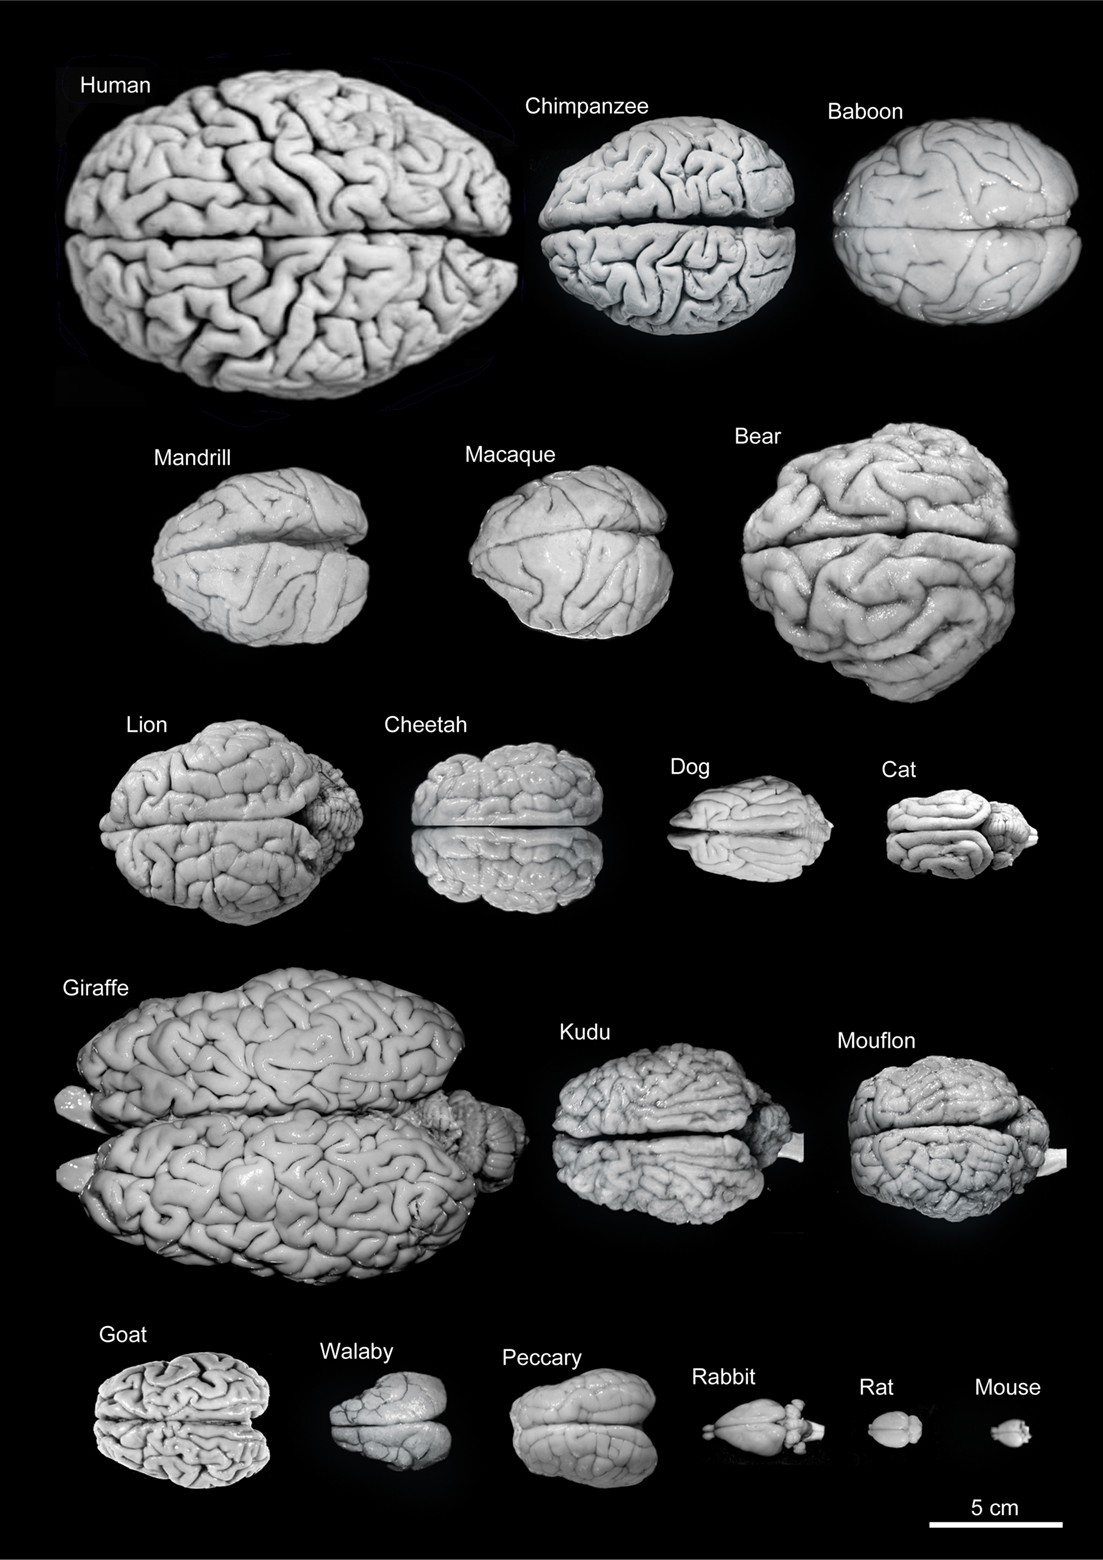
\includegraphics[width=0.7\linewidth]{./figures/nervoussystem/fnana-05-00029-g007} 

}

\caption{Variability of brain size and external topography. Photographs and weights of the brains of different species. Primates: human (Homo sapiens, 1.176 kg), chimpanzee (Pan troglodytes, 273 g), baboon (Papio cynocephalus, 151 g), mandrill (Mandrillus sphinx, 123 g), macaque (Macaca tonkeana, 110 g). Carnivores: bear (Ursus arctos, 289 g), lion (Panthera leo, 165 g), cheetah (Acinonyx jubatus, 119 g), dog (Canis familiaris, 95 g), cat (Felis catus, 32 g). Artiodactyls: giraffe (Giraffa camelopardalis, 700 g), kudu (Tragelaphus strepsiceros, 166 g), mouflon (Ovis musimon, 118 g), ibex (Capra pyrenaica, 115 g); peccary (Tayassu pecari, 41 g). Marsupials: wallaby (Protemnodon rufogrisea, 28 g). Lagomorphs: rabbit (Oryctolagus cuniculus, 5.2 g). Rodents: rat (Rattus rattus, 2.6 g), mouse (Mus musculus, 0.5 g). The chimpanzee brain was kindly supplied by Dr.~Dean Falk. The rest of non-human brains were from material used in Ballesteros-Yánez et al., 2005). Scale bar: 5 cm. From \href{https://www.frontiersin.org/article/10.3389/fnana.2011.00029}{DeFelipe J (2011) The evolution of the brain, the human nature of cortical circuits, and intellectual creativity. Front. Neuroanat. 5:29}}\label{fig:mammaliancns}
\end{figure}

Most of the enlargement of the primate brain comes from a massive expansion of the cerebral cortex, especially the prefrontal cortex and the parts of the cortex involved in vision. The visual processing network of primates includes at least 30 distinguishable brain areas, with a complex web of interconnections. It has been estimated that visual processing areas occupy more than half of the total surface of the primate neocortex. The prefrontal cortex carries out functions that include planning, working memory, motivation, attention, and executive control. It takes up a much larger proportion of the brain for primates than for other species, and an especially large fraction of the human brain.

The peripheral nervous system (PNS) is a collective term for the nervous system structures that do not lie within the CNS. The large majority of the axon bundles called nerves are considered to belong to the PNS, even when the cell bodies of the neurons to which they belong reside within the brain or spinal cord. The PNS is divided into somatic and visceral parts. The somatic part consists of the nerves that innervate the skin, joints, and muscles. The cell bodies of somatic sensory neurons lie in dorsal root ganglia of the spinal cord. The visceral part, also known as the autonomic nervous system, contains neurons that innervate the internal organs, blood vessels, and glands. The autonomic nervous system itself consists of two parts: the sympathetic nervous system and the parasympathetic nervous system. Some authors also include sensory neurons whose cell bodies lie in the periphery (for senses such as hearing) as part of the PNS; others, however, omit them.

The vertebrate nervous system can also be divided into areas called gray matter and white matter. Gray matter (which is only gray in preserved tissue, and is better described as pink or light brown in living tissue) contains a high proportion of cell bodies of neurons. White matter is composed mainly of myelinated axons, and takes its color from the myelin. White matter includes all of the nerves, and much of the interior of the brain and spinal cord. Gray matter is found in clusters of neurons in the brain and spinal cord, and in cortical layers that line their surfaces.

\hypertarget{the-human-brain}{%
\section{The Human Brain}\label{the-human-brain}}

The adult human brain weighs on average about 1.2--1.4 kg (2.6--3.1 lb) which is about 2\% of the total body weight, with a volume of around 1260 cm\textsuperscript{3} in men and 1130 cm\textsuperscript{3} in women. There is substantial individual variation, with the standard reference range for men being 1,180--1,620 g (2.60--3.57 lb) and for women 1,030--1,400 g (2.27--3.09 lb).

The human brain is divided into nearly symmetrical left and right hemispheres by a deep groove, the longitudinal fissure. Each hemisphere is conventionally divided into four main lobes; the frontal lobe, parietal lobe, temporal lobe, and occipital lobe, named according to the skull bones that overlie them. The surface of the brain is folded into ridges (gyri) and grooves (sulci), many of which are named, usually according to their position, such as the frontal gyrus of the frontal lobe or the central sulcus separating the central regions of the hemispheres. There are many small variations in the secondary and tertiary folds.



\begin{figure}

{\centering 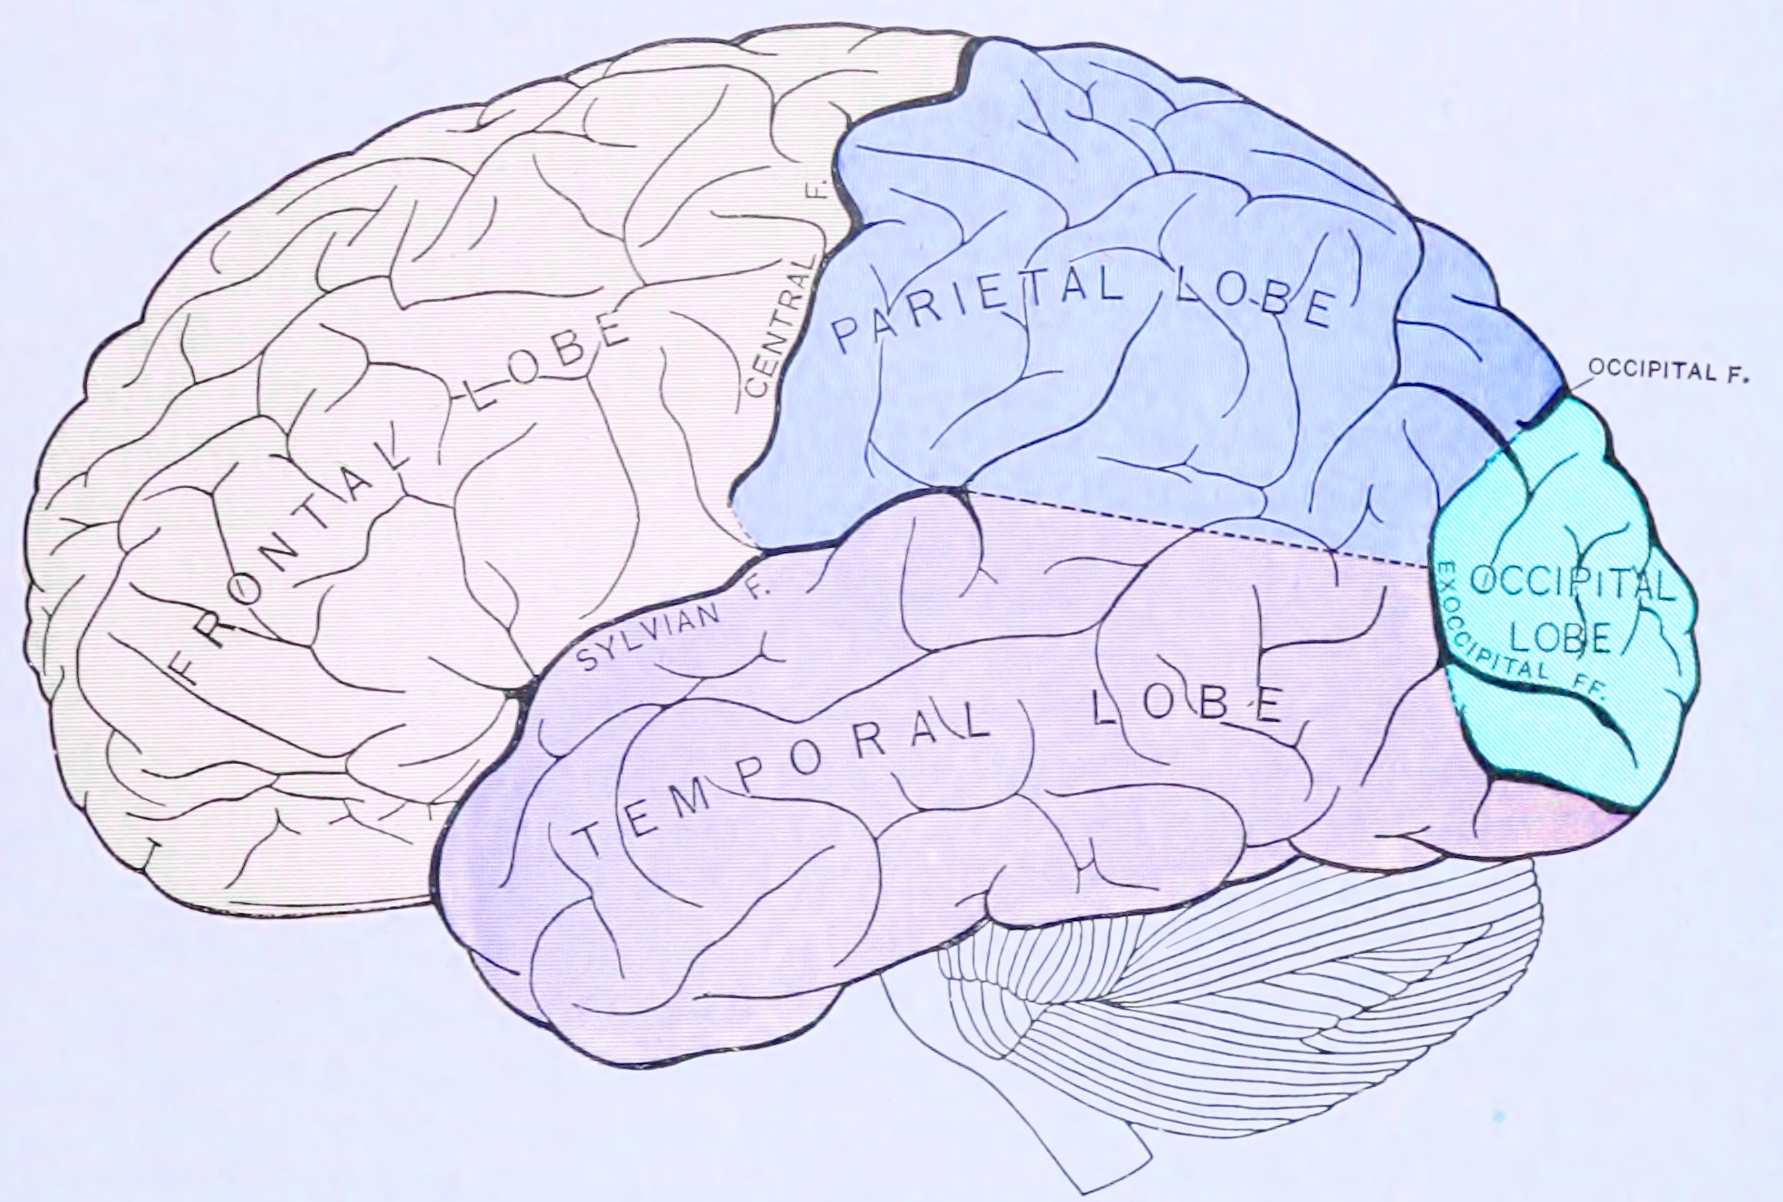
\includegraphics[width=0.7\linewidth]{./figures/nervoussystem/GrayAnat1918p821} 

}

\caption{Principal lobes and fissures of the cerebrum viewed laterally. From \href{https://archive.org/details/anatomyofhumanbo1918gray/page/n6/mode/2up}{Gray Henry, Anatomy of the Human Body. 20\textsuperscript{th} Edition, Lea \& Febiger, Philadelphia \& New York, 1918}}\label{fig:principallobes}
\end{figure}



\begin{figure}

{\centering 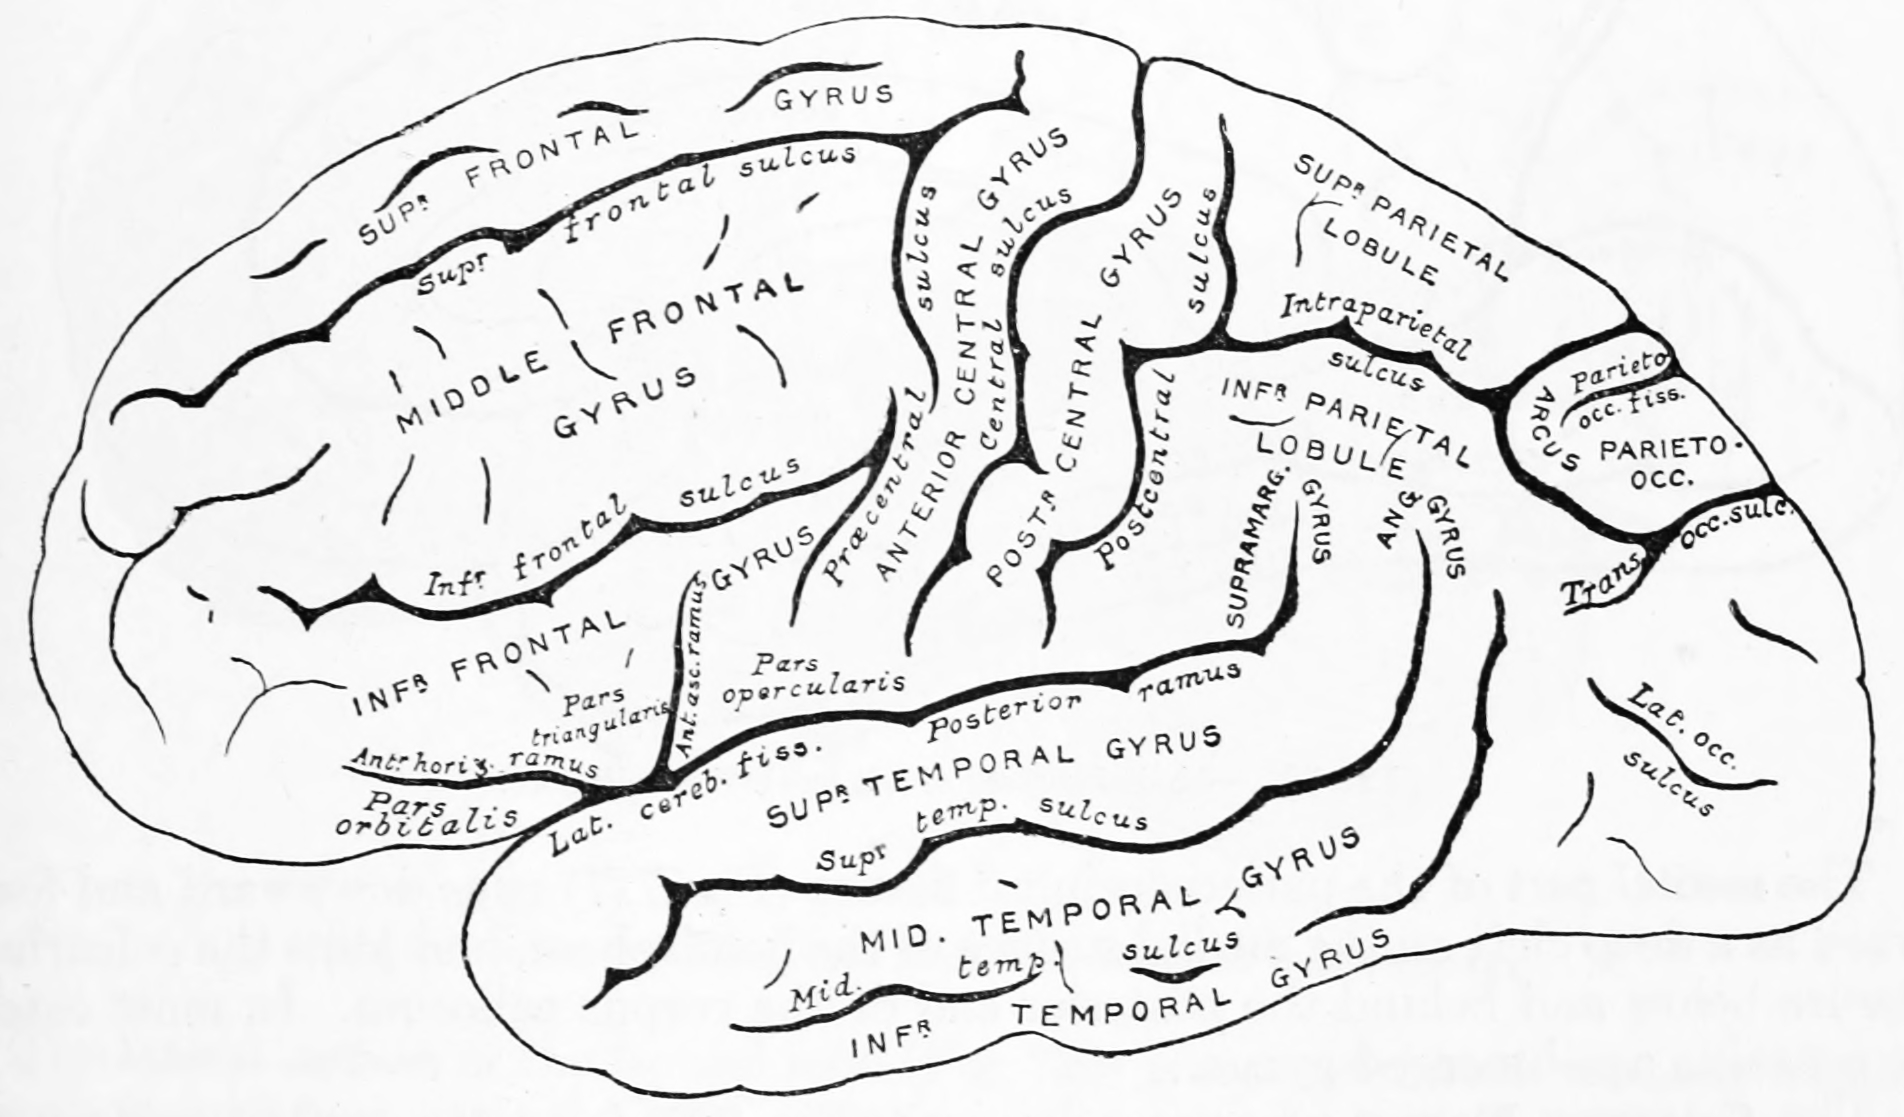
\includegraphics[width=0.7\linewidth]{./figures/nervoussystem/GrayAnat1918p819} 

}

\caption{Diagram showing a lateral view of the ridges (gyri) and grooves (sulci) of the left hemisphere of the brain. From \href{https://archive.org/details/anatomyofhumanbo1918gray/page/n6/mode/2up}{Gray Henry, Anatomy of the Human Body. 20\textsuperscript{th} Edition, Lea \& Febiger, Philadelphia \& New York, 1918}}\label{fig:gyrilateral}
\end{figure}



\begin{figure}

{\centering 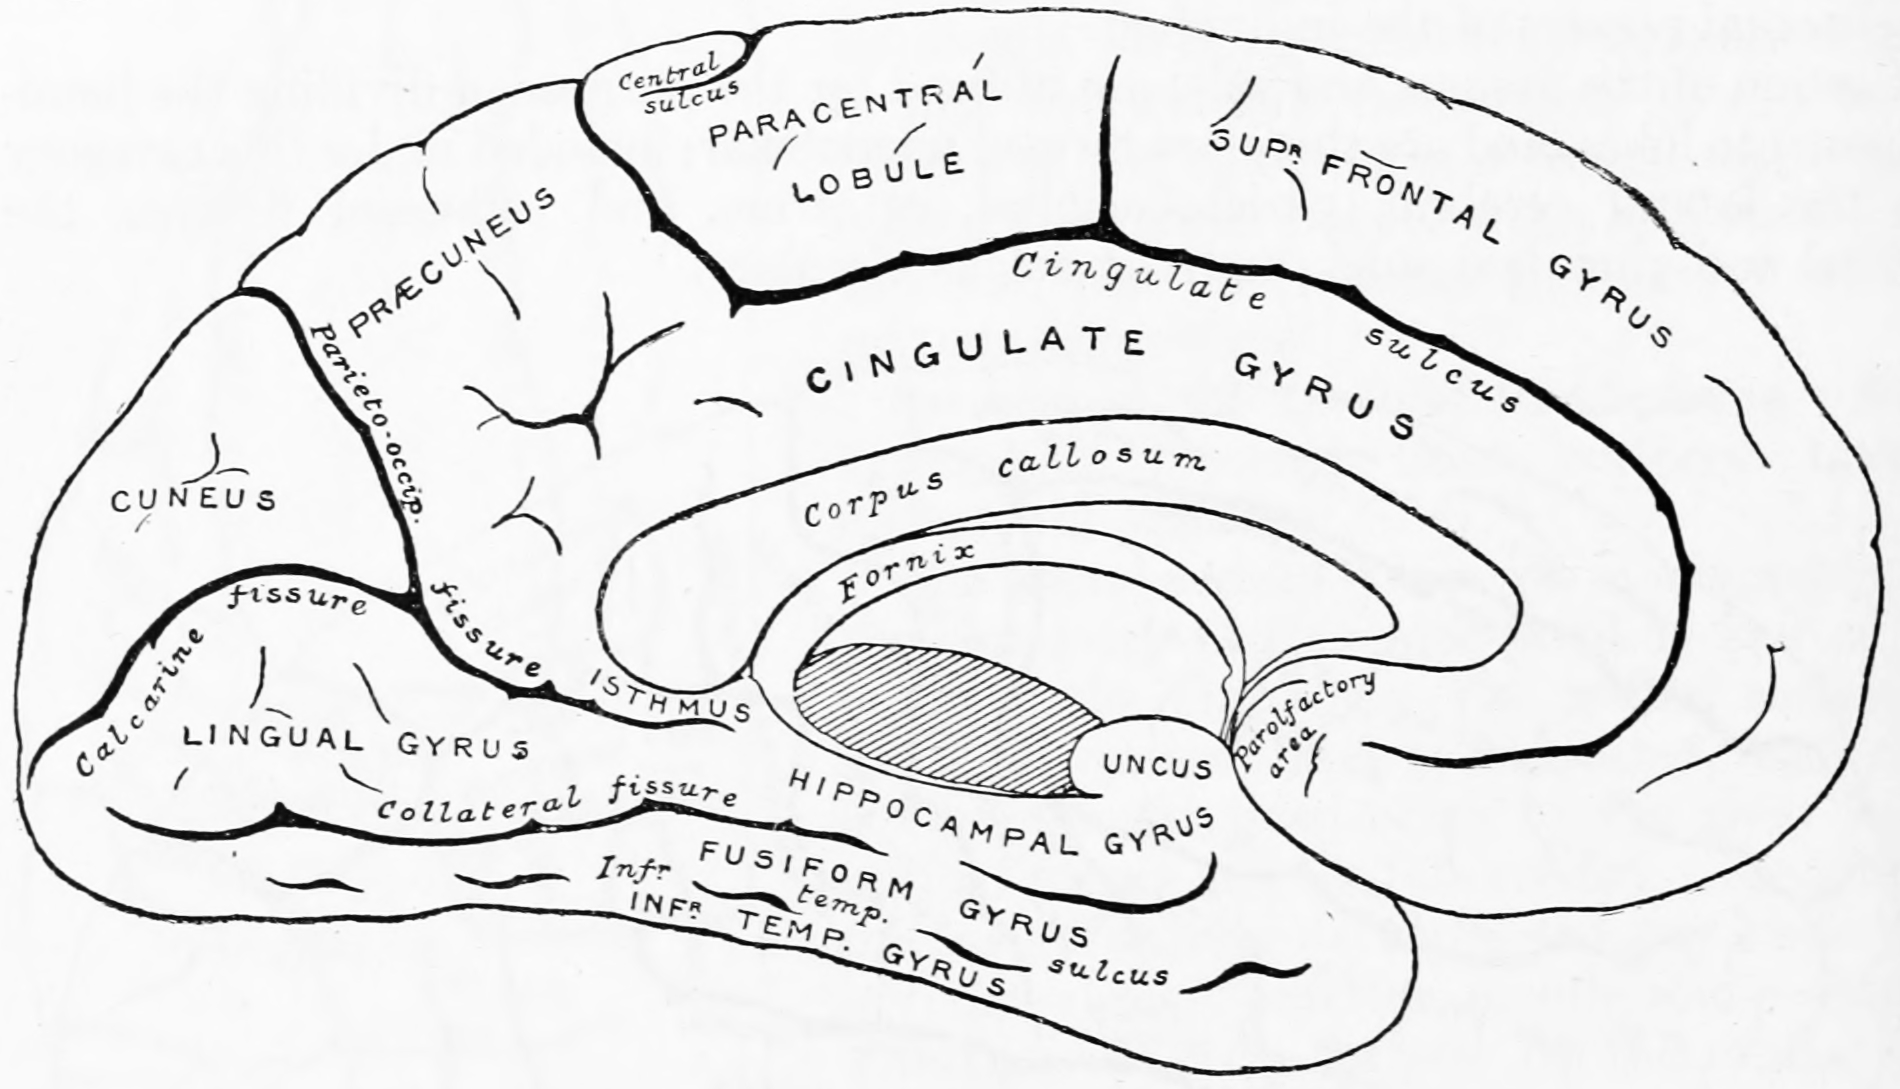
\includegraphics[width=0.7\linewidth]{./figures/nervoussystem/GrayAnat1918p820} 

}

\caption{Diagram showing a medial view of the ridges (gyri) and grooves (sulci) of the left hemisphere of the brain. From \href{https://archive.org/details/anatomyofhumanbo1918gray/page/n6/mode/2up}{Gray Henry, Anatomy of the Human Body. 20\textsuperscript{th} Edition, Lea \& Febiger, Philadelphia \& New York, 1918}}\label{fig:gyrimedial}
\end{figure}



\begin{figure}

{\centering 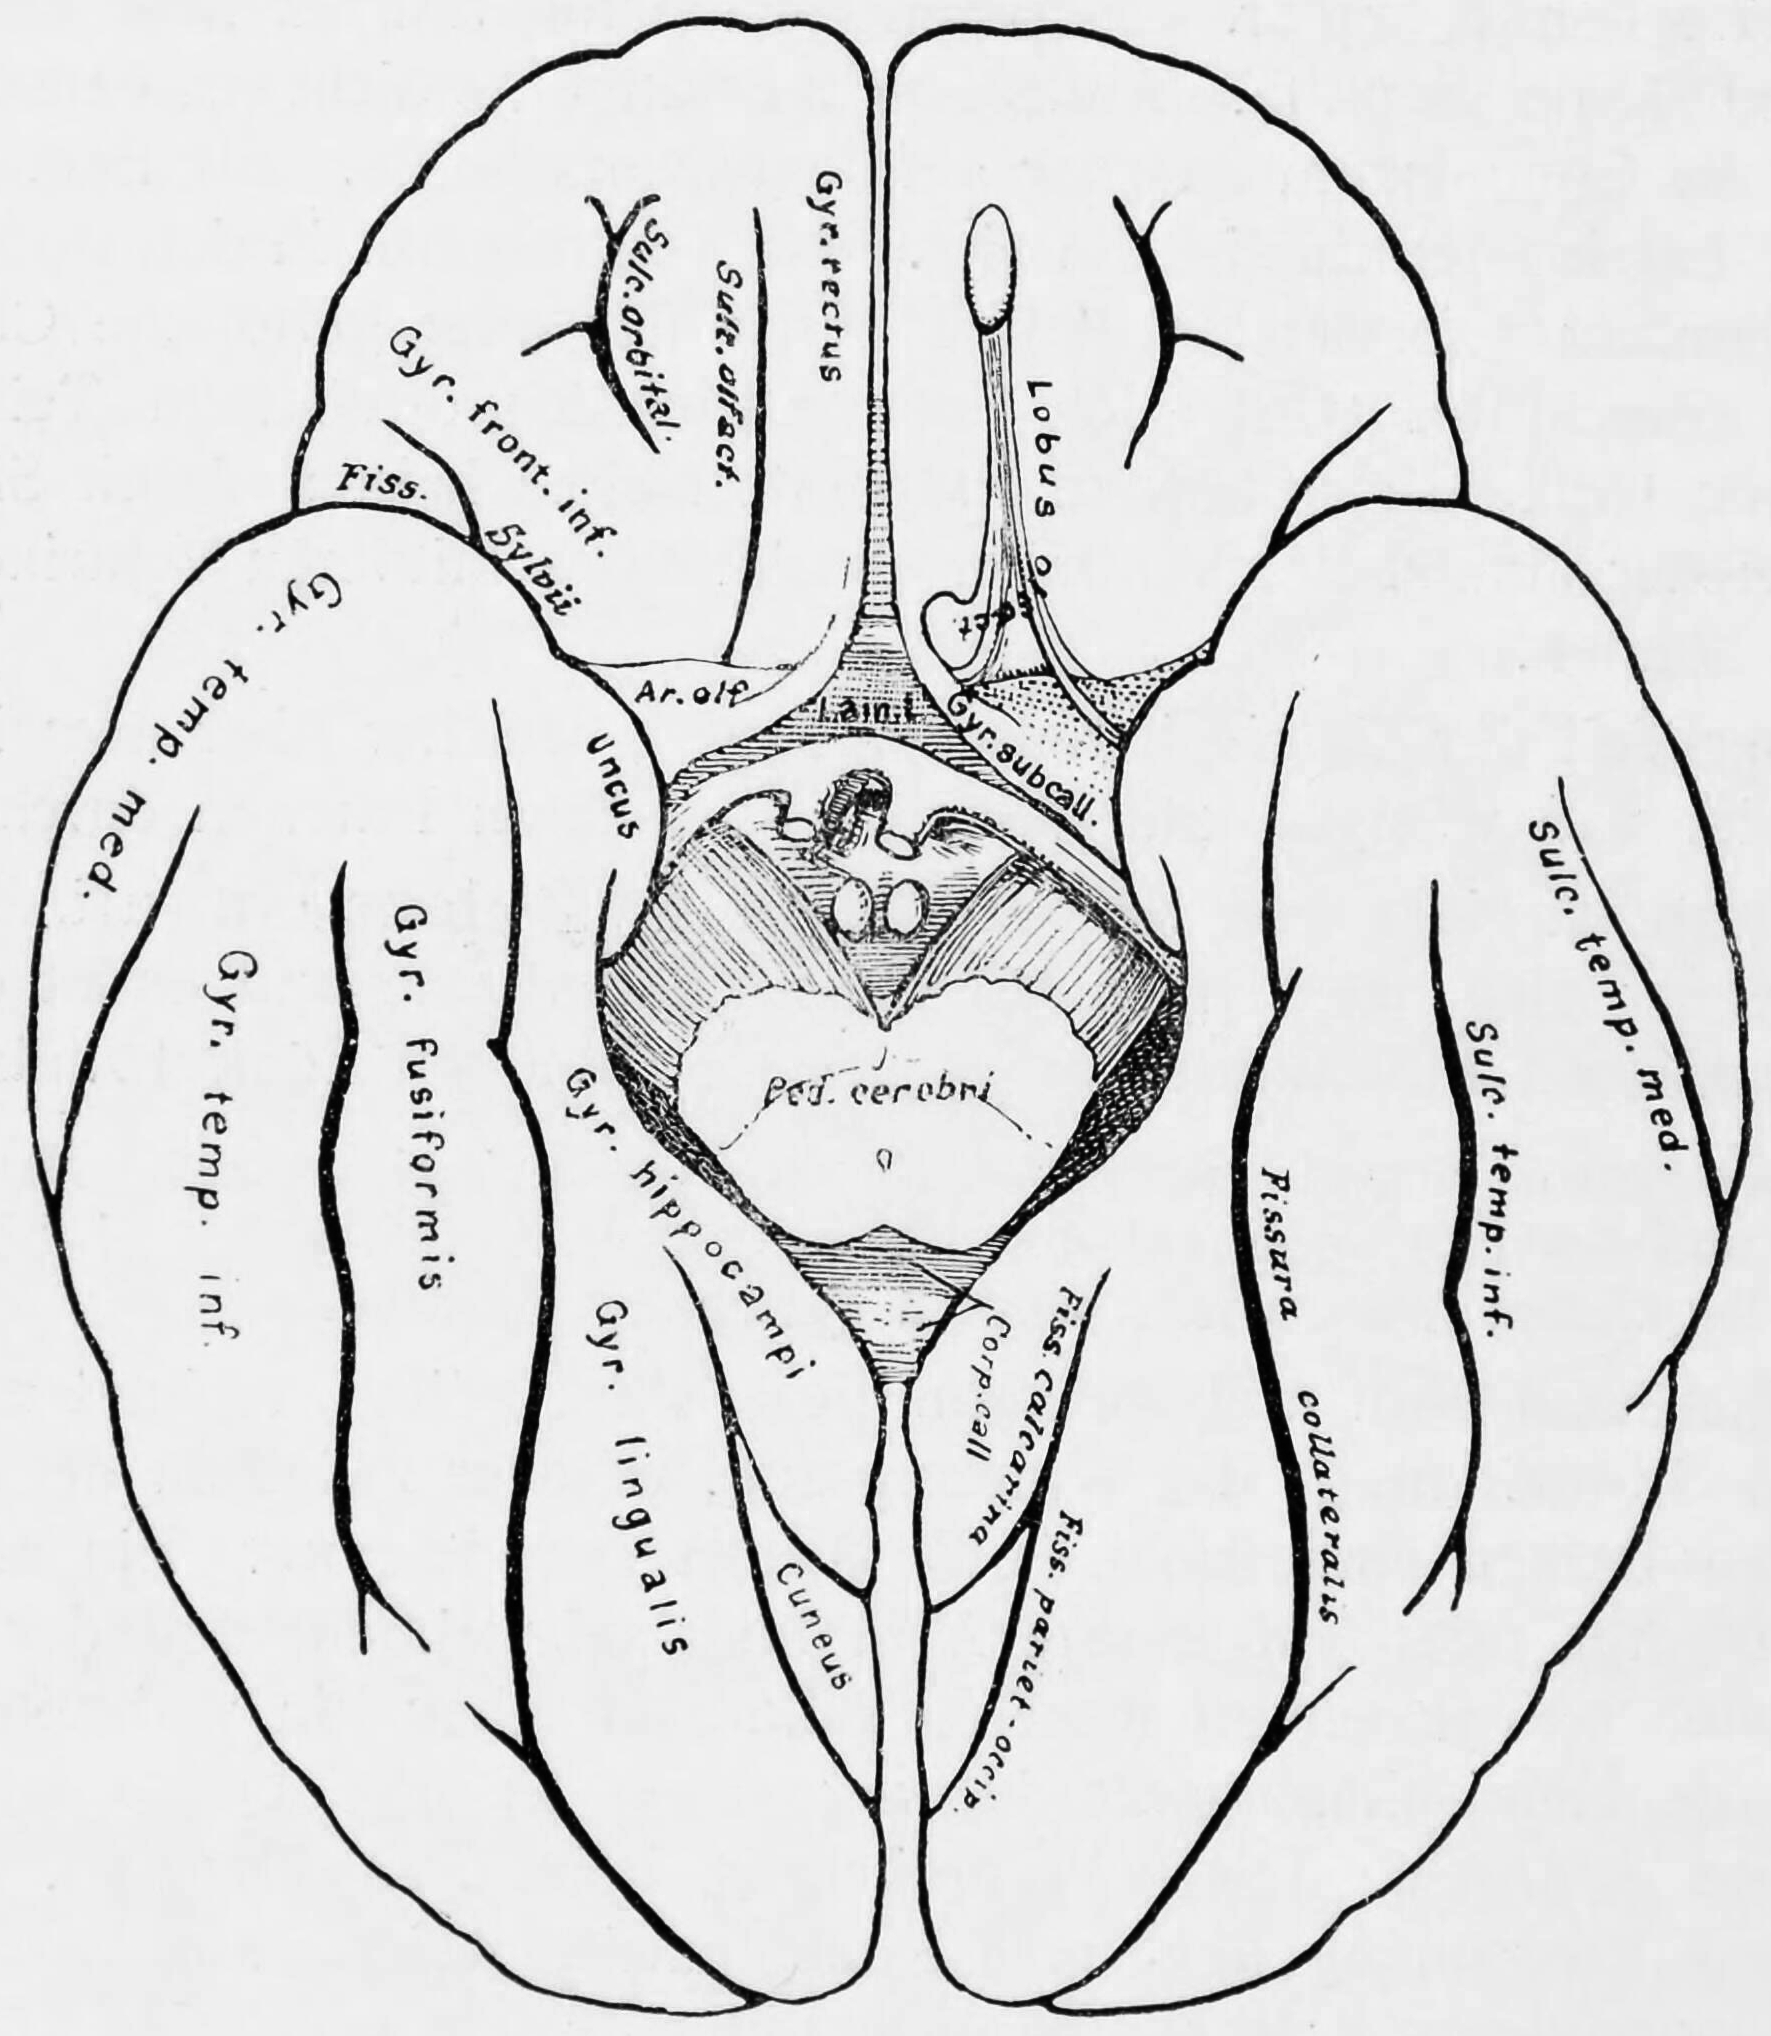
\includegraphics[width=0.7\linewidth]{./figures/nervoussystem/gyri_bot} 

}

\caption{Diagram showing a view from the bottom of the ridges (gyri) and grooves (sulci) of the left hemisphere of the brain.}\label{fig:gyribottom}
\end{figure}

Although the human brain represents only 2\% of the body weight, it receives 15\% of the cardiac output, 20\% of total body oxygen consumption, and 25\% of total body glucose utilization. The brain mostly uses glucose for energy, and deprivation of glucose, as can happen in hypoglycemia, can result in loss of consciousness. The energy consumption of the brain does not vary greatly over time, but active regions of the cortex consume somewhat more energy than inactive regions: this fact forms the basis for the functional brain imaging methods PET and fMRI. These functional imaging techniques provide a three-dimensional image of metabolic activity.

The simplest way to gain information about brain anatomy is by visual inspection, but many more sophisticated techniques have been developed. Brain tissue in its natural state is too soft to work with, but it can be hardened by immersion in alcohol or other fixatives, and then sliced apart for examination of the interior. Visually, the interior of the brain consists of areas of so-called grey matter, with a dark color, separated by areas of white matter, with a lighter color. Further information can be gained by staining slices of brain tissue with a variety of chemicals that bring out areas where specific types of molecules are present in high concentrations. It is also possible to examine the microstructure of brain tissue using a microscope, and to trace the pattern of connections from one brain area to another.

\hypertarget{development-of-the-nervous-system}{%
\section{Development Of The Nervous System}\label{development-of-the-nervous-system}}

All bilaterian animals at an early stage of development form a gastrula, which is polarized, with one end called the animal pole and the other the vegetal pole. The gastrula has the shape of a disk with three layers of cells, an inner layer called the endoderm, which gives rise to the lining of most internal organs, a middle layer called the mesoderm, which gives rise to the bones and muscles, and an outer layer called the ectoderm, which gives rise to the skin and nervous system.

In vertebrates, the first sign of the nervous system is the appearance of a thin strip of cells along the center of the back, called the neural plate. The inner portion of the neural plate (along the midline) is destined to become the central nervous system (CNS), the outer portion the peripheral nervous system (PNS). As development proceeds, a fold called the neural groove appears along the midline. This fold deepens, and then closes up at the top. At this point the future CNS appears as a cylindrical structure called the neural tube, whereas the future PNS appears as two strips of tissue called the neural crest, running lengthwise above the neural tube. The sequence of stages from neural plate to neural tube and neural crest is known as neurulation.

In the early 20\textsuperscript{th} century, a set of famous experiments by \href{https://en.wikipedia.org/wiki/Hans_Spemann}{Hans Spemann} and \href{https://en.wikipedia.org/wiki/Hilde_Mangold}{Hilde Mangold} showed that the formation of nervous tissue is ``induced'' by signals from a group of mesodermal cells called the organizer region. For decades, though, the nature of neural induction defeated every attempt to figure it out, until finally it was resolved by genetic approaches in the 1990s. Induction of neural tissue requires inhibition of the gene for a so-called bone morphogenetic protein, or BMP. Specifically the protein BMP4 appears to be involved. Two proteins called Noggin and Chordin, both secreted by the mesoderm, are capable of inhibiting BMP4 and thereby inducing ectoderm to turn into neural tissue. It appears that a similar molecular mechanism is involved for widely disparate types of animals, including arthropods as well as vertebrates. In some animals, however, another type of molecule called Fibroblast Growth Factor or FGF may also play an important role in induction.

Induction of neural tissues causes formation of neural precursor cells, called neuroblasts. In drosophila, neuroblasts divide asymmetrically, so that one product is a ``ganglion mother cell'' (GMC), and the other is a neuroblast. A GMC divides once, to give rise to either a pair of neurons or a pair of glial cells. In all, a neuroblast is capable of generating an indefinite number of neurons or glia.

One factor common to all bilateral organisms (including humans) is a family of secreted signaling molecules called neurotrophins which regulate the growth and survival of neurons. Because neurotrophins have now been identified in both vertebrate and invertebrates, this evidence suggests that neurotrophins were present in an ancestor common to bilateral organisms and may represent a common mechanism for nervous system formation.

\hypertarget{the-function-of-the-nervous-system}{%
\section{The Function Of The Nervous System}\label{the-function-of-the-nervous-system}}

Organisms need information to solve at least three kinds of problems: (a) to maintain an appropriate environment, i.e., homeostasis; (b) to time activities (e.g., seasonal changes in behavior) or synchronize activities with those of conspecifics; and (c) to locate and respond to resources or threats (e.g., by moving towards resources or evading or attacking threats). Organisms also need to transmit information in order to influence another's behavior: to identify themselves, warn conspecifics of danger, coordinate activities, or deceive.

At the most basic level, the function of the nervous system is to send signals from one cell to others, or from one part of the body to others. There are multiple ways that a cell can send signals to other cells. One is by releasing chemicals called hormones into the internal circulation, so that they can diffuse to distant sites. In contrast to this ``broadcast'' mode of signaling, the nervous system provides ``point-to-point'' signals---neurons project their axons to specific target areas and make synaptic connections with specific target cells. Thus, neural signaling is capable of a much higher level of specificity than hormonal signaling. It is also much faster: the fastest nerve signals travel at speeds that exceed 100 meters per second.

At a more integrative level, the primary function of the nervous system is to control the body. It does this by extracting information from the environment using sensory receptors, sending signals that encode this information into the central nervous system, processing the information to determine an appropriate response, and sending output signals to muscles or glands to activate the response. The evolution of a complex nervous system has made it possible for various animal species to have advanced perception abilities such as vision, complex social interactions, rapid coordination of organ systems, and integrated processing of concurrent signals. In humans, the sophistication of the nervous system makes it possible to have language, abstract representation of concepts, transmission of culture, and many other features of human society that would not exist without the human brain.

\hypertarget{the-sensory-system}{%
\section{The Sensory System}\label{the-sensory-system}}

The sensory nervous system is a part of the nervous system responsible for processing sensory information. A sensory system consists of sensory neurons (including the sensory receptor cells), neural pathways, and parts of the brain involved in sensory perception. Commonly recognized sensory systems are those for vision, hearing, touch, taste, smell, and balance. In short, senses are transducers from the physical world to the realm of the mind where we interpret the information, creating our perception of the world around us.

Sensory systems code for four aspects of a stimulus; type (modality), intensity, location, and duration. Arrival time of a sound pulse and phase differences of continuous sound are used for sound localization. Certain receptors are sensitive to certain types of stimuli (for example, different mechanoreceptors respond best to different kinds of touch stimuli, like sharp or blunt objects). Receptors send impulses in certain patterns to send information about the intensity of a stimulus (for example, how loud a sound is). The location of the receptor that is stimulated gives the brain information about the location of the stimulus (for example, stimulating a mechanoreceptor in a finger will send information to the brain about that finger). The duration of the stimulus (how long it lasts) is conveyed by firing patterns of receptors. These impulses are transmitted to the brain through afferent neurons.

While debate exists among neurologists as to the specific number of senses due to differing definitions of what constitutes a sense, Gautama Buddha and Aristotle classified five `traditional' human senses which have become universally accepted: touch, taste, smell, sight, and hearing. Other senses that have been well-accepted in most mammals, including humans, include nociception, equilibrioception, kinaesthesia, and thermoception. Furthermore, some nonhuman animals have been shown to possess alternate senses, including magnetoception and electroreception.

The human sensory system consists of the following subsystems:

\begin{itemize}
\tightlist
\item
  Somatosensory system consists of the receptors, transmitters (pathways) leading to area S1, and area S1 in the cortex that is involved in creating the conscious experience of the sensations labelled as touch or pressure, temperature (warm or cold), pain (including itch and tickle), and the sensations of muscle movement and joint position including posture, movement, and facial expression (collectively also called proprioception)
\item
  Visual system
\item
  Auditory system
\item
  Vestibular system
\item
  Olfactory system
\item
  Gustatory system
\end{itemize}

The receptive field is the area of the body or environment to which a receptor organ and receptor cells respond. For instance, the part of the world an eye can see, is its receptive field; the light that each rod or cone can see, is its receptive field. Receptive fields have been identified for the visual system, auditory system and somatosensory system.

\hypertarget{the-motor-system}{%
\section{The Motor System}\label{the-motor-system}}

The motor system is the set of central and peripheral structures in the nervous system that support motor functions, i.e.~movement. Peripheral structures may include skeletal muscles and neural connections with muscle tissues. Central structures include cerebral cortex, brainstem, spinal cord, pyramidal system including the upper motor neurons, extrapyramidal system, cerebellum, and the lower motor neurons in the brainstem and the spinal cord.

The pyramidal motor system, also called the pyramidal tract or the corticospinal tract, start in the motor center of the cerebral cortex. There are upper and lower motor neurons in the corticospinal tract. The motor impulses originate in the giant pyramidal cells or Betz cells of the motor area; i.e., precentral gyrus of cerebral cortex. These are the upper motor neurons (UMN) of the corticospinal tract. The axons of these cells pass in the depth of the cerebral cortex to the corona radiata and then to the internal capsule passing through the posterior branch of internal capsule and continue to descend in the midbrain and the medulla oblongata. In the lower part of medulla oblongata 80 to 85\% of these fibers decussate (pass to the opposite side) and descend in the white matter of the lateral funiculus of the spinal cord on the opposite side. The remaining 15 to 20\% pass to the same side. Fibers for the extremities (limbs) pass 100\% to the opposite side. The fibers of the corticospinal tract terminate at different levels in the anterior horn of the grey matter of the spinal cord. Here the lower motor neurons (LMN) of the spinal cord are located. Peripheral motor nerves carry the motor impulses from the anterior horn to the voluntary muscles.

The extrapyramidal system is called extrapyramidal to distinguish it from the tracts of the motor cortex that reach their targets by traveling through the pyramids of the medulla. The pyramidal tracts (corticospinal tract and corticobulbar tracts) may directly innervate motor neurons of the spinal cord or brainstem (anterior (ventral) horn cells or certain cranial nerve nuclei), whereas the extrapyramidal system centers on the modulation and regulation (indirect control) of anterior (ventral) horn cells.

Extrapyramidal tracts are chiefly found in the reticular formation of the pons and medulla, and target lower motor neurons in the spinal cord that are involved in reflexes, locomotion, complex movements, and postural control. These tracts are in turn modulated by various parts of the central nervous system, including the nigrostriatal pathway, the basal ganglia, the cerebellum, the vestibular nuclei, and different sensory areas of the cerebral cortex. All of these regulatory components can be considered part of the extrapyramidal system, in that they modulate motor activity without directly innervating motor neurons.

\hypertarget{neuronal-signalling}{%
\section{Neuronal Signalling}\label{neuronal-signalling}}

Most neurons send signals via their axons, although some types are capable of dendrite-to-dendrite communication. (In fact, the types of neurons in the retina of the eye called amacrine cells have no axons, and communicate only via their dendrites.) Neural signals propagate along an axon in the form of electrochemical waves called action potentials, which produce cell-to-cell signals at points where axon terminals make synaptic contact with other cells.

Synapses may be electrical or chemical. Electrical synapses make direct electrical connections between neurons, but chemical synapses are much more common, and much more diverse in function. At a chemical synapse, the cell that sends signals is called presynaptic, and the cell that receives signals is called postsynaptic. Both the presynaptic and postsynaptic areas are full of molecular machinery that carries out the signalling process. The presynaptic area contains large numbers of tiny spherical vessels called synaptic vesicles, packed with neurotransmitter chemicals. When the presynaptic terminal is electrically stimulated, an array of molecules embedded in the membrane are activated, and cause the contents of the vesicles to be released into the narrow space between the presynaptic and postsynaptic membranes, called the synaptic cleft. The neurotransmitter then binds to receptors embedded in the postsynaptic membrane, causing them to enter an activated state. Depending on the type of receptor, the resulting effect on the postsynaptic cell may be excitatory, inhibitory, or modulatory in more complex ways. For example, release of the neurotransmitter acetylcholine at a synaptic contact between a motor neuron and a muscle cell induces rapid contraction of the muscle cell. The entire synaptic transmission process takes only a fraction of a millisecond, although the effects on the postsynaptic cell may last much longer (even indefinitely, in cases where the synaptic signal leads to the formation of a memory trace).

There are literally hundreds of different types of synapses. In fact, there are over a hundred known neurotransmitters, and many of them have multiple types of receptors. Many synapses use more than one neurotransmitter---a common arrangement is for a synapse to use one fast-acting small-molecule neurotransmitter such as glutamate or GABA, along with one or more peptide neurotransmitters that play slower-acting modulatory roles. Molecular neuroscientists generally divide receptors into two broad groups: chemically gated ion channels and second messenger systems. When a chemically gated ion channel is activated, it forms a passage that allows specific types of ions to flow across the membrane. Depending on the type of ion, the effect on the target cell may be excitatory or inhibitory. When a second messenger system is activated, it starts a cascade of molecular interactions inside the target cell, which may ultimately produce a wide variety of complex effects, such as increasing or decreasing the sensitivity of the cell to stimuli, or even altering gene transcription.

According to a rule called Dale's principle, which has only a few known exceptions, a neuron releases the same neurotransmitters at all of its synapses. This does not mean, though, that a neuron exerts the same effect on all of its targets, because the effect of a synapse depends not on the neurotransmitter, but on the receptors that it activates. Because different targets can (and frequently do) use different types of receptors, it is possible for a neuron to have excitatory effects on one set of target cells, inhibitory effects on others, and complex modulatory effects on others still. Nevertheless, it happens that the two most widely used neurotransmitters, glutamate and GABA, each have largely consistent effects. Glutamate has several widely occurring types of receptors, but all of them are excitatory or modulatory. Similarly, GABA has several widely occurring receptor types, but all of them are inhibitory. Because of this consistency, glutamatergic cells are frequently referred to as ``excitatory neurons'', and GABAergic cells as ``inhibitory neurons''. Strictly speaking, this is an abuse of terminology---it is the receptors that are excitatory and inhibitory, not the neurons---but it is commonly seen even in scholarly publications.

One very important subset of synapses are capable of forming memory traces by means of long-lasting activity-dependent changes in synaptic strength. The best-known form of neural memory is a process called long-term potentiation (abbreviated LTP), which operates at synapses that use the neurotransmitter glutamate acting on a special type of receptor known as the NMDA receptor. The NMDA receptor functions as a molecular ``conincidence detector'': although the NMDA-receptor associated ion-channel opens upon binding of glutamate, extracellular Mg\textsuperscript{2+} ions will enter and block the channel immediately. Only concomitant membrane depolarization (e.g.~induced by Na\textsuperscript{+} influx via concomittantly stimulated non-NMDA (AMPA) type glutamate receptors in the same cell), will overcome the Mg\textsuperscript{2+} block and allow Na\textsuperscript{+} and Ca\textsuperscript{2+} ions to enter the cell thourgh the NMDA-receptor. Calcium entering the postsynaptic cell via NMDA receptors then initiates a second messenger cascade that ultimately leads to an increase in the number of AMPA-type glutamate receptors in the target cell, thereby increasing the effective strength of the synapse. This change in strength can last for weeks or longer. Besides the NMDA-receptor based processes, further cellular mechanisms allow of the association between two different input signals converging on the same neuron, in a defined timeframe. Upon a simultaneous increase in the intracellular concentrations of cAMP and Ca2+, a transcriptional coactivator called TORC1 (CRTC1) becomes activated, that converts the temporal coincidence of the two second messengers into long term changes such as LTP. This cellular mechanism, through calcium-dependent adenylate cyclase activation, might also account for the detection of the repetitive stimulation of a given synapse.

In 1949, \href{https://en.wikipedia.org/wiki/Donald_O._Hebb}{Donald Hebb} postulated that synaptic efficiency will increase through repeated and persistent stimulation of a postsynaptic cell by a presynaptic cell. This is often informally summarized as ``cells that fire together, wire together''. The theory was validated in part by the discovery of long-term potentiation. Studies of LTP on multiple presynaptic cells stimulating a postsynaptic cell uncovered the property of associativity. A weak neuronal stimulation onto a pyramidal neuron may not induce long-term potentiation. However, this same stimulation paired with a simultaneous strong stimulation from another neuron will strengthen both synapses. This process suggests that two neuronal pathways converging on the same cell may both strengthen if stimulated coincidentally.

Since the discovery of LTP in 1973, many other types of synaptic memory traces have been found, involving increases or decreases in synaptic strength that are induced by varying conditions, and last for variable periods of time. The reward system, that reinforces desired behaviour for example, depends on a variant form of LTP that is conditioned on an extra input coming from a reward-signalling pathway that uses dopamine as neurotransmitter. All these forms of synaptic modifiability, taken collectively, give rise to neural plasticity, that is, to a capability for the nervous system to adapt itself to variations in the environment.

\hypertarget{neurons-and-glial-cells}{%
\section{Neurons And Glial Cells}\label{neurons-and-glial-cells}}

\hypertarget{neurons}{%
\subsection{Neurons}\label{neurons}}

The neuron doctrine is the now fundamental idea that neurons are the basic structural and functional units of the nervous system. The theory was put forward by Santiago Ramón y Cajal in the late 19th century. It held that neurons are discrete cells (not connected in a meshwork), acting as metabolically distinct units.

Later discoveries yielded refinements to the doctrine. For example, glial cells, which are not considered neurons, play an essential role in information processing. Also, electrical synapses are more common than previously thought, comprising direct, cytoplasmic connections between neurons. In fact, neurons can form even tighter couplings: the squid giant axon arises from the fusion of multiple axons.

Ramón y Cajal also postulated the Law of Dynamic Polarization, which states that a neuron receives signals at its dendrites and cell body and transmits them, as action potentials, along the axon in one direction: away from the cell body. The Law of Dynamic Polarization has important exceptions; dendrites can serve as synaptic output sites of neurons and axons can receive synaptic inputs.

The number of neurons in the brain varies dramatically from species to species. In a human, there are an estimated 10--20 billion neurons in the cerebral cortex and 55--70 billion neurons in the cerebellum. By contrast, the nematode worm \emph{Caenorhabditis elegans} has just 302 neurons, making it an ideal model organism as scientists have been able to map all of its neurons. The fruit fly \emph{Drosophila melanogaster}, a common subject in biological experiments, has around 100,000 neurons and exhibits many complex behaviors. Many properties of neurons, from the type of neurotransmitters used to ion channel composition, are maintained across species, allowing scientists to study processes occurring in more complex organisms in much simpler experimental systems.

A neuron, neurone (old British spelling) or nerve cell, is an electrically excitable cell that communicates with other cells via specialized connections called synapses. It is the main component of nervous tissue. All animals except sponges and placozoans have neurons, but other multicellular organisms such as plants do not.

Neurons are typically classified into three types based on their function. Sensory neurons respond to stimuli such as touch, sound, or light that affect the cells of the sensory organs, and they send signals to the spinal cord or brain. Motor neurons receive signals from the brain and spinal cord to control everything from muscle contractions to glandular output. Interneurons connect neurons to other neurons within the same region of the brain or spinal cord. A group of connected neurons is called a neural circuit.

A typical neuron consists of a cell body (soma), dendrites, and a single axon. The soma is usually compact. The axon and dendrites are filaments that extrude from it. Dendrites typically branch profusely and extend a few hundred micrometers from the soma. The axon leaves the soma at a swelling called the axon hillock, and travels for as far as 1 meter in humans or more in other species. It branches but usually maintains a constant diameter. At the farthest tip of the axon's branches are axon terminals, where the neuron can transmit a signal across the synapse to another cell. Neurons may lack dendrites or have no axon. The term neurite is used to describe either a dendrite or an axon, particularly when the cell is undifferentiated.

Most neurons receive signals via the dendrites and soma and send out signals down the axon. At the majority of synapses, signals cross from the axon of one neuron to a dendrite of another. However, synapses can connect an axon to another axon or a dendrite to another dendrite.

The signaling process is partly electrical and partly chemical. Neurons are electrically excitable, due to maintenance of voltage gradients across their membranes. If the voltage changes by a large enough amount over a short interval, the neuron generates an all-or-nothing electrochemical pulse called an action potential. This potential travels rapidly along the axon, and activates synaptic connections as it reaches them. Synaptic signals may be excitatory or inhibitory, increasing or reducing the net voltage that reaches the soma.

In most cases, neurons are generated by neural stem cells during brain development and childhood. Neurogenesis largely ceases during adulthood in most areas of the brain. However, strong evidence supports generation of substantial numbers of new neurons in the hippocampus and olfactory bulb.

Neurons are highly specialized for the processing and transmission of cellular signals. Given their diversity of functions performed in different parts of the nervous system, there is a wide variety in their shape, size, and electrochemical properties. For instance, the soma of a neuron can vary from 4 to 100 micrometers in diameter.

The soma is the body of the neuron. As it contains the nucleus, most protein synthesis occurs here. The nucleus can range from 3 to 18 micrometers in diameter.
The dendrites of a neuron are cellular extensions with many branches. This overall shape and structure is referred to metaphorically as a dendritic tree. This is where the majority of input to the neuron occurs via the dendritic spine.

The axon is a finer, cable-like projection that can extend tens, hundreds, or even tens of thousands of times the diameter of the soma in length. The axon primarily carries nerve signals away from the soma, and carries some types of information back to it. Many neurons have only one axon, but this axon may---and usually will---undergo extensive branching, enabling communication with many target cells. The part of the axon where it emerges from the soma is called the axon hillock. Besides being an anatomical structure, the axon hillock also has the greatest density of voltage-dependent sodium channels. This makes it the most easily excited part of the neuron and the spike initiation zone for the axon. In electrophysiological terms, it has the most negative threshold potential. While the axon and axon hillock are generally involved in information outflow, this region can also receive input from other neurons.

The axon terminal is found at the end of the axon farthest from the soma and contains synapses. Synaptic boutons are specialized structures where neurotransmitter chemicals are released to communicate with target neurons. In addition to synaptic boutons at the axon terminal, a neuron may have en passant boutons, which are located along the length of the axon.

The accepted view of the neuron attributes dedicated functions to its various anatomical components; however, dendrites and axons often act in ways contrary to their so-called main function.

Axons and dendrites in the central nervous system are typically only about one micrometer thick, while some in the peripheral nervous system are much thicker. The soma is usually about 10--25 micrometers in diameter and often is not much larger than the cell nucleus it contains. The longest axon of a human motor neuron can be over a meter long, reaching from the base of the spine to the toes.

Sensory neurons can have axons that run from the toes to the posterior column of the spinal cord, over 1.5 meters in adults. Giraffes have single axons several meters in length running along the entire length of their necks. Much of what is known about axonal function comes from studying the squid giant axon, an ideal experimental preparation because of its relatively immense size (0.5--1 millimeters thick, several centimeters long).

Fully differentiated neurons are permanently postmitotic however, stem cells present in the adult brain may regenerate functional neurons throughout the life of an organism. Astrocytes are star-shaped glial cells. They have been observed to turn into neurons by virtue of their stem cell-like characteristic of pluripotency.

Like all animal cells, the cell body of every neuron is enclosed by a plasma membrane, a bilayer of lipid molecules with many types of protein structures embedded in it. A lipid bilayer is a powerful electrical insulator, but in neurons, many of the protein structures embedded in the membrane are electrically active. These include ion channels that permit electrically charged ions to flow across the membrane and ion pumps that transport ions from one side of the membrane to the other. Most ion channels are permeable only to specific types of ions. Some ion channels are voltage gated, meaning that they can be switched between open and closed states by altering the voltage difference across the membrane. Others are chemically gated, meaning that they can be switched between open and closed states by interactions with chemicals that diffuse through the extracellular fluid. The ions include sodium, potassium, chloride, and calcium. The interactions between ion channels and ion pumps produce a voltage difference across the membrane, typically a bit less than 1/10 of a volt at baseline. This voltage has two functions: first, it provides a power source for an assortment of voltage-dependent protein machinery that is embedded in the membrane; second, it provides a basis for electrical signal transmission between different parts of the membrane.

Numerous microscopic clumps called Nissl bodies (or Nissl substance) are seen when nerve cell bodies are stained with a basophilic (``base-loving'') dye. These structures consist of rough endoplasmic reticulum and associated ribosomal RNA. Named after German psychiatrist and neuropathologist \href{https://en.wikipedia.org/wiki/Franz_Nissl}{Franz Nissl} (1860--1919), they are involved in protein synthesis and their prominence can be explained by the fact that nerve cells are very metabolically active. Basophilic dyes such as aniline or (weakly) haematoxylin highlight negatively charged components, and so bind to the phosphate backbone of the ribosomal RNA.

The cell body of a neuron is supported by a complex mesh of structural proteins called neurofilaments, which together with neurotubules (neuronal microtubules) are assembled into larger neurofibrils. Some neurons also contain pigment granules, such as neuromelanin (a brownish-black pigment that is byproduct of synthesis of catecholamines), and lipofuscin (a yellowish-brown pigment), both of which accumulate with age. Other structural proteins that are important for neuronal function are actin and the tubulin of microtubules. Class III β-tubulin is found almost exclusively in neurons. Actin is predominately found at the tips of axons and dendrites during neuronal development. There the actin dynamics can be modulated via an interplay with microtubule.



\begin{figure}

{\centering 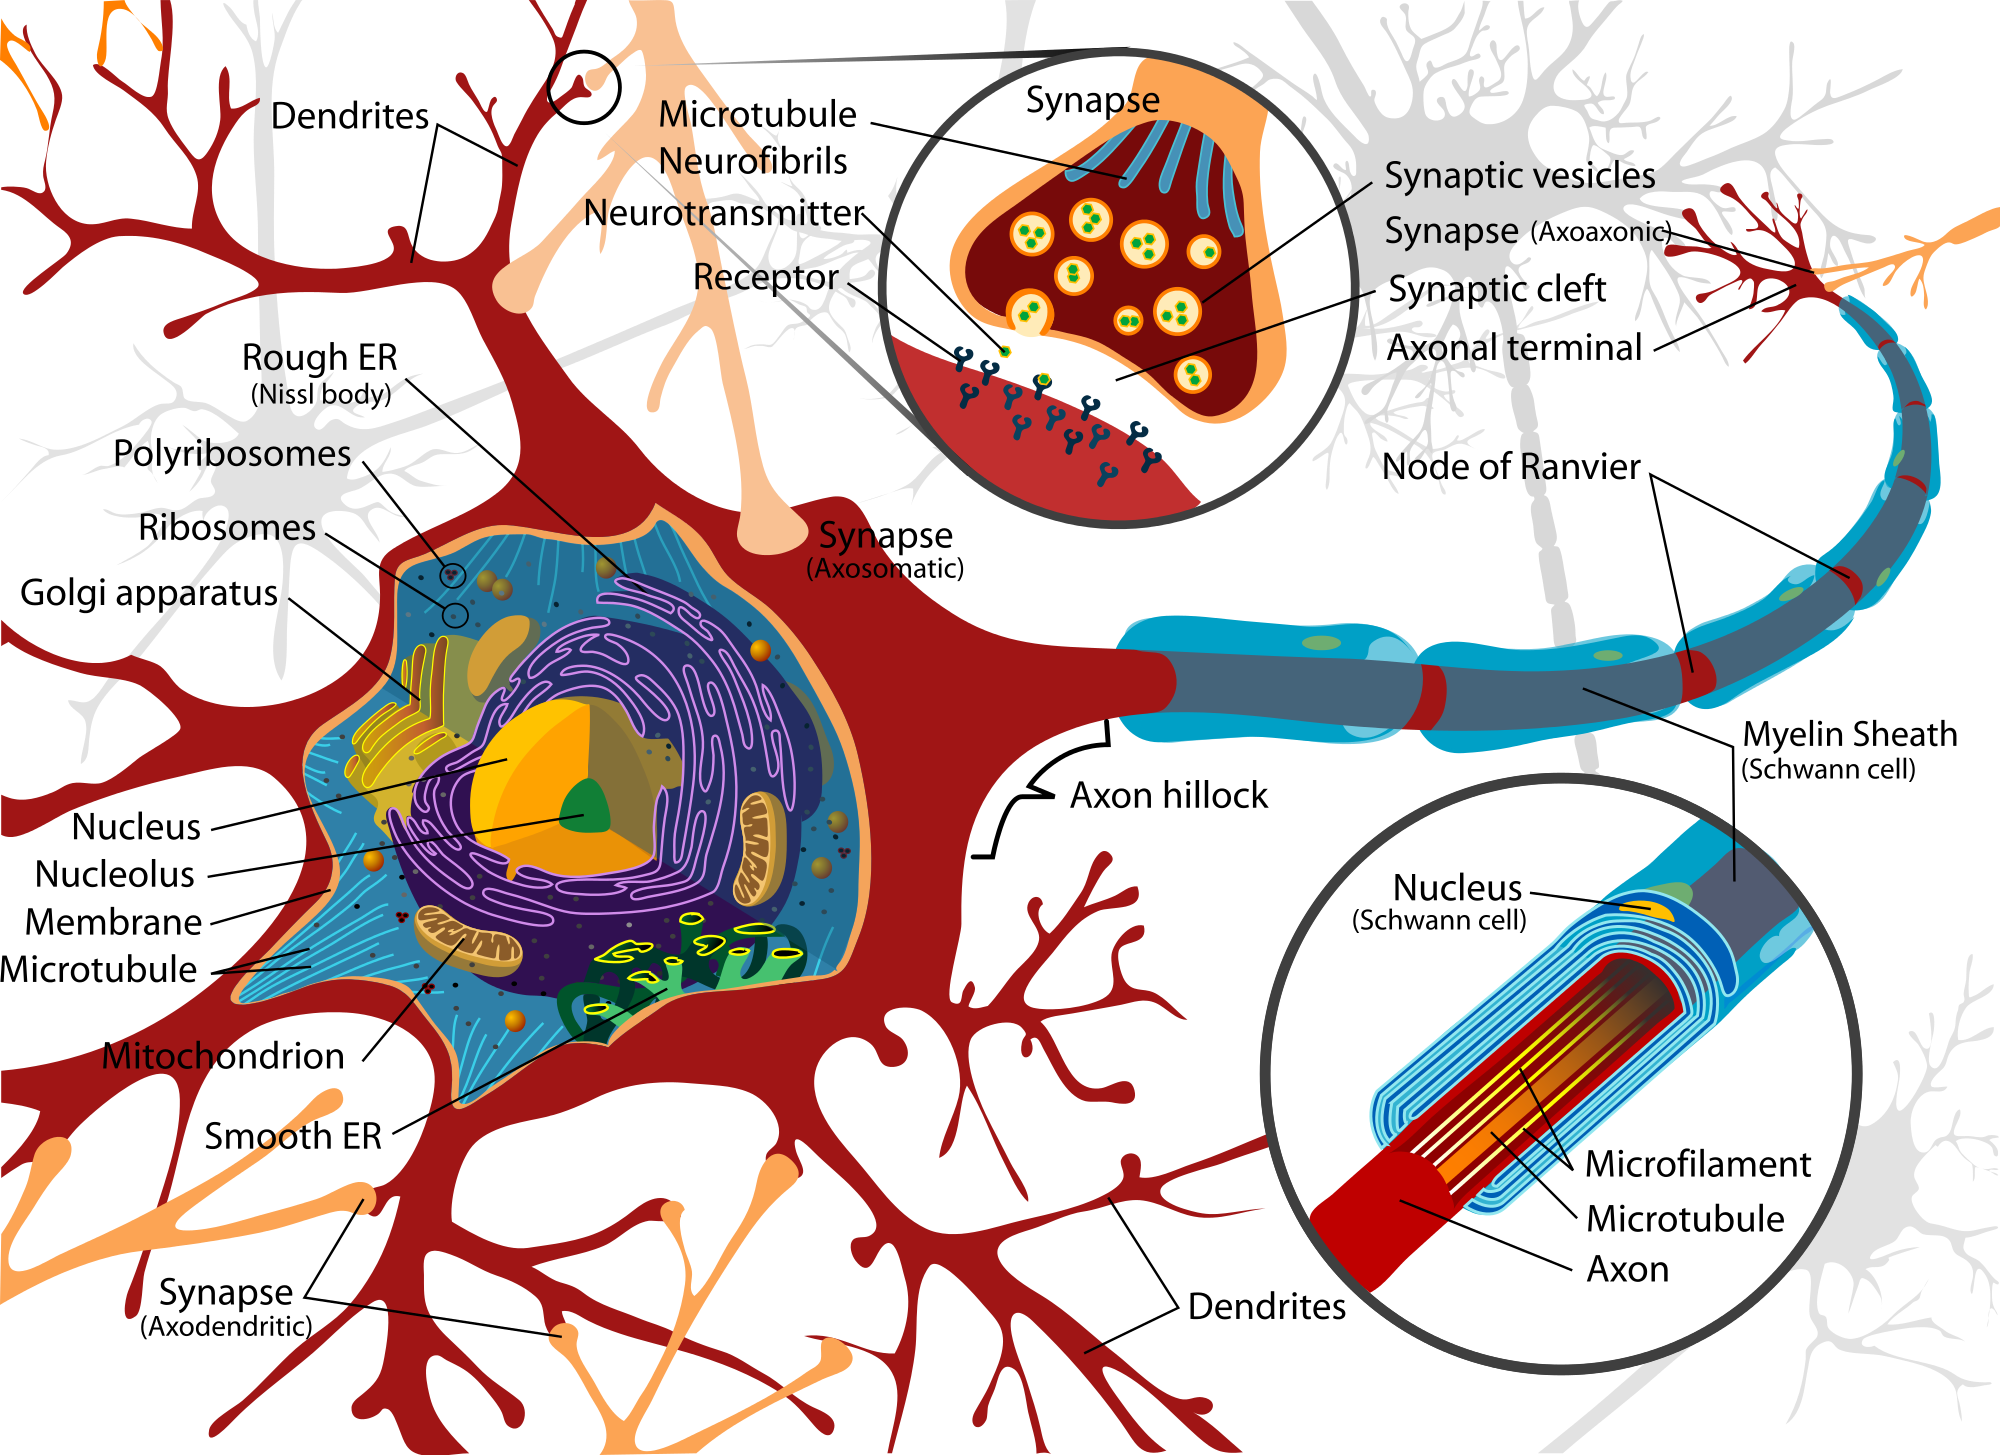
\includegraphics[width=0.7\linewidth]{./figures/cells/Complete_neuron_cell_diagram_en} 

}

\caption{\href{https://commons.wikimedia.org/wiki/File:Complete_neuron_cell_diagram_en.svg}{Diagram of a myelinated vertebrate motor neuron.}}\label{fig:motorneuron}
\end{figure}

There are different internal structural characteristics between axons and dendrites. Typical axons almost never contain ribosomes, except some in the initial segment. Dendrites contain granular endoplasmic reticulum or ribosomes, in diminishing amounts as the distance from the cell body increases.

Neurons vary in shape and size and can be classified by their morphology and function. The anatomist \href{https://en.wikipedia.org/wiki/Camillo_Golgi}{Camillo Golgi} grouped neurons into two types; type I with long axons used to move signals over long distances and type II with short axons, which can often be confused with dendrites. Type I cells can be further classified by the location of the soma. The basic morphology of type I neurons, represented by spinal motor neurons, consists of a cell body called the soma and a long thin axon covered by a myelin sheath.

The dendritic tree wraps around the cell body and receives signals from other neurons. The end of the axon has branching terminals (axon terminal) that release neurotransmitters into a gap called the synaptic cleft between the terminals and the dendrites of the next neuron.

Most neurons can be anatomically characterized as:

\begin{itemize}
\tightlist
\item
  Unipolar: single process
\item
  Bipolar: 1 axon and 1 dendrite
\item
  Multipolar: 1 axon and 2 or more dendrites
\item
  Golgi I: neurons with projecting axonal processes; examples are pyramidal cells, Purkinje cells, and anterior horn cells
\item
  Golgi II: neurons whose axonal process projects locally; the best example is the granule cell
\item
  Anaxonic: where the axon cannot be distinguished from the dendrite(s)
\item
  Pseudounipolar: 1 process which then serves as both an axon and a dendrite
\item
  Other
\end{itemize}



\begin{figure}

{\centering \includegraphics[width=0.7\linewidth]{./figures/cells/Cajal_neurons} 

}

\caption{Morpholoigcally distinct types of neurons after Cajal. A) Unipolar neurons; B) bipolar neurons; Golgi I neurons: C) a Purkinje cell; D) spinal motor neuron E) a pyramidal cell; F) Golgi II neuron. \href{https://wellcomelibrary.org/item/b2129592x\#?c=0\&m=0\&s=0\&cv=14\&z=0\%2C-3.48\%2C1\%2C8.6591}{Histologie du système nerveux de l'homme \& des vertébrés, Tome Premier} (1909) by Santiago Ramón y Cajal translated from Spanish by Dr.~L. Azoulay.}\label{fig:neurontypes}
\end{figure}

Neurons can also be characterized based on various aspects of their function:

\begin{itemize}
\tightlist
\item
  Afferent neurons convey information from tissues and organs into the central nervous system and are also called sensory neurons.
\item
  Efferent neurons (motor neurons) transmit signals from the central nervous system to the effector cells.
\item
  Interneurons connect neurons within specific regions of the central nervous system.
  Afferent and efferent also refer generally to neurons that, respectively, bring information to or send information from the brain.
\end{itemize}

The axons of neurons in the human peripheral nervous system can be classified based on their physical features and signal conduction properties. Axons were known to have different thicknesses (from 0.1 to 20 µm) and these differences were thought to relate to the speed at which an action potential could travel along the axon -- its conductance velocity. Erlanger and Gasser proved this hypothesis, and identified several types of nerve fiber, establishing a relationship between the diameter of an axon and its nerve conduction velocity. They published their findings in 1941 giving the first classification of axons.

Neurons communicate with each another via synapses, where either the axon terminal of one cell contacts another neuron's dendrite, soma or, less commonly, axon. Neurons such as Purkinje cells in the cerebellum can have over 1000 dendritic branches, making connections with tens of thousands of other cells; other neurons, such as the magnocellular neurons of the supraoptic nucleus, have only one or two dendrites, each of which receives thousands of synapses.

Synapses can be excitatory or inhibitory, either increasing or decreasing activity in the target neuron, respectively. Some neurons also communicate via electrical synapses, which are direct, electrically conductive junctions between cells.

When an action potential reaches the axon terminal, it opens voltage-gated calcium channels, allowing calcium ions to enter the terminal. Calcium causes synaptic vesicles filled with neurotransmitter molecules to fuse with the membrane, releasing their contents into the synaptic cleft. The neurotransmitters diffuse across the synaptic cleft and activate receptors on the postsynaptic neuron. High cytosolic calcium in the axon terminal triggers mitochondrial calcium uptake, which, in turn, activates mitochondrial energy metabolism to produce ATP to support continuous neurotransmission.

An autapse is a synapse in which a neuron's axon connects to its own dendrites.

The human brain has some 8.6 x 10\textsuperscript{10} (eighty six billion) neurons. Each neuron has on average 7,000 synaptic connections to other neurons. It has been estimated that the brain of a three-year-old child has about 10\textsuperscript{15} synapses (1 quadrillion). This number declines with age, stabilizing by adulthood. Estimates vary for an adult, ranging from 10\textsuperscript{14} to 5 x 10\textsuperscript{14} synapses (100 to 500 trillion).

The two most common neurotransmitters in the brain, glutamate and GABA, have largely consistent actions. Glutamate acts on several types of receptors, and has effects that are excitatory at ionotropic receptors and a modulatory effect at metabotropic receptors. Similarly, GABA acts on several types of receptors, but all of them have inhibitory effects (in adult animals, at least). Because of this consistency, it is common for neuroscientists to refer to cells that release glutamate as ``excitatory neurons'', and cells that release GABA as ``inhibitory neurons''. Some other types of neurons have consistent effects, for example, ``excitatory'' motor neurons in the spinal cord that release acetylcholine, and ``inhibitory'' spinal neurons that release glycine.

The distinction between excitatory and inhibitory neurotransmitters is not absolute. Rather, it depends on the class of chemical receptors present on the postsynaptic neuron. In principle, a single neuron, releasing a single neurotransmitter, can have excitatory effects on some targets, inhibitory effects on others, and modulatory effects on others still. For example, photoreceptor cells in the retina constantly release the neurotransmitter glutamate in the absence of light. So-called OFF bipolar cells are, like most neurons, excited by the released glutamate. However, neighboring target neurons called ON bipolar cells are instead inhibited by glutamate, because they lack typical ionotropic glutamate receptors and instead express a class of inhibitory metabotropic glutamate receptors. When light is present, the photoreceptors cease releasing glutamate, which relieves the ON bipolar cells from inhibition, activating them; this simultaneously removes the excitation from the OFF bipolar cells, silencing them.

Neurons can also be classified based on the neurotransmitter they release at synapses:

\begin{itemize}
\tightlist
\item
  Cholinergic neurons---acetylcholine. Acetylcholine is released from presynaptic neurons into the synaptic cleft. It acts as a ligand for both ligand-gated ion channels and metabotropic (GPCRs) muscarinic receptors. Nicotinic receptors are pentameric ligand-gated ion channels composed of alpha and beta subunits that bind nicotine. Ligand binding opens the channel causing influx of Na\textsuperscript{+} depolarization and increases the probability of presynaptic neurotransmitter release. Acetylcholine is synthesized from choline and acetyl coenzyme A.
\item
  GABAergic neurons---gamma aminobutyric acid. GABA is one of two neuroinhibitors in the central nervous system (CNS), along with glycine. GABA has a homologous function to ACh, gating anion channels that allow Cl\textsuperscript{−} ions to enter the post synaptic neuron. Cl\textsuperscript{−} causes hyperpolarization within the neuron, decreasing the probability of an action potential firing as the voltage becomes more negative (for an action potential to fire, a positive voltage threshold must be reached). GABA is synthesized from glutamate by the enzyme glutamate decarboxylase.
\item
  Glutamatergic neurons---glutamate. Glutamate is one of two primary excitatory amino acid neurotransmitters, along with aspartate. Glutamate can cause excitotoxicity when blood flow to the brain is interrupted, resulting in brain damage. When blood flow is suppressed, glutamate is released from presynaptic neurons, causing abnormal NMDA and AMPA receptor activation, leading to elevated Ca\textsuperscript{2+} and Na\textsuperscript{+} entering the post synaptic neuron and cell damage. Glutamate is synthesized from the amino acid glutamine by the enzyme glutamate synthase. There are three main types of ionotropic glutamate receptors

  \begin{itemize}
  \tightlist
  \item
    AMPA (α-amino-3-hydroxy-5-methyl-4-isoxazolepropionic acid) receptors
  \item
    Kainate receptors
  \item
    NMDA receptors
    and three groups of metabotropic (G-protein coupled) receptors.
  \end{itemize}
\item
  Dopaminergic neurons---dopamine. Dopamine is a neurotransmitter that acts on D1 type (D1 and D5) Gs-coupled receptors, which stimulate the production of cAMP which stimulates protein kinase A (PKA), and D2 type (D2, D3, and D4) receptors, which activate Gi-coupled receptors that decrease cAMP and PKA. Dopamine is connected to mood and behavior and modulates both pre- and post-synaptic neurotransmission. Loss of dopamine neurons in the substantia nigra has been linked to Parkinson's disease. Dopamine is synthesized from the amino acid tyrosine. Tyrosine is converted into levadopa (or L-DOPA) by tyrosine hydroxlase, and levadopa is then converted into dopamine by the aromatic amino acid decarboxylase.
\item
  Serotonergic neurons---serotonin. Serotonin (5-hydroxytryptamine, 5-HT) can act as excitatory or inhibitory. Of its four 5-HT receptor classes, 3 are GPCR and 1 is a ligand-gated cation channel. Serotonin is synthesized from tryptophan by tryptophan hydroxylase, and then further by decarboxylase. A lack of 5-HT at postsynaptic neurons has been linked to depression. Drugs that block the presynaptic serotonin transporter are used for treatment, such as Prozac and Zoloft.
\end{itemize}

\hypertarget{glia}{%
\subsection{Glia}\label{glia}}

Glia, also called glial cells or neuroglia, are non-neuronal cells in the central nervous system (brain and spinal cord) and the peripheral nervous system that do not produce electrical impulses. They maintain homeostasis, form myelin, and provide support and protection for neurons. In the central nervous system, glial cells include oligodendrocytes, astrocytes, ependymal cells, and microglia, and in the peripheral nervous system glial cells include Schwann cells and satellite cells. They have four main functions: (1) to surround neurons and hold them in place; (2) to supply nutrients and oxygen to neurons; (3) to insulate one neuron from another; (4) to destroy pathogens and remove dead neurons.

Glial cells exhibit great cellular and functional diversity. Glial cells can respond to and manipulate neurotransmission in many ways.

Glia were discovered in 1856, by the pathologist Rudolf Virchow in his search for a ``connective tissue'' in the brain. The term derives from Greek γλία and γλοία ``glue'', and suggests the original impression that they were the glue of the nervous system.

In general, neuroglial cells are smaller than neurons. There are approximately 85 billion glia cells in the human brain, about the same number as neurons. Glial cells make up about half the total volume of the brain and spinal cord. The glia to neuron-ratio varies from one part of the brain to another. The glia to neuron-ratio in the cerebral cortex is 3.72 (60.84 billion glia (72\%); 16.34 billion neurons), while that of the cerebellum is only 0.23 (16.04 billion glia; 69.03 billion neurons). The ratio in the cerebral cortex gray matter is 1.48, with 3.76 for the gray and white matter combined. The ratio of the basal ganglia, diencephalon and brainstem combined is 11.35.

The total number of glia cells in the human brain is distributed into the different types with oligodendrocytes being the most frequent (45--75\%), followed by astrocytes (19--40\%) and microglia (about 10\% or less).

Most glia are derived from ectodermal tissue of the developing embryo, in particular the neural tube and crest. The exception is microglia, which are derived from hemopoietic stem cells. In the adult, microglia are largely a self-renewing population and are distinct from macrophages and monocytes, which infiltrate an injured and diseased CNS.

In the central nervous system, glia develop from the ventricular zone of the neural tube. These glia include the oligodendrocytes, ependymal cells, and astrocytes. In the peripheral nervous system, glia derive from the neural crest. These PNS glia include Schwann cells in nerves and satellite glial cells in ganglia.

Glia retain the ability to undergo cell division in adulthood, whereas most neurons cannot. The view is based on the general inability of the mature nervous system to replace neurons after an injury, such as a stroke or trauma, where very often there is a substantial proliferation of glia, or gliosis, near or at the site of damage. However, detailed studies have found no evidence that `mature' glia, such as astrocytes or oligodendrocytes, retain mitotic capacity. Only the resident oligodendrocyte precursor cells seem to keep this ability once the nervous system matures.

Some glial cells function primarily as the physical support for neurons. Others provide nutrients to neurons and regulate the extracellular fluid of the brain, especially surrounding neurons and their synapses. During early embryogenesis, glial cells direct the migration of neurons and produce molecules that modify the growth of axons and dendrites.

Glia are crucial in the development of the nervous system and in processes such as synaptic plasticity and synaptogenesis. Glia have a role in the regulation of repair of neurons after injury. In the central nervous system (CNS), glia suppress repair. Glial cells known as astrocytes enlarge and proliferate to form a scar and produce inhibitory molecules that inhibit regrowth of a damaged or severed axon. In the peripheral nervous system (PNS), glial cells known as Schwann cells promote repair. After axonal injury, Schwann cells regress to an earlier developmental state to encourage regrowth of the axon. This difference between the CNS and the PNS, raises hopes for the regeneration of nervous tissue in the CNS. For example, a spinal cord may be able to be repaired following injury or severance. Schwann cells are also known as neuri-lemmocytes. These cells envelop nerve fibers of the PNS by winding repeatedly around a nerve fiber with the nucleus inside of it. This process creates a myelin sheath, which not only aids in conductivity but also assists in the regeneration of damaged fibers.

Astrocytes are crucial participants in the tripartite synapse. They have several crucial functions, including clearance of neurotransmitters from within the synaptic cleft, which aids in distinguishing between separate action potentials and prevents toxic build-up of certain neurotransmitters such as glutamate, which would otherwise lead to excitotoxicity. Furthermore, astrocytes release gliotransmitters such as glutamate, ATP, and D-serine in response to stimulation.



\begin{figure}

{\centering \includegraphics[width=0.7\linewidth]{./figures/cells/Cajal_glia} 

}

\caption{Astrocytes (A) and oligodendrocytes (B) are the major types of macroglia in the grey and white matter of the brain, respectively. \href{https://wellcomelibrary.org/item/b2129592x\#?c=0\&m=0\&s=0\&cv=14\&z=0\%2C-3.48\%2C1\%2C8.6591}{Histologie du système nerveux de l'homme \& des vertébrés, Tome Premier} (1909) by Santiago Ramón y Cajal translated from Spanish by Dr.~L. Azoulay.}\label{fig:astrocytes}
\end{figure}

Oligodendrocytes are found in the CNS and resemble an octopus: they have bulbous cell bodies with up to fifteen arm-like processes. Each ``arm'' reaches out to a nerve fiber and spirals around it, creating a myelin sheath. The myelin sheath insulates the nerve fiber from the extracellular fluid and speeds up signal conduction along the nerve fiber.

Microglia are specialized macrophages capable of phagocytosis that protect neurons of the central nervous system. They are derived from the earliest wave of mononuclear cells that originate in yolk sac blood islands early in development, and colonize the brain shortly after the neural precursors begin to differentiate.

These cells are found in all regions of the brain and spinal cord. Microglial cells are small relative to macroglial cells, with changing shapes and oblong nuclei. They are mobile within the brain and multiply when the brain is damaged. In the healthy central nervous system, microglia processes constantly sample all aspects of their environment (neurons, macroglia and blood vessels). In a healthy brain, microglia direct the immune response to brain damage and play an important role in the inflammation that accompanies the damage. Many diseases and disorders are associated with deficient microglia, such as Alzheimer's disease, Parkinson's disease, and ALS.During developmental wiring of the brain, microglial cells play a large role regulating numbers of neural precursor cells and removing apoptotic neurons. There is also evidence that microglia can refine synaptic circuitry by engulfing and eliminating synapses. Post development, the majority of dead or apoptotic cells are found in the cerebral cortex and the subcortical white matter. This may explain why the majority of ameboid microglial cells are found within the ``fountains of microglia'' in the cerebral cortex.

\hypertarget{electrical-basis-of-neuronal-function}{%
\section{Electrical Basis Of Neuronal Function}\label{electrical-basis-of-neuronal-function}}

\hypertarget{the-membrane-potential}{%
\subsection{The Membrane Potential}\label{the-membrane-potential}}

Membrane potential (also transmembrane potential or membrane voltage) is the difference in electric potential between the interior and the exterior of a biological cell. With respect to the exterior of the cell, typical values of membrane potential, normally given in units of millivolts and denoted as mV, ranges from --40 mV to --80 mV.

All animal cells are surrounded by a membrane composed of a lipid bilayer with proteins embedded in it. The membrane serves as both an insulator and a diffusion barrier to the movement of ions. Transmembrane proteins, also known as ion transporter or ion pump proteins, actively push ions across the membrane and establish concentration gradients across the membrane, and ion channels allow ions to move across the membrane down those concentration gradients. Ion pumps and ion channels are electrically equivalent to a set of batteries and resistors inserted in the membrane, and therefore create a voltage between the two sides of the membrane.

Almost all plasma membranes have an electrical potential across them, with the inside usually negative with respect to the outside. The membrane potential has two basic functions. First, it allows a cell to function as a battery, providing power to operate a variety of ``molecular devices'' embedded in the membrane. Second, in electrically excitable cells such as neurons and muscle cells, it is used for transmitting signals between different parts of a cell. Signals are generated by opening or closing of ion channels at one point in the membrane, producing a local change in the membrane potential. This change in the electric field can quickly affect adjacent and more distant ion channels in the membrane. Those ion channels can then open or close as a result of the potential change, reproducing the signal.

In non-excitable cells, and in excitable cells in their baseline states, the membrane potential is held at a relatively stable value, called the resting potential. For neurons, typical values of the resting potential range from --70 to --80 millivolts; that is, the interior of a cell has a negative baseline voltage of a bit less than one-tenth of a volt. The opening and closing of ion channels can induce a departure from the resting potential. This is called a depolarization if the interior voltage becomes less negative (say from --70 mV to --60 mV), or a hyperpolarization if the interior voltage becomes more negative (say from --70 mV to --80 mV). In excitable cells, a sufficiently large depolarization can evoke an action potential, in which the membrane potential changes rapidly and significantly for a short time (on the order of 1 to 100 milliseconds), often reversing its polarity. Action potentials are generated by the activation of certain voltage-gated ion channels.

In neurons, the factors that influence the membrane potential are diverse. They include numerous types of ion channels, some of which are chemically gated and some of which are voltage-gated. Because voltage-gated ion channels are controlled by the membrane potential, while the membrane potential itself is influenced by these same ion channels, feedback loops that allow for complex temporal dynamics arise, including oscillations and regenerative events such as action potentials.

The membrane potential in a cell derives ultimately from two factors: electrical force and diffusion. Electrical force arises from the mutual attraction between particles with opposite electrical charges (positive and negative) and the mutual repulsion between particles with the same type of charge (both positive or both negative). Diffusion arises from the statistical tendency of particles to redistribute from regions where they are highly concentrated to regions where the concentration is low.

Voltage, which is synonymous with difference in electrical potential, is the ability to drive an electric current across a resistance. Indeed, the simplest definition of a voltage is given by Ohm's law: V=IR, where V is voltage, I is current and R is resistance. If a voltage source such as a battery is placed in an electrical circuit, the higher the voltage of the source the greater the amount of current that it will drive across the available resistance. The functional significance of voltage lies only in potential differences between two points in a circuit. The idea of a voltage at a single point is meaningless. It is conventional in electronics to assign a voltage of zero to some arbitrarily chosen element of the circuit, and then assign voltages for other elements measured relative to that zero point. There is no significance in which element is chosen as the zero point---the function of a circuit depends only on the differences not on voltages per se. However, in most cases and by convention, the zero level is most often assigned to the portion of a circuit that is in contact with ground.

The same principle applies to voltage in cell biology. In electrically active tissue, the potential difference between any two points can be measured by inserting an electrode at each point, for example one inside and one outside the cell, and connecting both electrodes to the leads of what is in essence a specialized voltmeter. By convention, the zero potential value is assigned to the outside of the cell and the sign of the potential difference between the outside and the inside is determined by the potential of the inside relative to the outside zero.

\hypertarget{ions-and-the-forces-driving-their-motion}{%
\subsection{Ions And The Forces Driving Their Motion}\label{ions-and-the-forces-driving-their-motion}}

Electrical signals within biological organisms are, in general, driven by ions. An ion is an atom or molecule that has a net electrical charge. Since the charge of the electron (considered negative by convention) is equal and opposite to that of the proton (considered positive by convention), the net charge of an ion is non-zero due to its total number of electrons being unequal to its total number of protons. A cation is a positively charged ion, with fewer electrons than protons, while an anion is negatively charged, with more electrons than protons. Because of their opposite electric charges, cations and anions attract each other and readily form ionic compounds.

The word ion comes from the Greek word ἰόν, ion, ``going'', the present participle of ἰέναι, ienai, ``to go''. This term was introduced (after a suggestion by \href{https://en.wikipedia.org/wiki/William_Whewell}{William Whewell}) by English physicist and chemist \href{https://en.wikipedia.org/wiki/Michael_Faraday}{Michael Faraday} in 1834 for the then-unknown species that goes from one electrode to the other through an aqueous medium. Faraday did not know the nature of these species, but he knew that since metals dissolved into and entered a solution at one electrode and new metal came forth from a solution at the other electrode; that some kind of substance has moved through the solution in a current. This conveys matter from one place to the other. In correspondence with Faraday, Whewell also coined the words anode and cathode, as well as anion (from the Greek word ἄνω (ánō), meaning ``up)''and cation (from the Greek word κάτω (káto), meaning ``down'') as ions that are attracted to the respective electrodes.

\href{https://en.wikipedia.org/wiki/Svante_Arrhenius}{Svante Arrhenius} put forth, in his 1884 dissertation, his explanation of the fact that solid crystalline salts dissociate into paired charged particles when dissolved, for which he would win the 1903 Nobel Prize in Chemistry. Arrhenius' explanation was that in forming a solution, the salt dissociates into Faraday's ions. Arrhenius proposed that ions formed even in the absence of an electric current.

The most important cations for the action potential are sodium (Na\textsuperscript{+}) and potassium (K\textsuperscript{+}). Both of these are monovalent cations that carry a single positive charge. Action potentials can also involve calcium (Ca\textsuperscript{2+}), which is a divalent cation that carries a double positive charge. The chloride anion (Cl\textsuperscript{−}) plays a major role in the action potentials of some algae, but plays a negligible role in the action potentials of most animals.

Ions cross the cell membrane under two influences: diffusion and electric fields. A simple example wherein two solutions---A and B---are separated by a porous barrier illustrates that diffusion will ensure that they will eventually mix into equal solutions. This mixing occurs because of the difference in their concentrations. The region with high concentration will diffuse out toward the region with low concentration. To extend the example, let solution A have 30 sodium ions and 30 chloride ions. Also, let solution B have only 20 sodium ions and 20 chloride ions. Assuming the barrier allows both types of ions to travel through it, then a steady state will be reached whereby both solutions have 25 sodium ions and 25 chloride ions. If, however, the porous barrier is selective to which ions are let through, then diffusion alone will not determine the resulting solution. Returning to the previous example, let's now construct a barrier that is permeable only to sodium ions. Now, only sodium is allowed to diffuse cross the barrier from its higher concentration in solution A to the lower concentration in solution B. This will result in a greater accumulation of sodium ions than chloride ions in solution B and a lesser number of sodium ions than chloride ions in solution A.

This means that there is a net positive charge in solution B from the higher concentration of positively charged sodium ions than negatively charged chloride ions. Likewise, there is a net negative charge in solution A from the greater concentration of negative chloride ions than positive sodium ions. Since opposite charges attract and like charges repel, the ions are now also influenced by electrical fields as well as forces of diffusion. Therefore, positive sodium ions will be less likely to travel to the now-more-positive B solution and remain in the now-more-negative A solution. The point at which the forces of the electric fields completely counteract the force due to diffusion is called the equilibrium potential. At this point, the net flow of the specific ion (in this case sodium) is zero.

\hypertarget{the-plasma-membrane}{%
\subsection{The Plasma Membrane}\label{the-plasma-membrane}}

Because it is made of lipid molecules, the plasma membrane intrinsically has a high electrical resistivity, in other words a low intrinsic permeability to ions. However, some of the molecules embedded in the membrane are capable either of actively transporting ions from one side of the membrane to the other or of providing channels through which they can move.

In electrical terminology, the plasma membrane functions as a combined resistor and capacitor. Resistance arises from the fact that the membrane impedes the movement of charges across it. Capacitance arises from the fact that the lipid bilayer is so thin that an accumulation of charged particles on one side gives rise to an electrical force that pulls oppositely charged particles toward the other side. The capacitance of the membrane is relatively unaffected by the molecules that are embedded in it, so it has a more or less invariant value estimated at about 2 μF/cm\textsuperscript{2} (the total capacitance of a patch of membrane is proportional to its area). The conductance of a pure lipid bilayer is so low, on the other hand, that in biological situations it is always dominated by the conductance of alternative pathways provided by embedded molecules. Thus, the capacitance of the membrane is more or less fixed, but the resistance is highly variable.

The thickness of a plasma membrane is estimated to be about 7-8 nanometers. Because the membrane is so thin, it does not take a very large transmembrane voltage to create a strong electric field within it. Typical membrane potentials in animal cells are on the order of 100 millivolts (that is, one tenth of a volt), but calculations show that this generates an electric field close to the maximum that the membrane can sustain---it has been calculated that a voltage difference much larger than 200 millivolts could cause dielectric breakdown, that is, arcing across the membrane.

The resistance of a pure lipid bilayer to the passage of ions across it is very high, but structures embedded in the membrane can greatly enhance ion movement, either actively or passively, via mechanisms called facilitated transport and facilitated diffusion. The two types of structure that play the largest roles are ion channels and ion pumps, both usually formed from assemblages of protein molecules. Ion channels provide passageways through which ions can move. In most cases, an ion channel is permeable only to specific types of ions (for example, sodium and potassium but not chloride or calcium), and sometimes the permeability varies depending on the direction of ion movement. Ion pumps, also known as ion transporters or carrier proteins, actively transport specific types of ions from one side of the membrane to the other, using energy derived from metabolic processes to do so.

\hypertarget{ion-pumps}{%
\subsection{Ion Pumps}\label{ion-pumps}}

Ion pumps are integral membrane proteins that carry out active transport, i.e., use cellular energy (ATP) to ``pump'' the ions against their concentration gradient. Such ion pumps take in ions from one side of the membrane (decreasing its concentration there) and release them on the other side (increasing its concentration there).

The ion pump most relevant to the action potential is the sodium--potassium pump, which transports three sodium ions out of the cell and two potassium ions in. As a consequence, the concentration of potassium ions K\textsuperscript{+} inside the neuron is roughly 20-fold larger than the outside concentration, whereas the sodium concentration outside is roughly ninefold larger than inside. In a similar manner, other ions have different concentrations inside and outside the neuron, such as calcium, chloride and magnesium.



\begin{figure}

{\centering 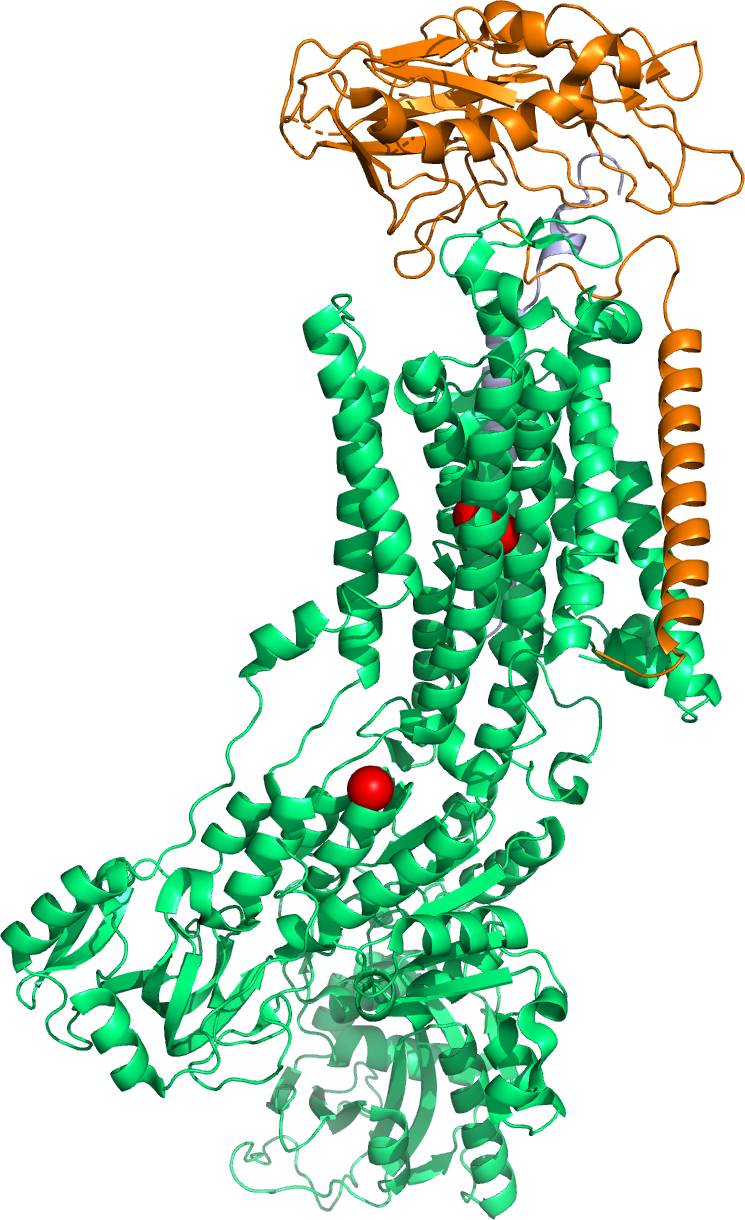
\includegraphics[width=0.7\linewidth]{./figures/potential/Na_K_pump} 

}

\caption{A cartoon representation of the molecular structure of the sodium - potassium pump based on atomic coordinates of \href{https://www.rcsb.org/structure/2ZXE}{PDB 2ZXE}, rendered with open source molecular visualization tool PyMol.}\label{fig:nakpump}
\end{figure}

If the numbers of each type of ion were equal, the sodium--potassium pump would be electrically neutral, but, because of the three-for-two exchange, it gives a net movement of one positive charge from intracellular to extracellular for each cycle, thereby contributing to a positive voltage difference. The pump has three effects: (1) it makes the sodium concentration high in the extracellular space and low in the intracellular space; (2) it makes the potassium concentration high in the intracellular space and low in the extracellular space; (3) it gives the intracellular space a negative voltage with respect to the extracellular space.

The sodium-potassium pump is relatively slow in operation. If a cell were initialized with equal concentrations of sodium and potassium everywhere, it would take hours for the pump to establish equilibrium. The pump operates constantly, but becomes progressively less efficient as the concentrations of sodium and potassium available for pumping are reduced.

Ion pumps influence the action potential only by establishing the relative ratio of intracellular and extracellular ion concentrations. The action potential involves mainly the opening and closing of ion channels not ion pumps. If the ion pumps are turned off by removing their energy source, or by adding an inhibitor such as ouabain, the axon can still fire hundreds of thousands of action potentials before their amplitudes begin to decay significantly. In particular, ion pumps play no significant role in the repolarization of the membrane after an action potential.

Another functionally important ion pump is the sodium-calcium exchanger. This pump operates in a conceptually similar way to the sodium-potassium pump, except that in each cycle it exchanges three Na\textsuperscript{+} from the extracellular space for one Ca\textsuperscript{2+} from the intracellular space. Because the net flow of charge is inward, this pump runs ``downhill'', in effect, and therefore does not require any energy source except the membrane voltage. Its most important effect is to pump calcium outward---it also allows an inward flow of sodium, thereby counteracting the sodium-potassium pump, but, because overall sodium and potassium concentrations are much higher than calcium concentrations, this effect is relatively unimportant. The net result of the sodium-calcium exchanger is that in the resting state, intracellular calcium concentrations become very low.

\hypertarget{ion-channels}{%
\subsection{Ion Channels}\label{ion-channels}}

Ion channels are integral membrane proteins with a pore through which ions can travel between extracellular space and cell interior. Most channels are specific (selective) for one ion; for example, most potassium channels are characterized by 1000:1 selectivity ratio for potassium over sodium, though potassium and sodium ions have the same charge and differ only slightly in their radius. The channel pore is typically so small that ions must pass through it in single-file order. Channel pores can be either open or closed for ion passage, although a number of channels demonstrate various sub-conductance levels. When a channel is open, ions permeate through the channel pore down the transmembrane concentration gradient for that particular ion. Rate of ionic flow through the channel, i.e.~single-channel current amplitude, is determined by the maximum channel conductance and electrochemical driving force for that ion, which is the difference between the instantaneous value of the membrane potential and the value of the reversal potential.

The fundamental properties of currents mediated by ion channels were analyzed by the British biophysicists \href{https://en.wikipedia.org/wiki/Alan_Hodgkin}{Alan Hodgkin} and \href{https://en.wikipedia.org/wiki/Andrew_Huxley}{Andrew Huxley} as part of their Nobel Prize-winning research on the action potential, published in 1952. They built on the work of other physiologists, such as \href{https://en.wikipedia.org/wiki/Kenneth_Stewart_Cole}{Kenneth Stewart Cole's} research into voltage-gated membrane pores from 1941. The existence of ion channels was confirmed in the 1970s by \href{https://en.wikipedia.org/wiki/Bernard_Katz}{Bernard Katz} and \href{https://en.wikipedia.org/wiki/Ricardo_Miledi}{Ricardo Miledi} using noise analysis. It was then shown more directly with an electrical recording technique known as the ``patch clamp'', which led to a Nobel Prize to \href{https://en.wikipedia.org/wiki/Erwin_Neher}{Erwin Neher} and \href{https://en.wikipedia.org/wiki/Bert_Sakmann}{Bert Sakmann}, the technique's inventors. Hundreds if not thousands of researchers continue to pursue a more detailed understanding of how these proteins work.

Channels differ with respect to the ion they let pass (for example, Na\textsuperscript{+}, K\textsuperscript{+}, Cl\textsuperscript{−}), the ways in which they may be regulated, the number of subunits of which they are composed and other aspects of structure. Channels belonging to the largest class, which includes the voltage-gated channels that underlie the nerve impulse, consists of four subunits with six transmembrane helices each. On activation, these helices move about and open the pore. Two of these six helices are separated by a loop that lines the pore and is the primary determinant of ion selectivity and conductance in this channel class and some others. The existence and mechanism for ion selectivity was first postulated in the late 1960s by \href{https://en.wikipedia.org/wiki/Bertil_Hille}{Bertil Hille} and \href{https://en.wikipedia.org/wiki/Clay_Armstrong}{Clay Armstrong}. The idea of the ionic selectivity for potassium channels was that the carbonyl oxygens of the protein backbones of the ``selectivity filter'' (named by Bertil Hille) could efficiently replace the water molecules that normally shield potassium ions, but that sodium ions were smaller and cannot be completely dehydrated to allow such shielding, and therefore could not pass through. This mechanism was finally confirmed when the first structure of an ion channel was elucidated. A bacterial potassium channel KcsA, consisting of just the selectivity filter, ``P'' loop and two transmembrane helices was used as a model to study the permeability and the selectivity of ion channels. The determination of the molecular structure of KcsA by \href{https://en.wikipedia.org/wiki/Roderick_MacKinnon}{Roderick MacKinnon} using X-ray crystallography won a share of the 2003 Nobel Prize in Chemistry.



\begin{figure}

{\centering 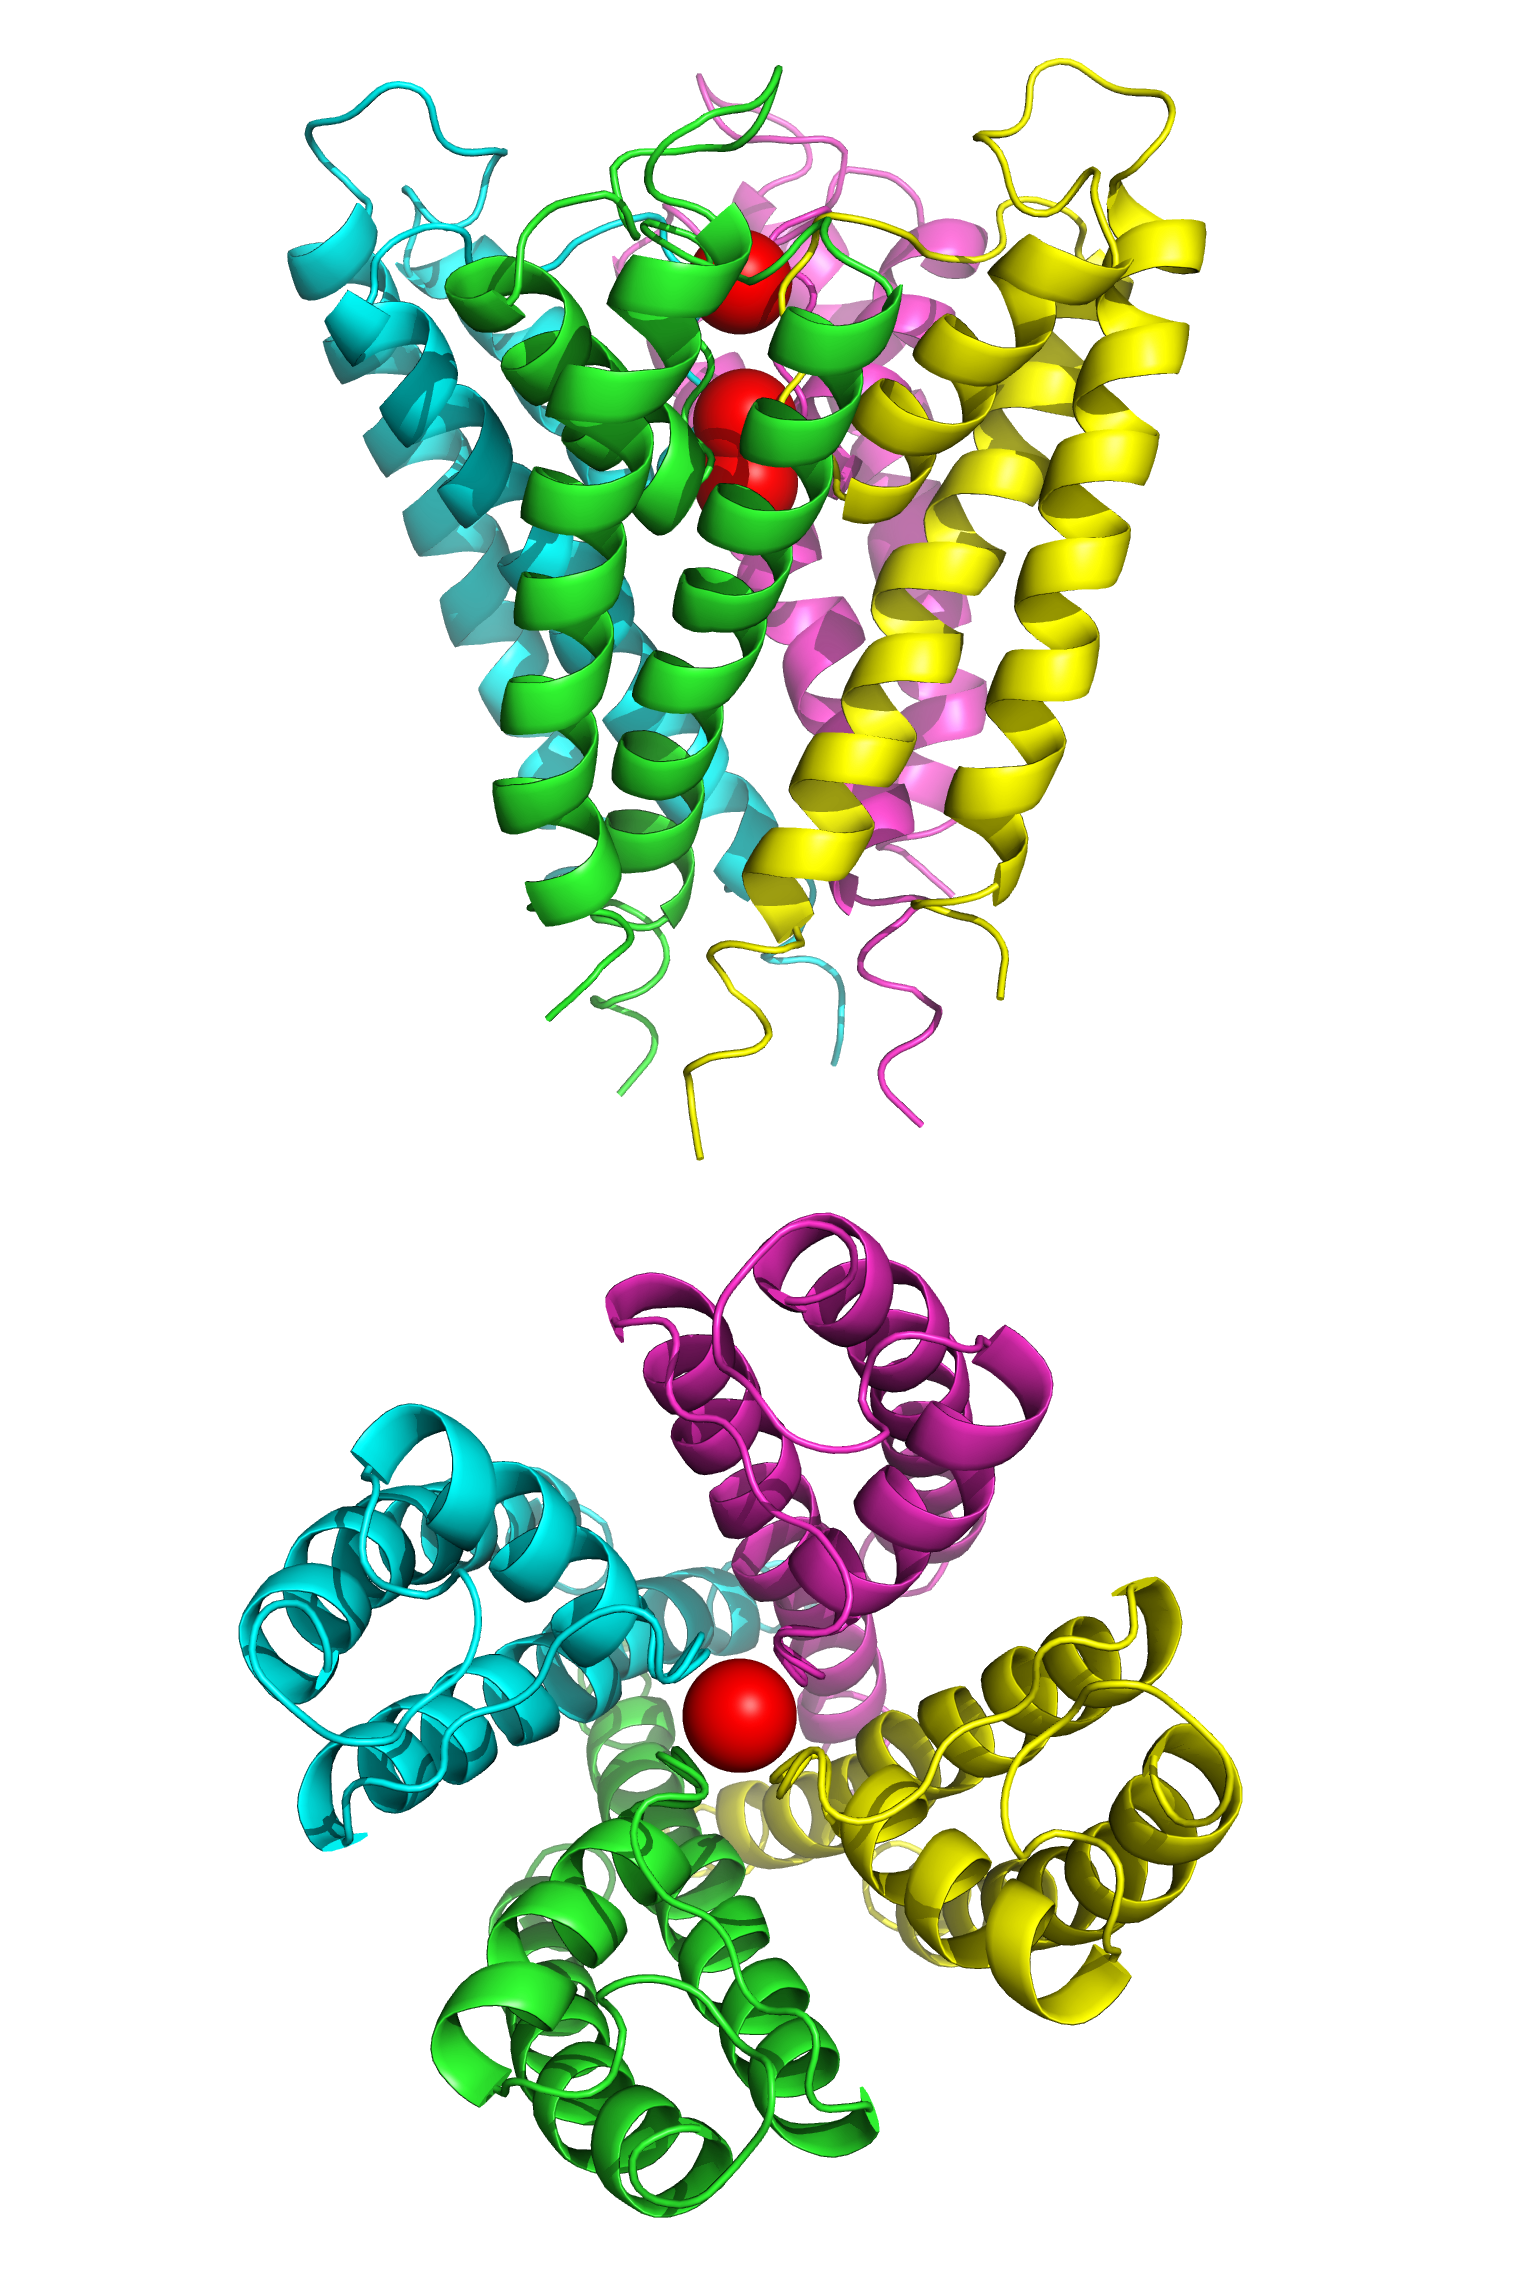
\includegraphics[width=0.7\linewidth]{./figures/potential/Kcsa} 

}

\caption{The structure of the potassium channel KcsA fromn \emph{Streptomyces lividans} determined by X-ray crystallography.Top: side view; bottom: top view. KcsA shares sequence similarity with all known K\textsuperscript{+} channels and was the first ion channel to have its structure solved at atomic resolution. It consists of four identical subunits that together form a cone shaped structure (top) with a ion selectivity filter at its outer end. Three K\textsuperscript{+} ions (red spheres) are present in the channel, two of which are held 7.5 angstroms apart by the selectivity filter, a third K\textsuperscript{+} ion shown in the channel pore below. Data from \href{https://www.rcsb.org/structure/1BL8}{PDB 1BL8}, rendered with open source molecular visualization tool \href{https://pymol.org/2/}{PyMol}.}\label{fig:kchannel}
\end{figure}

Because of their small size and the difficulty of crystallizing integral membrane proteins for X-ray analysis, it is only very recently that scientists have been able to directly examine what channels ``look like.'' Most of what researchers have deduced about channel operation so far they have established through electrophysiology, biochemistry, gene sequence comparison and mutagenesisi and structural studies (X-ray crystallography and cryoelectronmicroscopy).

Channels can have single (e.g.~members of the Chloride Intracellular Ion Channel family) or multiple transmembrane (K\textsuperscript{+} channels, P2X receptors, Na\textsuperscript{+} channels) domains which span the plasma membrane to form pores.

Ion channels can be classified by how they respond to their environment. For example, the ion channels involved in the action potential are voltage-sensitive channels; they open and close in response to the voltage across the membrane. Ligand-gated channels form another important class; these ion channels open and close in response to the binding of a ligand molecule, such as a neurotransmitter. Other ion channels open and close with mechanical forces. Still other ion channels---such as those of sensory neurons---open and close in response to other stimuli, such as light, temperature or pressure.

Leakage channels are the simplest type of ion channel, in that their permeability is more or less constant. The types of leakage channels that have the greatest significance in neurons are potassium and chloride channels. Even these are not perfectly constant in their properties: First, most of them are voltage-dependent in the sense that they conduct better in one direction than the other (in other words, they are rectifiers); second, some of them are capable of being shut off by chemical ligands even though they do not require ligands in order to operate.

\href{https://en.wikipedia.org/wiki/Voltage-gated_ion_channel}{Voltage-gated ion channels} are a class of transmembrane proteins that form ion channels that are activated by changes in the electrical membrane potential near the channel. The membrane potential alters the conformation of the channel proteins, regulating their opening and closing. Cell membranes are generally impermeable to ions, thus they must diffuse through the membrane through transmembrane protein channels. They have a crucial role in excitable cells such as neuronal and muscle tissues, allowing a rapid and co-ordinated depolarization in response to triggering voltage change. Found along the axon and at the synapse, voltage-gated ion channels directionally propagate electrical signals. Voltage-gated ion-channels are usually ion-specific, and channels specific to sodium (Na\textsuperscript{+}), potassium (K\textsuperscript{+}), calcium (Ca\textsuperscript{2+}), and chloride (Cl−) ions have been identified. The opening and closing of the channels are triggered by changing ion concentration, and hence charge gradient, between the sides of the cell membrane.

Voltage-gated ion channels are generally composed of several subunits arranged in such a way that there is a central pore through which ions can travel down their electrochemical gradients. The channels tend to be ion-specific, although similarly sized and charged ions may sometimes travel through them. The functionality of voltage-gated ion channels is attributed to its three main discrete units: the voltage sensor, the pore or conducting pathway, and the gate. Na\textsuperscript{+}, K\textsuperscript{+}, and Ca\textsuperscript{2+} channels are composed of four transmembrane domains arranged around a central pore; these four domains are part of a single α-subunit in the case of most Na\textsuperscript{+} and Ca\textsuperscript{2+} channels, whereas there are four α-subunits, each contributing one transmembrane domain, in most K\textsuperscript{+} channels. The membrane-spanning segments, designated S1-S6, all take the form of alpha helices with specialized functions. The fifth and sixth transmembrane segments (S5 and S6) and pore loop serve the principal role of ion conduction, comprising the gate and pore of the channel, while S1-S4 serve as the voltage-sensing region. The four subunits may be identical, or different from one another. In addition to the four central α-subunits, there are also regulatory β-subunits, with oxidoreductase activity, which are located on the inner surface of the cell membrane and do not cross the membrane, and which are coassembled with the α-subunits in the endoplasmic reticulum.

Crystallographic structural studies of a potassium channel have shown that, when a potential difference is introduced over the membrane, the associated electric field induces a conformational change in the potassium channel. The conformational change distorts the shape of the channel proteins sufficiently such that the cavity, or channel, opens to allow influx or efflux to occur across the membrane. This movement of ions down their concentration gradients subsequently generates an electric current sufficient to depolarize the cell membrane.

Voltage-gated sodium channels and calcium channels are made up of a single polypeptide with four homologous domains. Each domain contains 6 membrane spanning alpha helices. One of these helices, S4, is the voltage sensing helix. The S4 segment contains many positive charges such that a high positive charge outside the cell repels the helix, keeping the channel in its closed state.

In general, the voltage sensing portion of the ion channel is responsible for the detection of changes in transmembrane potential that trigger the opening or closing of the channel. The S1-4 alpha helices are generally thought to serve this role. In potassium and sodium channels, voltage-sensing S4 helices contain positively-charged lysine or arginine residues in repeated motifs. In its resting state, half of each S4 helix is in contact with the cell cytosol. Upon depolarization, the positively-charged residues on the S4 domains move toward the exoplasmic surface of the membrane. It is thought that the first 4 arginines account for the gating current, moving toward the extracellular solvent upon channel activation in response to membrane depolarization. The movement of 10--12 of these protein-bound positive charges triggers a conformational change that opens the channel. The exact mechanism by which this movement occurs is not currently agreed upon, however the canonical, transporter, paddle, and twisted models are examples of current theories.

Movement of the voltage-sensor triggers a conformational change of the gate of the conducting pathway, controlling the flow of ions through the channel.

The main functional part of the voltage-sensitive protein domain of these channels generally contains a region composed of S3b and S4 helices, known as the ``paddle'' due to its shape, which appears to be a conserved sequence, interchangeable across a wide variety of cells and species. A similar voltage sensor paddle has also been found in a family of voltage sensitive phosphatases in various species. Genetic engineering of the paddle region from a species of volcano-dwelling archaebacteria into rat brain potassium channels results in a fully functional ion channel, as long as the whole intact paddle is replaced. This ``modularity'' allows use of simple and inexpensive model systems to study the function of this region, its role in disease, and pharmaceutical control of its behavior rather than being limited to poorly characterized, expensive, and/or difficult to study preparations.

Although voltage-gated ion channels are typically activated by membrane depolarization, some channels, such as inward-rectifier potassium ion channels, are activated instead by hyperpolarization.

The gate is thought to be coupled to the voltage sensing regions of the channels and appears to contain a mechanical obstruction to ion flow. While the S6 domain has been agreed upon as the segment acting as this obstruction, its exact mechanism is unknown. Possible explanations include: the S6 segment makes a scissor-like movement allowing ions to flow through, the S6 segment breaks into two segments allowing of passing of ions through the channel, or the S6 channel serving as the gate itself. The mechanism by which the movement of the S4 segment affects that of S6 is still unknown, however it is theorized that there is a S4-S5 linker whose movement allows the opening of S6.

Inactivation of ion channels occurs within milliseconds after opening. Inactivation is thought to be mediated by an intracellular gate that controls the opening of the pore on the inside of the cell. This gate is modeled as a ball tethered to a flexible chain. During inactivation, the chain folds in on itself and the ball blocks the flow of ions through the channel. Fast inactivation is directly linked to the activation caused by intramembrane movements of the S4 segments, though the mechanism linking movement of S4 and the engagement of the inactivation gate is unknown.

Important representative families of voltage-gated ion channels are the:

\begin{itemize}
\tightlist
\item
  Voltage-gated sodium channels: This family contains at least 9 members and is largely responsible for action potential creation and propagation. The pore-forming α subunits are very large (up to 4,000 amino acids) and consist of four homologous repeat domains (I-IV) each comprising six transmembrane segments (S1-S6) for a total of 24 transmembrane segments. The members of this family also coassemble with auxiliary β subunits, each spanning the membrane once. Both α and β subunits are extensively glycosylated.
\item
  Voltage-gated calcium channels: This family consists of channels that are formed as a complex of several different subunits: α1, α2δ, β1-4, and γ. The α1 subunit forms the Ca\textsuperscript{2+} selective ion conducting pore while the associated subunits have several functions including modulation of gating.These channels play an important role in both linking muscle excitation with contraction as well as neuronal excitation with transmitter release. The α subunits have an overall structural resemblance to those of the sodium channels and are equally large.
\item
  Cation channels of sperm: This small family of channels, normally referred to as Catsper channels, is related to the two-pore channels and distantly related to TRP channels.
\item
  Voltage-gated potassium channels (KV): This family contains almost 40 members, which are further divided into 12 subfamilies. These channels are known mainly for their role in repolarizing the cell membrane following action potentials. The α subunits have six transmembrane segments, homologous to a single domain of the sodium channels. Correspondingly, they assemble as tetramers to produce a functioning channel.
\item
  Some transient receptor potential channels: This group of channels, normally referred to simply as TRP channels, is named after their role in \emph{Drosophila} phototransduction. This family, containing at least 28 members, is incredibly diverse in its method of activation. Some TRP channels seem to be constitutively open, while others are gated by voltage, intracellular Ca\textsuperscript{2+}, pH, redox state, osmolarity, and mechanical stretch. These channels also vary according to the ion(s) they pass, some being selective for Ca\textsuperscript{2+} while others are less selective, acting as cation channels. This family is subdivided into 6 subfamilies based on homology: classical (TRPC), vanilloid receptors (TRPV), melastatin (TRPM), polycystins (TRPP), mucolipins (TRPML), and ankyrin transmembrane protein 1 (TRPA).
\item
  Hyperpolarization-activated cyclic nucleotide-gated channels: The opening of these channels is due to hyperpolarization rather than the depolarization required for other cyclic nucleotide-gated channels. These channels are also sensitive to the cyclic nucleotides cAMP and cGMP, which alter the voltage sensitivity of the channel's opening. These channels are permeable to the monovalent cations K\textsuperscript{+} and Na\textsuperscript{+}. There are 4 members of this family, all of which form tetramers of six-transmembrane α subunits. As these channels open under hyperpolarizing conditions, they function as pacemaking channels in the heart, particularly the SA node.
\item
  Voltage-gated proton channels: Voltage-gated proton channels open with depolarization, but in a strongly pH-sensitive manner. The result is that these channels open only when the electrochemical gradient is outward, such that their opening will only allow protons to leave cells. Their function thus appears to be acid extrusion from cells. Another important function occurs in phagocytes (e.g.~eosinophils, neutrophils, macrophages) during the ``respiratory burst.'' When bacteria or other microbes are engulfed by phagocytes, the enzyme NADPH oxidase assembles in the membrane and begins to produce reactive oxygen species (ROS) that help kill bacteria. NADPH oxidase is electrogenic, moving electrons across the membrane, and proton channels open to allow proton flux to balance the electron movement electrically.
\end{itemize}



\begin{figure}

{\centering \includegraphics[width=0.7\linewidth]{./figures/potential/voltage_gated_ion_channels} 

}

\caption{The structures (from left to right) of voltage-gated sodium, potassium, calcium and chloride channels. Top: side view; bottom: top view. Data from \href{https://www.rcsb.org/structure/5EK0}{PDB 5EK0}, \href{https://www.rcsb.org/structure/2A79}{PDB 2A79}, \href{https://www.rcsb.org/structure/3JBR}{PDB 3JBR} and \href{https://www.rcsb.org/structure/1KPL}{PDB 1KPL} rendered with open source molecular visualization tool \href{https://pymol.org/2/}{PyMol}.}\label{fig:ionchannel}
\end{figure}

\href{https://en.wikipedia.org/wiki/Ligand-gated_ion_channel}{Ligand-gated ion channels}, also commonly referred to as ionotropic receptors, are a group of transmembrane ion-channel proteins which open to allow ions such as Na\textsuperscript{+}, K\textsuperscript{+}, Ca\textsuperscript{2+}, and Cl\textsuperscript{−} to pass through the membrane in response to the binding of a chemical messenger (i.e.~a ligand), such as a neurotransmitter.

When a presynaptic neuron is excited, it releases a neurotransmitter from vesicles into the synaptic cleft. The neurotransmitter then binds to receptors located on the postsynaptic neuron. If these receptors are ligand-gated ion channels, a resulting conformational change opens the ion channels, which leads to a flow of ions across the cell membrane. This, in turn, results in either a depolarization, for an excitatory receptor response, or a hyperpolarization, for an inhibitory response.

These receptor proteins are typically composed of at least two different domains: a transmembrane domain which includes the ion pore, and an extracellular domain which includes the ligand binding location (an allosteric binding site). This modularity has enabled a `divide and conquer' approach to finding the structure of the proteins (crystallising each domain separately). The function of such receptors located at synapses is to convert the chemical signal of presynaptically released neurotransmitter directly and very quickly into a postsynaptic electrical signal. Many ligand-gated ion channels are additionally modulated by allosteric ligands, by channel blockers, ions, or the membrane potential. Ligand-gated ion channels are classified into three superfamilies which lack evolutionary relationship: cys-loop receptors, ionotropic glutamate receptors and ATP-gated channels.

The cys-loop receptors are named after a characteristic loop formed by a disulfide bond between two cysteine residues in the N terminal extracellular domain. They are part of a larger family of pentameric ligand-gated ion channels that usually lack this disulfide bond, hence the tentative name ``Pro-loop receptors''. A binding site in the extracellular N-terminal ligand-binding domain gives them receptor specificity for (1) acetylcholine (AcCh), (2) serotonin, (3) glycine, (4) glutamate and (5) γ-aminobutyric acid (GABA) in vertebrates. The receptors are subdivided with respect to the type of ion that they conduct (anionic or cationic) and further into families defined by the endogenous ligand. They are usually pentameric with each subunit containing 4 transmembrane helices constituting the transmembrane domain, and a beta sheet sandwich type, extracellular, N terminal, ligand binding domain. Some also contain an intracellular domain like shown in the image.

The prototypic ligand-gated ion channel is the nicotinic acetylcholine receptor. It consists of a pentamer of protein subunits (typically ααβγδ), with two binding sites for acetylcholine (one at the interface of each alpha subunit). When the acetylcholine binds it alters the receptor's configuration (twists the T2 helices which moves the leucine residues, which block the pore, out of the channel pathway) and causes the constriction in the pore of approximately 3 angstroms to widen to approximately 8 angstroms so that ions can pass through. This pore allows Na\textsuperscript{+} ions to flow down their electrochemical gradient into the cell. With a sufficient number of channels opening at once, the inward flow of positive charges carried by Na\textsuperscript{+} ions depolarizes the postsynaptic membrane sufficiently to initiate an action potential.

While single-cell organisms like bacteria would have little apparent need for the transmission of an action potential, a bacterial homologue to an LIC has been identified, hypothesized to act nonetheless as a chemoreceptor. This prokaryotic nAChR variant is known as the GLIC receptor, after the species in which it was identified; Gloeobacter Ligand-gated Ion C channel.

The ionotropic glutamate receptors bind the neurotransmitter glutamate. They form tetramers with each subunit consisting of an extracellular amino terminal domain (ATD, which is involved tetramer assembly), an extracellular ligand binding domain (LBD, which binds glutamate), and a transmembrane domain (TMD, which forms the ion channel). The transmembrane domain of each subunit contains three transmembrane helices as well as a half membrane helix with a reentrant loop. The structure of the protein starts with the ATD at the N terminus followed by the first half of the LBD which is interrupted by helices 1,2 and 3 of the TMD before continuing with the final half of the LBD and then finishing with helix 4 of the TMD at the C terminus. This means there are three links between the TMD and the extracellular domains. Each subunit of the tetramer has a binding site for glutamate formed by the two LBD sections forming a clamshell like shape. Only two of these sites in the tetramer need to be occupied to open the ion channel. The pore is mainly formed by the half helix 2 in a way which resembles an inverted potassium channel.



\begin{figure}

{\centering \includegraphics[width=0.7\linewidth]{./figures/potential/ligand_gated_ion_channels} 

}

\caption{Structures of ligand-gated ion channels. Top row: The nicotinic acetylcholine receptor (left) and the serotonin 5-HT3 receptor. Middle row: The GABA\textsubscript{A} receptor (left) and glycine receptor (rigt). Bottom row: The AMPA receptor (left) and NMDA receptor (reight). Data from \href{https://www.rcsb.org/structure/2BG9}{PDB 2BG9}, \href{https://www.rcsb.org/structure/6HIO}{PDB 6HIO}, \href{https://www.rcsb.org/structure/6D6U}{PDB 6D6U}, \href{https://www.rcsb.org/structure/3JAD}{PDB 3JAD}, \href{https://www.rcsb.org/structure/5IDE}{PDB 5IDE}, and \href{https://www.rcsb.org/structure/4PE5}{PDB 4PE5}, rendered with open source molecular visualization tool \href{https://pymol.org/2/}{PyMol}.}\label{fig:lgic}
\end{figure}

Also called G protein-coupled receptor, seven-transmembrane domain receptor, 7 TM receptor, constitute a large protein family of receptors that sense molecules outside the cell and activate inside signal transduction pathways and, ultimately, cellular responses. They pass through the cell membrane 7 times. G-protein-Linked receptors are a huge family that have hundreds of members identified. Ion-channel-linked receptors (e.g.~GABAB, NMDA, etc.) are only a part of them.

\hypertarget{the-reversal-potential}{%
\subsection{The Reversal Potential}\label{the-reversal-potential}}

The reversal potential (or equilibrium potential) of an ion is the value of transmembrane voltage at which diffusive and electrical forces counterbalance, so that there is no net ion flow across the membrane. This means that the transmembrane voltage exactly opposes the force of diffusion of the ion, such that the net current of the ion across the membrane is zero and unchanging. The reversal potential is important because it corresponds to the voltage that acts on channels permeable to that ion---in other words, it gives the voltage that the ion concentration gradient generates when it acts as a battery.

The equilibrium potential of a particular ion is usually designated by the notation E\textsubscript{ion}.The equilibrium potential for any ion can be calculated using the Nernst equation. For example, reversal potential for potassium ions will be as follows:

\[  E_{eq,K^+} = \frac{RT}{zF} \ln \frac{[K^+]_{o}}{[K^+]_{i}} \]

where

\begin{itemize}
\tightlist
\item
  E\textsubscript{eq,K\textsuperscript{+}} is the equilibrium potential for potassium, measured in volts
\item
  R is the universal gas constant, equal to 8.314 Joule·K\textsuperscript{−1}·mol\textsuperscript{−1}
\item
  T is the absolute temperature, measured in Kelvin
\item
  z is the number of elementary charges of the ion in question involved in the reaction
\item
  F is the Faraday constant, equal to 96,485 Coulomb·mol\textsuperscript{−1} or J·V\textsuperscript{−1}·mol\textsuperscript{−1}
\item
  {[}K\textsuperscript{+}{]}\textsubscript{o} is the extracellular concentration of potassium, measured in mol·m\textsuperscript{−3} or mmol·l\textsuperscript{−1}
\item
  {[}K\textsuperscript{+}{]}\textsubscript{i} is the intracellular concentration of potassium
\end{itemize}

Even if two different ions have the same charge (i.e., K\textsuperscript{+} and Na\textsuperscript{+}), they can still have very different equilibrium potentials, provided their outside and/or inside concentrations differ. Take, for example, the equilibrium potentials of potassium and sodium in neurons. The potassium equilibrium potential E\textsubscript{K} is −84 mV with 5 mM potassium outside and 140 mM inside. On the other hand, the sodium equilibrium potential, E\textsubscript{Na}, is approximately +66 mV with approximately 12 mM sodium inside and 140 mM outside.

A neuron's resting membrane potential actually changes during the development of an organism. In order for a neuron to eventually adopt its full adult function, its potential must be tightly regulated during development. As an organism progresses through development the resting membrane potential becomes more negative. Glial cells are also differentiating and proliferating as development progresses in the brain. The addition of these glial cells increases the organism's ability to regulate extracellular potassium. The drop in extracellular potassium can lead to a decrease in membrane potential of 35 mV.

Cell excitability is the change in membrane potential that is necessary for cellular responses in various tissues. Cell excitability is a property that is induced during early embriogenesis. Excitability of a cell has also been defined as the ease with which a response may be triggered. The resting potential forms the basis of cell excitability and these processes are fundamental for the generation of graded and action potentials.

The most important regulators of cell excitability are the extracellular calcium concentration and the calcium-sensing receptor. Calcium is also the most important second messenger in excitable cell signaling. Other important proteins that regulate cell excitability are voltage-gated ion channels, ion transporters, membrane receptors and hyperpolarization-activated cyclic-nucleotide-gated channels. For example, potassium channels are important regulators of excitability in neurons, cardiac myocytes and many other excitable cells like astrocytes. Activation of synaptic receptors initiates long-lasting changes in neuronal excitability.

Many cell types are considered to have an excitable membrane. Excitable cells are neurons, cardiac myocytes, skeletal myocytes, smooth muscle cells, many types of endothelial cells (e.g.~beta cells), glial cells (e.g.~astrocytes), mechanoreceptor cells (e.g.~hair cells and Merkel cells), chemoreceptor cells (e.g.~glomus cells, taste receptors), some plant cells and possibly immune cells. Astrocytes display a form of non-electrical excitability based on intracellular calcium variations related to the expression of several receptors through which they can detect the synaptic signal. In neurons, there are different membrane properties in some portions of the cell, for example, dendritic excitability endows neurons with the capacity for coincidence detection of spatially separated inputs.

\hypertarget{the-resting-potential}{%
\subsection{The Resting Potential}\label{the-resting-potential}}

When the membrane potential of a cell goes for a long period of time without changing significantly, it is referred to as a resting potential or resting voltage. This term is used for the membrane potential of non-excitable cells, but also for the membrane potential of excitable cells in the absence of excitation. In excitable cells, the other possible states are graded membrane potentials (of variable amplitude), and action potentials, which are large, all-or-nothing rises in membrane potential that usually follow a fixed time course. Excitable cells include neurons, muscle cells, and some secretory cells in glands. Even in other types of cells, however, the membrane voltage can undergo changes in response to environmental or intracellular stimuli. For example, depolarization of the plasma membrane appears to be an important step in programmed cell death.

The interactions that generate the resting potential are modeled by the Goldman equation. This is similar in form to the Nernst equation shown above, in that it is based on the charges of the ions in question, as well as the difference between their inside and outside concentrations. However, it also takes into consideration the relative permeability of the plasma membrane to each ion in question.

\[ E_{m} = \frac{RT}{F} \ln{ \left( \frac{ P_{\mathrm{K}}[\mathrm{K}^{+}]_\mathrm{out} + P_{\mathrm{Na}}[\mathrm{Na}^{+}]_\mathrm{out} + P_{\mathrm{Cl}}[\mathrm{Cl}^{-}]_\mathrm{in}}{ P_{\mathrm{K}}[\mathrm{K}^{+}]_\mathrm{in} + P_{\mathrm{Na}}[\mathrm{Na}^{+}]_\mathrm{in} + P_{\mathrm{Cl}}[\mathrm{Cl}^{-}]_\mathrm{out}} \right) } \]

The three ions that appear in this equation are potassium (K\textsuperscript{+}), sodium (Na\textsuperscript{+}), and chloride (Cl\textsuperscript{−}). Calcium is omitted, but can be added to deal with situations in which it plays a significant role. Being an anion, the chloride terms are treated differently from the cation terms; the intracellular concentration is in the numerator, and the extracellular concentration in the denominator, which is reversed from the cation terms. \emph{P\textsubscript{i}} stands for the relative permeability of the ion type \emph{i}.

In essence, the Goldman formula expresses the membrane potential as a weighted average of the reversal potentials for the individual ion types, weighted by permeability. (Although the membrane potential changes about 100 mV during an action potential, the concentrations of ions inside and outside the cell do not change significantly. They remain close to their respective concentrations when the membrane is at resting potential.) In most animal cells, the permeability to potassium is much higher in the resting state than the permeability to sodium. As a consequence, the resting potential is usually close to the potassium reversal potential. The permeability to chloride can be high enough to be significant, but, unlike the other ions, chloride is not actively pumped, and therefore equilibrates at a reversal potential very close to the resting potential determined by the other ions.

Values of resting membrane potential in most animal cells usually vary between the potassium reversal potential (usually around -80 mV) and around -40 mV. The resting potential in excitable cells (capable of producing action potentials) is usually near -60 mV---more depolarized voltages would lead to spontaneous generation of action potentials. Immature or undifferentiated cells show highly variable values of resting voltage, usually significantly more positive than in differentiated cells. In such cells, the resting potential value correlates with the degree of differentiation: undifferentiated cells in some cases may not show any transmembrane voltage difference at all.

Maintenance of the resting potential can be metabolically costly for a cell because of its requirement for active pumping of ions to counteract losses due to leakage channels. The cost is highest when the cell function requires an especially depolarized value of membrane voltage. For example, the resting potential in daylight-adapted blowfly (\emph{Calliphora vicina}) photoreceptors can be as high as -30 mV. This elevated membrane potential allows the cells to respond very rapidly to visual inputs; the cost is that maintenance of the resting potential may consume more than 20\% of overall cellular ATP.

On the other hand, the high resting potential in undifferentiated cells can be a metabolic advantage. This apparent paradox is resolved by examination of the origin of that resting potential. Little-differentiated cells are characterized by extremely high input resistance, which implies that few leakage channels are present at this stage of cell life. As an apparent result, potassium permeability becomes similar to that for sodium ions, which places resting potential in-between the reversal potentials for sodium and potassium as discussed above. The reduced leakage currents also mean there is little need for active pumping in order to compensate, therefore low metabolic cost.

\hypertarget{the-action-potential}{%
\subsection{The Action Potential}\label{the-action-potential}}

An action potential occurs when the membrane potential of a specific cell location rapidly rises and falls: this depolarisation then causes adjacent locations to similarly depolarise. Action potentials occur in several types of animal cells, called excitable cells, which include neurons, muscle cells, endocrine cells, glomus cells (peripheral chemoreceptor cells mainly located in the carotid and aortic bodies), and in some plant cells.

In neurons, action potentials play a central role in cell-to-cell communication by providing for---or with regard to saltatory conduction, assisting---the propagation of signals along the neuron's axon toward synaptic boutons situated at the ends of an axon; these signals can then connect with other neurons at synapses, or to motor cells or glands. In other types of cells, their main function is to activate intracellular processes. In muscle cells, for example, an action potential is the first step in the chain of events leading to contraction. In beta cells of the pancreas, they provoke release of insulin. Action potentials in neurons are also known as ``nerve impulses'' or ``spikes'', and the temporal sequence of action potentials generated by a neuron is called its ``spike train''. A neuron that emits an action potential, or nerve impulse, is often said to ``fire''.

Action potentials are generated by special types of voltage-gated ion channels embedded in a cell's plasma membrane. These channels are shut when the membrane potential is near the (negative) resting potential of the cell, but they rapidly begin to open if the membrane potential increases to a precisely defined threshold voltage, depolarising the transmembrane potential. When the channels open, they allow an inward flow of sodium ions, which changes the electrochemical gradient, which in turn produces a further rise in the membrane potential. This then causes more channels to open, producing a greater electric current across the cell membrane and so on. The process proceeds explosively until all of the available ion channels are open, resulting in a large upswing in the membrane potential. The rapid influx of sodium ions causes the polarity of the plasma membrane to reverse, and the ion channels then rapidly inactivate. As the sodium channels close, sodium ions can no longer enter the neuron, and they are then actively transported back out of the plasma membrane. Potassium channels are then activated, and there is an outward current of potassium ions, returning the electrochemical gradient to the resting state. After an action potential has occurred, there is a transient negative shift, called the afterhyperpolarization.

In animal cells, there are two primary types of action potentials. One type is generated by voltage-gated sodium channels, the other by voltage-gated calcium channels. Sodium-based action potentials usually last for under one millisecond, but calcium-based action potentials may last for 100 milliseconds or longer. In some types of neurons, slow calcium spikes provide the driving force for a long burst of rapidly emitted sodium spikes. In cardiac muscle cells, on the other hand, an initial fast sodium spike provides a ``primer'' to provoke the rapid onset of a calcium spike, which then produces muscle contraction



\begin{figure}

{\centering 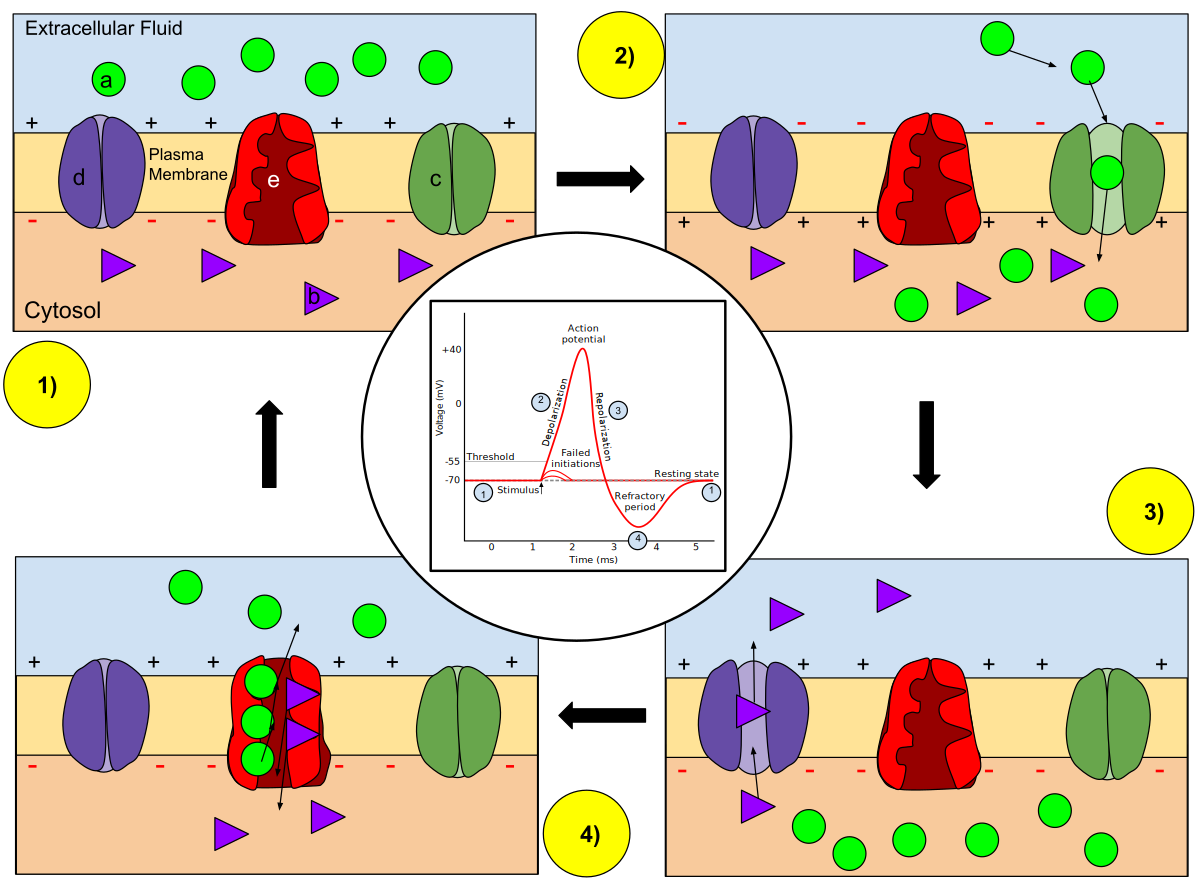
\includegraphics[width=0.7\linewidth]{./figures/potential/ActionPotential} 

}

\caption{\href{https://commons.wikimedia.org/wiki/File:Membrane_Permeability_of_a_Neuron_During_an_Action_Potential.svg}{Ion movement during an action potential.} Key: a) Sodium (Na\textsuperscript{+}) ion. b) Potassium (K\textsuperscript{+}) ion. c) Sodium channel. d) Potassium channel. e) Sodium-potassium pump. In the stages of an action potential, the permeability of the membrane of the neuron changes. At the resting state (1), sodium and potassium ions have limited ability to pass through the membrane, and the neuron has a net negative charge inside. Once the action potential is triggered, the depolarization (2) of the neuron activates sodium channels, allowing sodium ions to pass through the cell membrane into the cell, resulting in a net positive charge in the neuron relative to the extracellular fluid. After the action potential peak is reached, the neuron begins repolarization (3), where the sodium channels close and potassium channels open, allowing potassium ions to cross the membrane into the extracellular fluid, returning the membrane potential to a negative value. Finally, there is a refractory period (4), during which the voltage-dependent ion channels are inactivated while the Na\textsuperscript{+} and K\textsuperscript{+} ions return to their resting state distributions across the membrane (1), and the neuron is ready to repeat the process for the next action potential.}\label{fig:actionpotential}
\end{figure}

\hypertarget{graded-potentials}{%
\subsection{Graded Potentials}\label{graded-potentials}}

As explained above, the potential at any point in a cell's membrane is determined by the ion concentration differences between the intracellular and extracellular areas, and by the permeability of the membrane to each type of ion. The ion concentrations do not normally change very quickly (with the exception of Ca\textsuperscript{2+}, where the baseline intracellular concentration is so low that even a small influx may increase it by orders of magnitude), but the permeabilities of the ions can change in a fraction of a millisecond, as a result of activation of ligand-gated ion channels. The change in membrane potential can be either large or small, depending on how many ion channels are activated and what type they are, and can be either long or short, depending on the lengths of time that the channels remain open. Changes of this type are referred to as graded potentials, in contrast to action potentials, which have a fixed amplitude and time course.

As can be derived from the Goldman equation shown above, the effect of increasing the permeability of a membrane to a particular type of ion shifts the membrane potential toward the reversal potential for that ion. Thus, opening Na\textsuperscript{+} channels shifts the membrane potential toward the Na\textsuperscript{+} reversal potential, which is usually around +100 mV. Likewise, opening K\textsuperscript{+} channels shifts the membrane potential toward about --90 mV, and opening Cl\textsuperscript{−} channels shifts it toward about --70 mV (resting potential of most membranes). Thus, Na\textsuperscript{+} channels shift the membrane potential in a positive direction, K\textsuperscript{+} channels shift it in a negative direction (except when the membrane is hyperpolarized to a value more negative than the K\textsuperscript{+} reversal potential), and Cl\textsuperscript{−} channels tend to shift it towards the resting potential.

Graded membrane potentials are particularly important in neurons, where they are produced by synapses---a temporary change in membrane potential produced by activation of a synapse by a single graded or action potential is called a postsynaptic potential. Neurotransmitters that act to open Na\textsuperscript{+} channels typically cause the membrane potential to become more positive, while neurotransmitters that activate K\textsuperscript{+} channels typically cause it to become more negative; those that inhibit these channels tend to have the opposite effect.

Whether a postsynaptic potential is considered excitatory or inhibitory depends on the reversal potential for the ions of that current, and the threshold for the cell to fire an action potential (around --50mV). A postsynaptic current with a reversal potential above threshold, such as a typical Na\textsuperscript{+} current, is considered excitatory. A current with a reversal potential below threshold, such as a typical K\textsuperscript{+} current, is considered inhibitory. A current with a reversal potential above the resting potential, but below threshold, will not by itself elicit action potentials, but will produce subthreshold membrane potential oscillations. Thus, neurotransmitters that act to open Na\textsuperscript{+} channels produce excitatory postsynaptic potentials, or EPSPs, whereas neurotransmitters that act to open K\textsuperscript{+} or Cl\textsuperscript{−} channels typically produce inhibitory postsynaptic potentials, or IPSPs. When multiple types of channels are open within the same time period, their postsynaptic potentials summate (are added together).

From the viewpoint of biophysics, the resting membrane potential is merely the membrane potential that results from the membrane permeabilities that predominate when the cell is resting. The Goldman equation of weighted averages always applies, but the following approach may be more easily visualized. At any given moment, there are two factors for an ion that determine how much influence that ion will have over the membrane potential of a cell:

\begin{enumerate}
\def\labelenumi{\arabic{enumi}.}
\tightlist
\item
  That ion's driving force
\item
  That ion's permeability
\end{enumerate}

If the driving force is high, then the ion is being ``pushed'' across the membrane. If the permeability is high, it will be easier for the ion to diffuse across the membrane.

\begin{itemize}
\tightlist
\item
  Driving force is the net electrical force available to move that ion across the membrane. It is calculated as the difference between the voltage that the ion ``wants'' to be at (its equilibrium potential) and the actual membrane potential (E\textsubscript{m}). So, in formal terms, the driving force for an ion = E\textsubscript{m} - E\textsubscript{ion}
\item
  For example, at our earlier calculated resting potential of −73 mV, the driving force on potassium is 7 mV : (−73 mV) − (−80 mV) = 7 mV. The driving force on sodium would be (−73 mV) − (60 mV) = −133 mV.
\item
  Permeability is a measure of how easily an ion can cross the membrane. It is normally measured as the (electrical) conductance and the unit, siemens (S), corresponds to 1 C·s\textsuperscript{−1}·V\textsuperscript{−1}, that is one coulomb per second per volt of potential.
\end{itemize}

So, in a resting membrane, while the driving force for potassium is low, its permeability is very high. Sodium has a huge driving force but almost no resting permeability. In this case, potassium carries about 20 times more current than sodium, and thus has 20 times more influence over E\textsubscript{m} than does sodium.

However, consider another case---the peak of the action potential. Here, permeability to Na is high and K permeability is relatively low. Thus, the membrane moves to near E\textsubscript{Na} and far from E\textsubscript{K}.

\hypertarget{neurotransmission}{%
\section{Neurotransmission}\label{neurotransmission}}

Neurotransmission (Latin: transmissio ``passage, crossing'' from transmittere ``send, let through'') is the process by which signaling molecules called neurotransmitters are released by the axon terminal of a neuron (the presynaptic neuron), and bind to and react with the receptors on the dendrites of another neuron (the postsynaptic neuron) a short distance away.

Neurotransmission is regulated by several different factors: the availability and rate-of-synthesis of the neurotransmitter, the release of that neurotransmitter, the baseline activity of the postsynaptic cell, the number of available postsynaptic receptors for the neurotransmitter to bind to, and the subsequent removal or deactivation of the neurotransmitter by enzymes or presynaptic reuptake.

In response to a threshold action potential or graded electrical potential, a neurotransmitter is released at the presynaptic terminal. The released neurotransmitter may then move across the synaptic cleft to bind to receptors in the postsynaptic neuron. Binding of neurotransmitters may influence the postsynaptic neuron in either an inhibitory or excitatory way. The binding of neurotransmitters to receptors in the postsynaptic neuron can trigger either short term changes, such as changes in the membrane potential called postsynaptic potentials, or longer term changes by the activation of signaling cascades.

Neurons form complex biological neural networks through which nerve impulses (action potentials) travel. Neurons do not touch each other (except in the case of an electrical synapse through a gap junction); instead, neurons interact at close contact points called synapses. When the nerve impulse arrives at the synapse, it may cause the release of neurotransmitters, which influence another (postsynaptic) neuron. The postsynaptic neuron may receive inputs from many additional neurons, both excitatory and inhibitory. The excitatory and inhibitory influences are summed, and if the net effect is inhibitory, the neuron will be less likely to ``fire'' (i.e., generate an action potential), and if the net effect is excitatory, the neuron will be more likely to fire. How likely a neuron is to fire depends on how far its membrane potential is from the threshold potential, the voltage at which an action potential is triggered because enough voltage-dependent sodium channels are activated so that the net inward sodium current exceeds all outward currents. Excitatory inputs bring a neuron closer to threshold, while inhibitory inputs bring the neuron farther from threshold. An action potential is an ``all-or-none'' event; neurons whose membranes have not reached threshold will not fire, while those that do must fire. Once the action potential is initiated (traditionally at the axon hillock), it will propagate along the axon, leading to release of neurotransmitters at the synaptic bouton to pass along information to yet another adjacent neuron.

Stages in neurotransmission at the synapse

\begin{itemize}
\tightlist
\item
  Synthesis of the neurotransmitter. This can take place in the cell body, in the axon, or in the axon terminal.
\item
  Storage of the neurotransmitter in storage granules or vesicles in the axon terminal.
\item
  Calcium enters the axon terminal during an action potential, causing release of the neurotransmitter into the synaptic cleft.
\item
  After its release, the transmitter binds to and activates a receptor in the postsynaptic membrane.
\item
  Deactivation of the neurotransmitter. The neurotransmitter is either destroyed enzymatically, or taken back into the terminal from which it came, where it can be reused, or degraded and removed.
\end{itemize}

\hypertarget{the-synapse}{%
\subsection{The Synapse}\label{the-synapse}}

In the nervous system, a synapse is a structure that permits a neuron (or nerve cell) to pass an electrical or chemical signal to another neuron or to the target effector cell.

Santiago Ramón y Cajal proposed that neurons are not continuous throughout the body, yet still communicate with each other, an idea known as the neuron doctrine. The word ``synapse'' -- from the Greek synapsis (συνάψις), meaning ``conjunction'', in turn from συνάπτεὶν (συν (``together'') and ἅπτειν (``to fasten'')) -- was introduced in 1897 by the English neurophysiologist \href{https://en.wikipedia.org/wiki/Charles_Scott_Sherrington}{Charles Sherrington} in Michael Foster's Textbook of Physiology. Sherrington struggled to find a good term that emphasized a union between two separate elements, and the actual term ``synapse'' was suggested by the English classical scholar Arthur Woollgar Verrall, a friend of Foster. Some authors generalize the concept of the synapse to include the communication from a neuron to any other cell type, such as to a motor cell, although such non-neuronal contacts may be referred to as junctions (a historically older term).A landmark electronmicroscopy study by \href{https://en.wikipedia.org/wiki/Sanford_Palay}{Sanford Palay} demonstrated the existence of synapses. Palay examined thin sections of the abducens nucleus, and on the surfaces of dendrites and cell bodies he encountered clublike profiles that were filled with mitochondria and contained vesicles that were concentrated close to the presynaptic membrane. He also noticed that the pre- and postsynaptic membranes were thickened and appeared denser, and most importantly although these membranes appeared to adhere together, they were in fact separated by a thin intercellular space, the synaptic cleft. This observation directly confirmed Cajal's idea about the synaptic junctions between nerve cells.

Synapses are essential to neuronal function: neurons are cells that are specialized to pass signals to individual target cells, and synapses are the means by which they do so. At a synapse, the plasma membrane of the signal-passing neuron (the presynaptic neuron) comes into close apposition with the membrane of the target (postsynaptic) cell. Both the presynaptic and postsynaptic sites contain extensive arrays of molecular machinery that link the two membranes together and carry out the signaling process. In many synapses, the presynaptic part is located on an axon and the postsynaptic part is located on a dendrite or soma. Astrocytes also exchange information with the synaptic neurons, responding to synaptic activity and, in turn, regulating neurotransmission. Synapses (at least chemical synapses) are stabilized in position by synaptic adhesion molecules (SAMs) projecting from both the pre- and post-synaptic neuron and sticking together where they overlap; SAMs may also assist in the generation and functioning of synapses.



\begin{figure}

{\centering 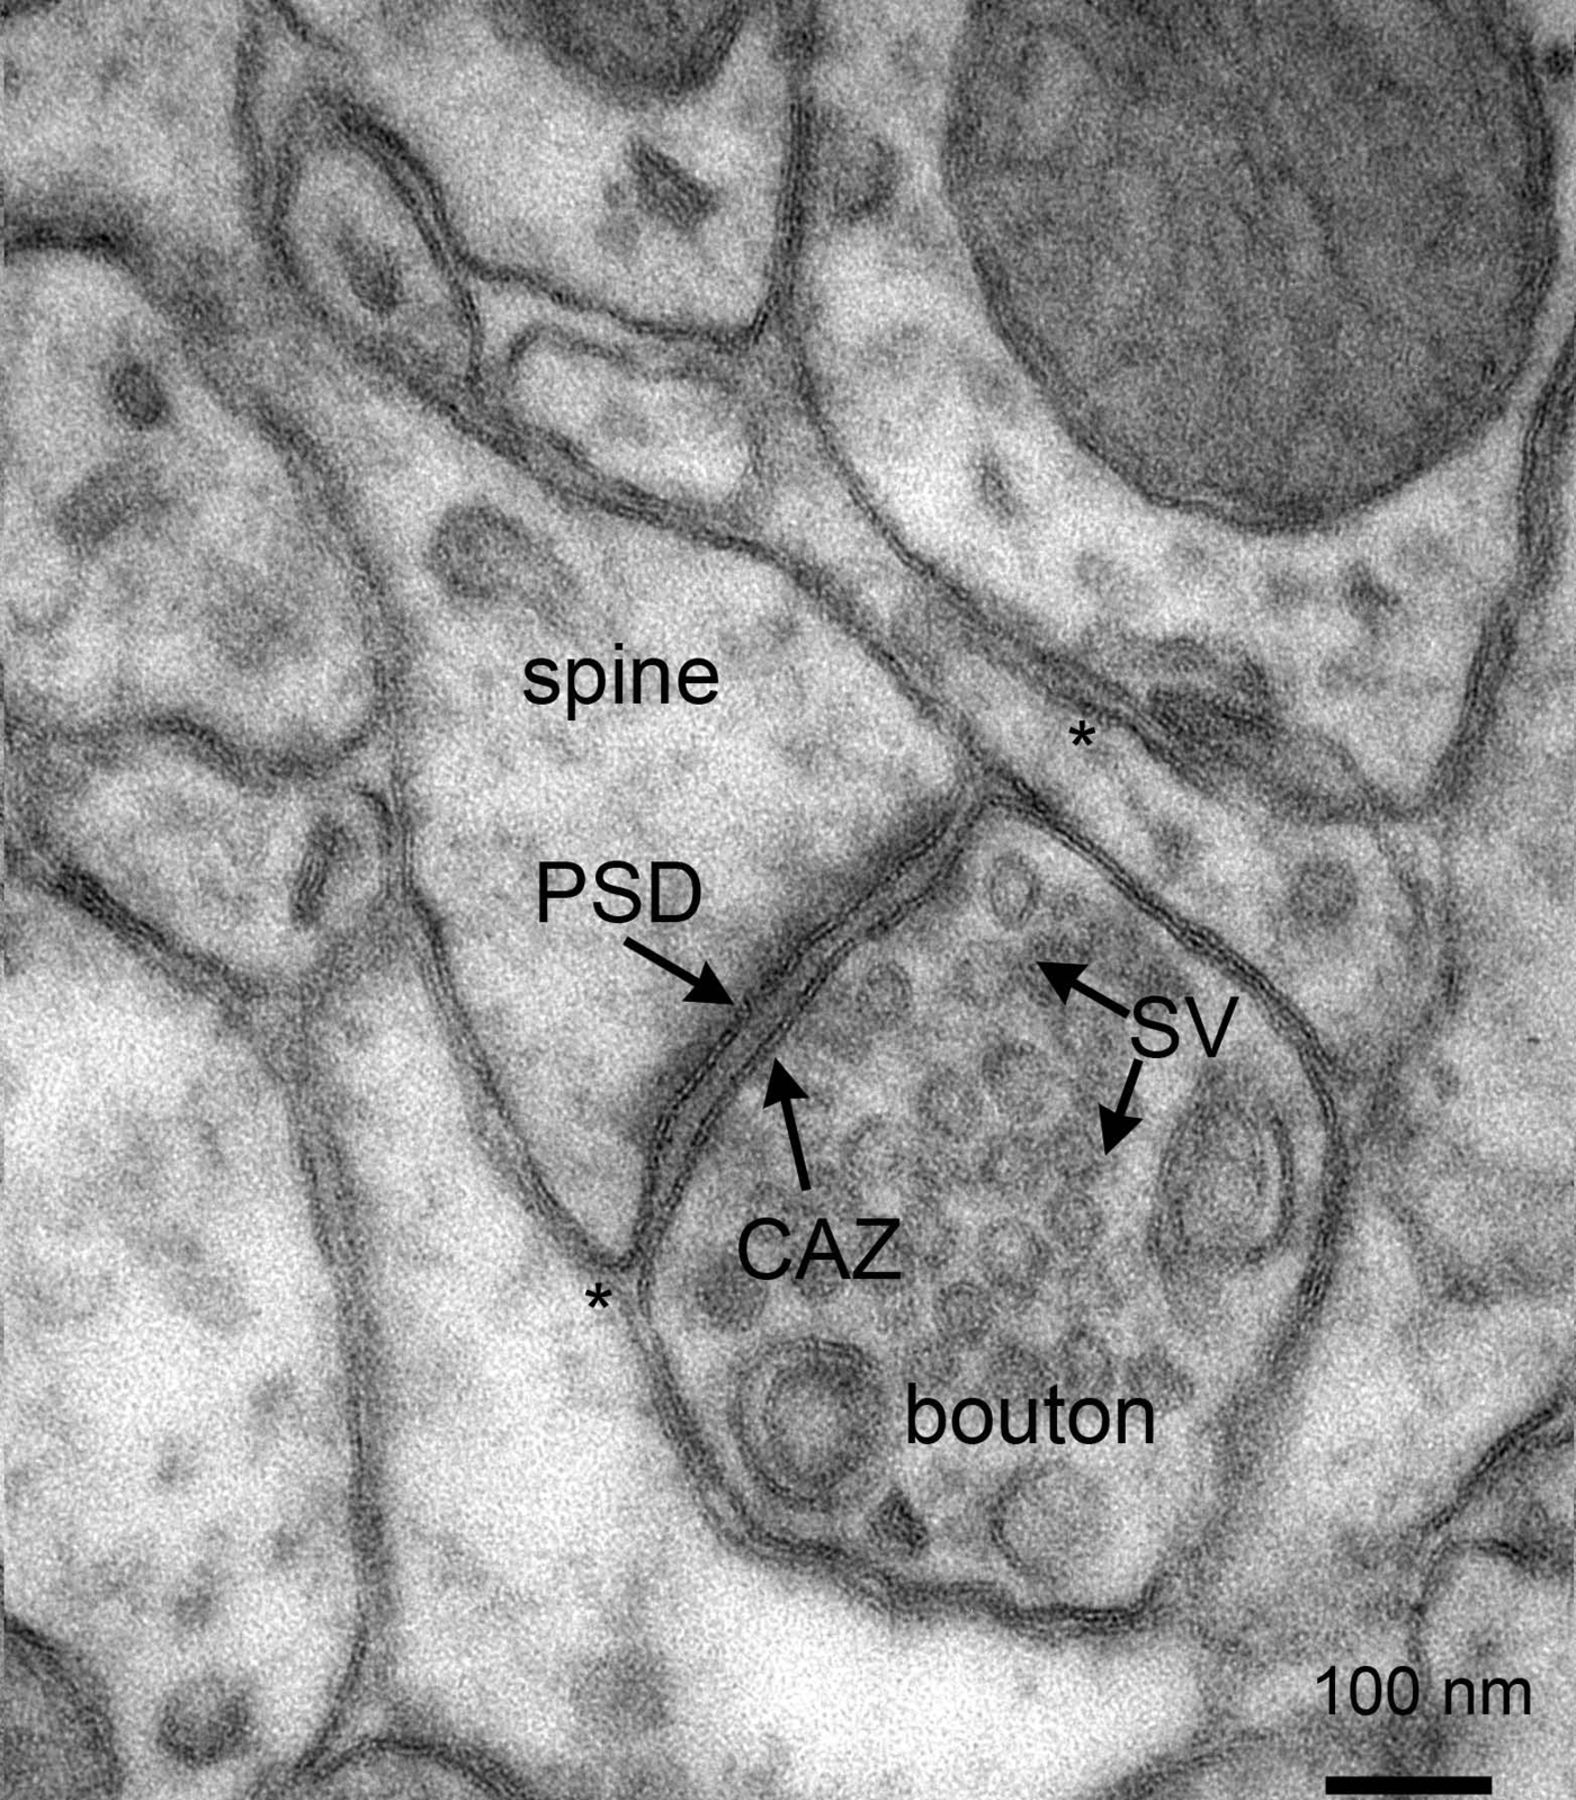
\includegraphics[width=0.7\linewidth]{./figures/synapse/synapse_electronmicrograph} 

}

\caption{Electron micrograph of rat cortex showing multiple pre- and postsynaptic structures, as well as astrocytic endfeet (*) in close contact with synapses. Note the presence of numerous synaptic vesicles in the presynaptic boutons. CAZ, cytomatrix at the active zone; PSD, postsynaptic density; SV, synaptic vesicles. Scalebar: 100 nm. From \href{https://doi.org/10.1074/mcp.R115.051482}{Proteomics of the Synapse -- A Quantitative Approach to Neuronal Plasticity Daniela C. Dieterich, Michael R. Kreutz Molecular \& Cellular Proteomics February 1, 2016, First published on August 25, 2015, 15 (2) 368-381; DOI: 10.1074/mcp.R115.051482}}\label{fig:electronsynapse}
\end{figure}

There are two fundamentally different types of synapses:

\begin{itemize}
\tightlist
\item
  In a chemical synapse, electrical activity in the presynaptic neuron is converted (via the activation of voltage-gated calcium channels) into the release of a chemical called a neurotransmitter that binds to receptors located in the plasma membrane of the postsynaptic cell. The neurotransmitter may initiate an electrical response or a secondary messenger pathway that may either excite or inhibit the postsynaptic neuron. Chemical synapses can be classified according to the neurotransmitter released: glutamatergic (often excitatory), GABAergic (often inhibitory), cholinergic (e.g.~vertebrate neuromuscular junction), and adrenergic (releasing norepinephrine). Because of the complexity of receptor signal transduction, chemical synapses can have complex effects on the postsynaptic cell.
\item
  In an electrical synapse, the presynaptic and postsynaptic cell membranes are connected by special channels called gap junctions that are capable of passing an electric current, causing voltage changes in the presynaptic cell to induce voltage changes in the postsynaptic cell. The main advantage of an electrical synapse is the rapid transfer of signals from one cell to the next.
\end{itemize}

Synapses can be classified by the type of cellular structures serving as the pre- and post-synaptic components. The vast majority of synapses in the mammalian nervous system are classical axo-dendritic synapses (axon synapsing upon a dendrite), however, a variety of other arrangements exist. These include but are not limited to axo-axonic, dendro-dendritic, axo-secretory, somato-dendritic, dendro-somatic, and somato-somatic synapses.

The axon can synapse onto a dendrite, onto a cell body, or onto another axon or axon terminal, as well as into the bloodstream or diffusely into the adjacent nervous tissue.

The postsynaptic density (PSD) is a protein dense specialization attached to the postsynaptic membrane. PSDs were originally identified by electron microscopy as an electron-dense region at the membrane of a postsynaptic neuron. The PSD is in close apposition to the presynaptic active zone and ensures that receptors are in close proximity to presynaptic neurotransmitter release sites. PSDs vary in size and composition among brain regions and have been studied in great detail at glutamatergic synapses. Hundreds of proteins have been identified in the postsynaptic density including glutamate receptors, scaffold proteins, and many signaling molecules.

PSDs are sized on the order of 250 to 500 nanometres in diameter and 25 to 50 nanometres in thickness, depending on the activity state of the synapse. During synaptic plasticity, the total size of the PSD is increasing along with an increase in synaptic size and strength after inducing long-term potentiation at single synapses.

Many proteins in the PSD are involved in the regulation of synaptic function. Key among these, are postsynaptic density-95 (PSD95), neuroligin (a cellular adhesion molecule), NMDA receptors, AMPA receptors, calcium/calmodulin-dependent protein kinase II and actin. As protein detection technologies have increased in sensitivity, such as with improvements in mass spectrometry techniques, many more proteins have been found to be part of the PSD. Current estimates are that several hundred proteins are found at PSDs in different brain regions and during different states of development and synaptic activity. PSDs also contain cell adhesion molecules and a diverse set of other signaling proteins. Many of the PSD proteins contain PDZ domains.



\begin{figure}

{\centering 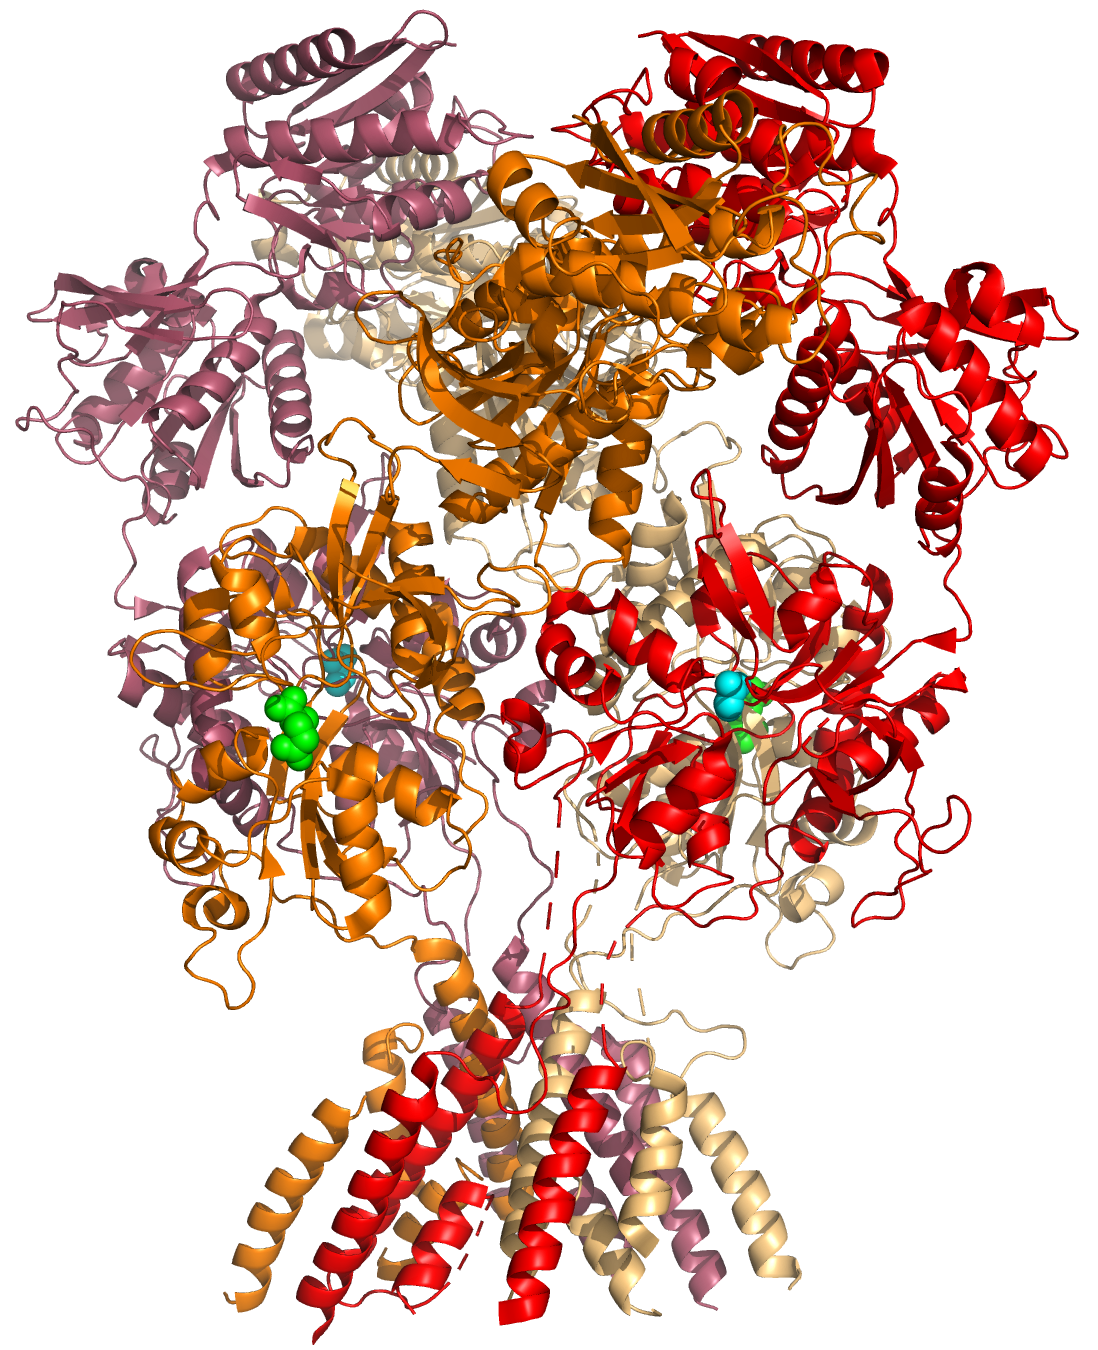
\includegraphics[width=0.7\linewidth]{./figures/synapse/NMDA_receptor} 

}

\caption{A cartoon representation of the atomic structure of the GluN1a/GluN2B N-Methyl-D-aspartate (NMDA) receptor subtype of the family of ionotropic glutamate receptors. The agonist glutamate (green spheres) is bound to the GluN2B subunit, the co-agonist glycine is bound to the GluN1A subunit. Data from \href{https://www.rcsb.org/structure/4PE5}{PDB 4PE5}, rendered with open source molecular visualization tool \href{https://pymol.org/2/}{PyMol}.}\label{fig:nmdar}
\end{figure}

The PSD has been proposed to concentrate and organize neurotransmitter receptors in the synaptic cleft. The PSD also serves as a signaling apparatus. For instance kinases and phosphatases in the PSD are activated and released from the PSD to change the activity of proteins located in the spine or are transported to the nucleus to affect protein synthesis. Some of the features of the PSD are similar to the neuromuscular junction and other cellular junctions, as the PSD has been modeled as a specialized cellular junction that allows for rapid, asymmetrical signaling.



\begin{figure}

{\centering 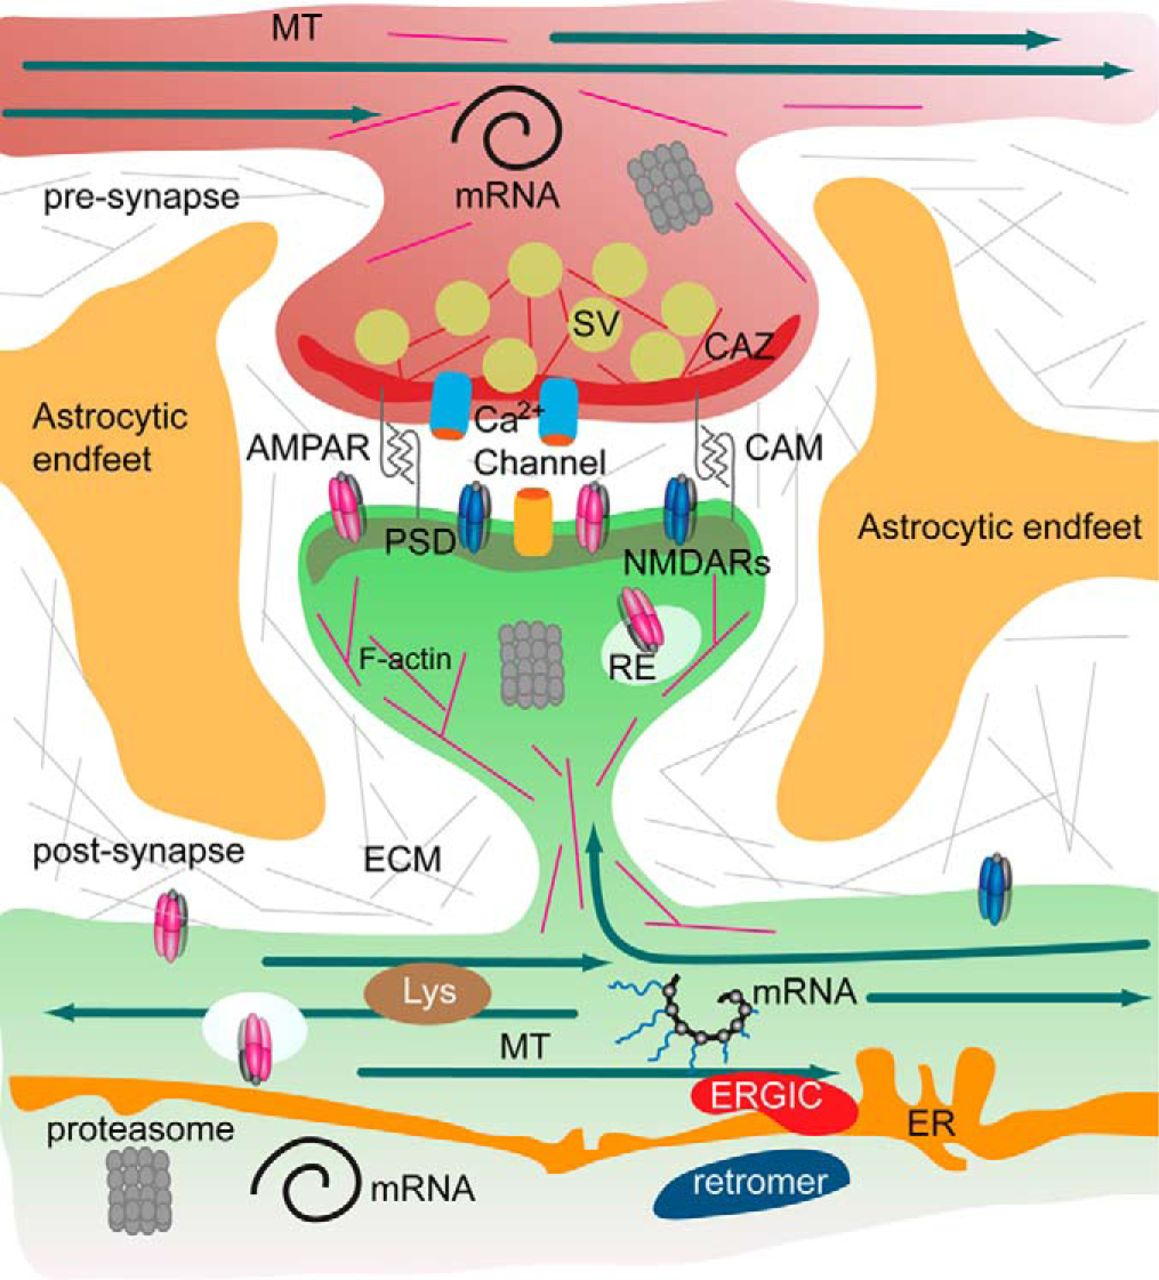
\includegraphics[width=0.7\linewidth]{./figures/synapse/synapse_diagram} 

}

\caption{The tetrapartite synapse of principal neurons in the forebrain, consisting of the pre- and postsynaptic compartment, astrocytic endfeet, and the extracellular matrix has a tightly regulated protein composition. A microsceretory system is present in synapses and dendrites that allows for translation of mRNA, local synthesis of, processing and insertion of transmembrane proteins. Hence the turnover of the synaptic protein machinery is controlled by local and somatic de novo protein synthesis, protein degradation by the ubiquitin proteasome system, lysosomes and autophagosomes. In addition, the association of proteins with pre- and postsynaptic compartments is highly dynamic. Molecular machineries and organelles for proteostasis are shared between synapses in dendritic segments. Proteins are transported in and out of the synapse as well as by diffusion of transmembrane proteins. These processes govern the activity-dependent assembly of the pre- and postsynaptic scaffold and the synaptic surface expression of receptors, calcium channels and cell adhesion molecules. Abbreviations: CAM, cell adhesion molecules; CAZ, cytomatrix at the active zone; ECM, extracellular matrix; ER, endoplasmatic reticulum; ERGIC, endoplasmatic reticulum Golgi intermediate compartment; MT, microtubules; PSD, postsynaptic density; RE, recycling endosomes; Lys, lysomes; SV, synaptic vesicle. From \href{https://doi.org/10.1074/mcp.R115.051482}{Proteomics of the Synapse -- A Quantitative Approach to Neuronal Plasticity Daniela C. Dieterich, Michael R. Kreutz Molecular \& Cellular Proteomics February 1, 2016, First published on August 25, 2015, 15 (2) 368-381; DOI: 10.1074/mcp.R115.051482}}\label{fig:synapsediagram}
\end{figure}

The adult human brain is estimated to contain from 10\textsuperscript{14} to 5 × 10\textsuperscript{14} (100--500 trillion) synapses. Every cubic millimeter of cerebral cortex contains roughly a billion (10\textsuperscript{9}) of them. The number of synapses in the human cerebral cortex has separately been estimated at 0.15 quadrillion (150 trillion)

It is widely accepted that the synapse plays a role in the formation of memory. As neurotransmitters activate receptors across the synaptic cleft, the connection between the two neurons is strengthened when both neurons are active at the same time, as a result of the receptor's signaling mechanisms. The strength of two connected neural pathways is thought to result in the storage of information, resulting in memory. This process of synaptic strengthening is known as long-term potentiation.

Synaptic transmission can be changed by previous activity. These changes are called synaptic plasticity and may result in either a decrease in the efficacy of the synapse, called depression, or an increase in efficacy, called potentiation. These changes can either be long-term or short-term. Forms of short-term plasticity include synaptic fatigue or depression and synaptic augmentation. Forms of long-term plasticity include long-term depression and long-term potentiation. Synaptic plasticity can be either homosynaptic (occurring at a single synapse) or heterosynaptic (occurring at multiple synapses).

By altering the release of neurotransmitters, the plasticity of synapses can be controlled in the presynaptic cell. The postsynaptic cell can be regulated by altering the function and number of its receptors. Changes in postsynaptic signaling are most commonly associated with a N-methyl-D-aspartic acid receptor (NMDAR)-dependent long-term potentiation (LTP) and long-term depression (LTD) due to the influx of calcium into the post-synaptic cell, which are the most analyzed forms of plasticity at excitatory synapses.

A neurotransmitter can influence the function of a neuron through a remarkable number of mechanisms. In its direct actions in influencing a neuron's electrical excitability, however, a neurotransmitter acts in only one of two ways: excitatory or inhibitory. A neurotransmitter influences trans-membrane ion flow either to increase (excitatory) or to decrease (inhibitory) the probability that the cell with which it comes in contact will produce an action potential. Thus, despite the wide variety of synapses, they all convey messages of only these two types, and they are labeled as such. Type I synapses are excitatory in their actions, whereas type II synapses are inhibitory. Each type has a different appearance and is located on different parts of the neurons under its influence.

Type I (excitatory) synapses are typically located on the shafts or the spines of dendrites, whereas type II (inhibitory) synapses are typically located on a cell body. In addition, Type I synapses have round synaptic vesicles, whereas the vesicles of type II synapses are flattened. The material on the presynaptic and post-synaptic membranes is denser in a Type I synapse than it is in a type II, and the type I synaptic cleft is wider. Finally, the active zone on a Type I synapse is larger than that on a Type II synapse.

The different locations of type I and type II synapses divide a neuron into two zones: an excitatory dendritic tree and an inhibitory cell body. From an inhibitory perspective, excitation comes in over the dendrites and spreads to the axon hillock to trigger an action potential. If the message is to be stopped, it is best stopped by applying inhibition on the cell body, close to the axon hillock where the action potential originates.

Here is a summary of the sequence of events that take place in synaptic transmission from a presynaptic neuron to a postsynaptic cell. Each step is explained in more detail below. Note that with the exception of the final step, the entire process may run only a few hundred microseconds, in the fastest synapses.

\begin{itemize}
\tightlist
\item
  The process begins with an action potential traveling along the membrane of the presynaptic cell, until it reaches the synapse.
\item
  The electrical depolarization of the membrane at the synapse causes channels to open that are permeable to calcium ions.
\item
  Calcium ions flow through the presynaptic membrane, rapidly increasing the calcium concentration in the interior.
\item
  The high calcium concentration activates a set of calcium-sensitive proteins attached to vesicles that contain a neurotransmitter chemical.
\item
  These proteins change shape, causing the membranes of some ``docked'' vesicles to fuse with the membrane of the presynaptic cell, thereby opening the vesicles and dumping their neurotransmitter contents into the synaptic cleft, the narrow space between the membranes of the pre- and postsynaptic cells.
\item
  The neurotransmitter diffuses within the cleft. Some of it escapes, but some of it binds to chemical receptor molecules located on the membrane of the postsynaptic cell.
\item
  The binding of neurotransmitter causes the receptor molecule to be activated.
\item
  Due to thermal vibration, the motion of atoms, vibrating about their equilibrium positions in a crystalline solid, neurotransmitter molecules eventually break loose from the receptors and drift away.
\item
  The neurotransmitter is either reabsorbed by the presynaptic cell, and then repackaged for future release, or else it is broken down metabolically.
\end{itemize}

In general, if an excitatory synapse is strong enough, an action potential in the presynaptic neuron will trigger an action potential in the postsynaptic cell. In many cases the excitatory postsynaptic potential (EPSP) will not reach the threshold for eliciting an action potential. When action potentials from multiple presynaptic neurons fire simultaneously, or if a single presynaptic neuron fires at a high enough frequency, the EPSPs can overlap and summate. If enough EPSPs overlap, the summated EPSP can reach the threshold for initiating an action potential. This process is known as summation.

On the other hand, a presynaptic neuron releasing an inhibitory neurotransmitter, such as GABA, can cause an inhibitory postsynaptic potential (IPSP) in the postsynaptic neuron, moving the membrane potential farther away from the threshold, decreasing its excitability and making it more difficult for the neuron to initiate an action potential. If an IPSP overlaps with an EPSP, the IPSP can in many cases prevent the neuron from firing an action potential. In this way, the output of a neuron may depend on the input of many different neurons, each of which may have a different degree of influence, depending on the strength and type of synapse with that neuron. \href{https://en.wikipedia.org/wiki/John_Eccles_(neurophysiologist)}{John Carew Eccles} performed some of the important early experiments on synaptic integration, for which he received the Nobel Prize for Physiology or Medicine in 1963.

Understanding the effects of drugs on neurotransmitters comprises a significant portion of research initiatives in the field of neuroscience. Most neuroscientists involved in this field of research believe that such efforts may further advance our understanding of the circuits responsible for various neurological diseases and disorders, as well as ways to effectively treat and someday possibly prevent or cure such illnesses.

\hypertarget{neurotransmitters}{%
\subsection{Neurotransmitters}\label{neurotransmitters}}

Neurotransmitters are endogenous chemicals that enable neurotransmission. It is a type of chemical messenger which transmits signals across a chemical synapse, such as a neuromuscular junction, from one neuron (nerve cell) to another ``target'' neuron, muscle cell, or gland cell. Neurotransmitters are released from synaptic vesicles in synapses into the synaptic cleft, where they are received by neurotransmitter receptors on the target cells. Many neurotransmitters are synthesized from simple and plentiful precursors such as amino acids, which are readily available from the diet and only require a small number of biosynthetic steps for conversion. Neurotransmitters play a major role in shaping everyday life and functions. Their exact numbers are unknown, but more than 200 unique chemical messengers have been identified.

Neurotransmitters are stored in synaptic vesicles, clustered close to the cell membrane at the axon terminal of the presynaptic neuron. Neurotransmitters are released into and diffuse across the synaptic cleft, where they bind to specific receptors on the membrane of the postsynaptic neuron.

Neurotransmitter action is terminated in three different ways:

\begin{itemize}
\tightlist
\item
  Diffusion -- the neurotransmitter detaches from receptor, drifting out of the synaptic cleft, here it becomes absorbed by glial cells.
\item
  Enzyme degradation -- special chemicals called enzymes break it down. Usually, astrocytes absorb the excess neurotransmitters and pass them on to enzymes or pump them directly into the presynaptic neuron.
\item
  Reuptake -- re-absorption of a neurotransmitter into the neuron. Transporters, or membrane transport proteins, pump neurotransmitters from the synaptic cleft back into axon terminals (the presynaptic neuron) where they are stored.
\end{itemize}

For example, choline is taken up and recycled by the pre-synaptic neuron to synthesize more ACh. Other neurotransmitters such as dopamine are able to diffuse away from their targeted synaptic junctions and are eliminated from the body via the kidneys, or destroyed in the liver. Each neurotransmitter has very specific degradation pathways at regulatory points, which may be targeted by the body's regulatory system or by recreational drugs.

Until the early 20th century, scientists assumed that the majority of synaptic communication in the brain was electrical. But in 1921 German pharmacologist \href{https://en.wikipedia.org/wiki/Otto_Loewi}{Otto Loewi} (1873--1961) demonstrated that neurons can communicate by releasing chemicals. Some neurons do, however, communicate via electrical synapses through the use of gap junctions, which allow specific ions to pass directly from one cell to another.

The anatomical localization of neurotransmitters is typically determined using immunocytochemical techniques, which identify the location of either the transmitter substances themselves, or of the enzymes that are involved in their synthesis. Immunocytochemical techniques have also revealed that many transmitters, particularly the neuropeptides, are co-localized, that is, one neuron may release more than one transmitter from its synaptic terminal. Various techniques have been used to identify neurotransmitters throughout the central nervous system.

Single ions (such as synaptically released zinc) are also considered neurotransmitters by some, as well as some gaseous molecules such as nitric oxide (NO), carbon monoxide (CO), and hydrogen sulfide (H\textsubscript{2}S).

The most prevalent transmitter is glutamate, which is excitatory at well over 90\% of the synapses in the human brain. The next most prevalent is Gamma-Aminobutyric Acid, or GABA, which is inhibitory at more than 90\% of the synapses that do not use glutamate. Although other transmitters are used in fewer synapses, they may be very important functionally: the great majority of psychoactive drugs exert their effects by altering the actions of some neurotransmitter systems, often acting through transmitters other than glutamate or GABA. Addictive drugs such as cocaine and amphetamines exert their effects primarily on the dopamine system. The addictive opiate drugs exert their effects primarily as functional analogs of opioid peptides, which, in turn, regulate dopamine levels.

\hypertarget{modulatory-neurotransmitter-systems}{%
\subsection{Modulatory Neurotransmitter Systems}\label{modulatory-neurotransmitter-systems}}

Neurons expressing certain types of neurotransmitters sometimes form distinct systems, where activation of the system acts in a modulatory fashion on a large number of neurons in large volumes of the brain. Such modulatory neurotransmitter systems include the noradrenaline (norepinephrine) system, the dopamine system, the serotonin system, and the cholinergic system, among others. Neuromodulatory neurotransmitters typically bind to metabotropic, G-protein coupled receptors to initiate a second messenger signaling cascade that induces a broad, long-lasting signal. This modulation can last for hundreds of milliseconds to several minutes. Some of the effects of neuromodulators include: altering the intrinsic firing activity, increasing or decreasing voltage-dependent currents, changing synaptic efficacy, increasing bursting activity and reconfiguring of synaptic connectivity.

\hypertarget{neurotransmitter-receptors}{%
\subsection{Neurotransmitter Receptors}\label{neurotransmitter-receptors}}

There are two major types of neurotransmitter receptors: ionotropic and metabotropic. Ionotropic means that ions can pass through the receptor, whereas metabotropic means that a second messenger inside the cell relays the message (i.e.~metabotropic receptors do not have channels). Metabotropic receptors are G-protein-coupled receptors (GPCRs). Ionotropic receptors are also called ligand-gated ion channels. Conversely, GPCRs are neither excitatory nor inhibitory. Rather, they can have a broad number of functions such as modulating the actions of excitatory and inhibitory ion channels or triggering a signalling cascade that releases calcium from stores inside the cell.

\hypertarget{ionotropic-receptors-neurotransmitter-gated-ion-channels}{%
\subsection{Ionotropic Receptors: Neurotransmitter-Gated Ion Channels}\label{ionotropic-receptors-neurotransmitter-gated-ion-channels}}

Ligand-gated ion channels (LGICs) are one type of ionotropic receptor or channel-linked receptor. They are a group of transmembrane ion channels that are opened or closed in response to the binding of a chemical messenger (i.e., a ligand), such as a neurotransmitter.



\begin{figure}

{\centering 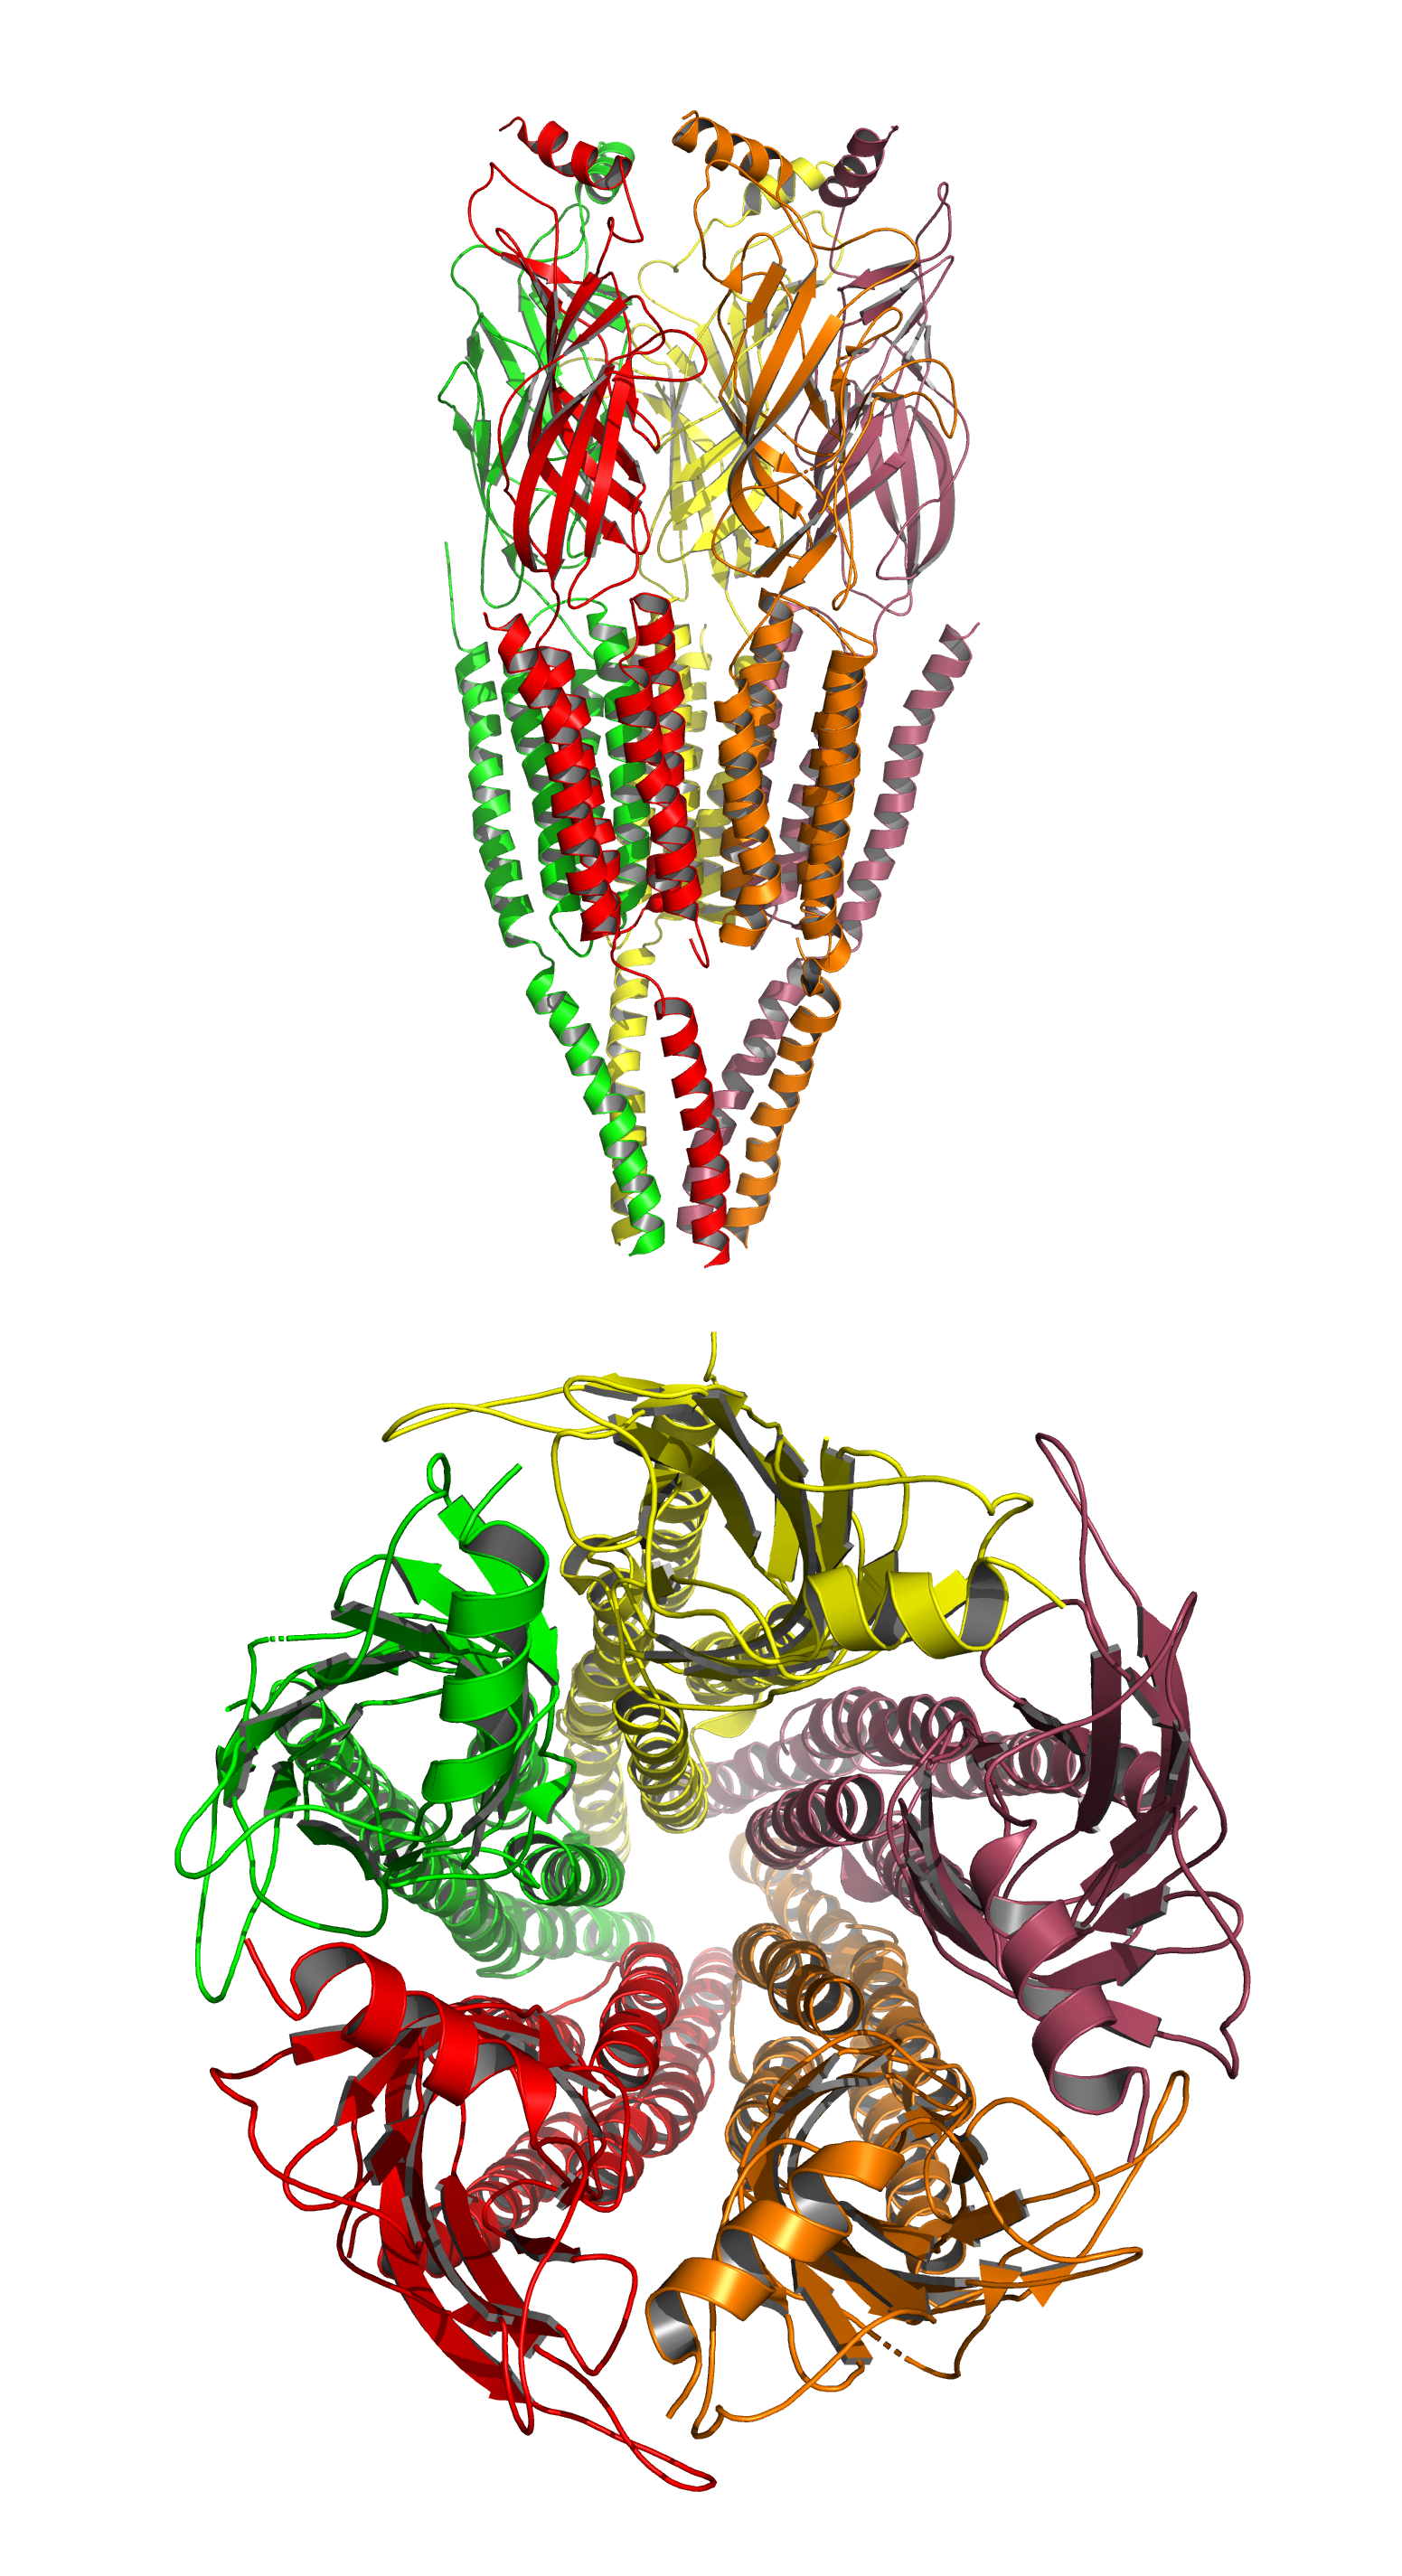
\includegraphics[width=0.7\linewidth]{./figures/synapse/nAch_receptor} 

}

\caption{A cartoon representation of the atomic structure of the the nicotinic acetylcholine receptor from the electric ray \emph{Torpedo marmorata} at 4Å resolution. Data from \href{https://www.rcsb.org/structure/2BG9}{PDB 2BG9}, rendered with open source molecular visualization tool \href{https://pymol.org/2/}{PyMol}.}\label{fig:achr}
\end{figure}

The binding site of endogenous ligands on LGICs protein complexes are normally located on a different portion of the protein (an allosteric binding site) compared to where the ion conduction pore is located. The direct link between ligand binding and opening or closing of the ion channel, which is characteristic of ligand-gated ion channels, is contrasted with the indirect function of metabotropic receptors, which use second messengers. LGICs are also different from voltage-gated ion channels (which open and close depending on membrane potential), and stretch-activated ion channels (which open and close depending on mechanical deformation of the cell membrane).

\hypertarget{metabotropic-receptors-g-protein-coupled-receptors}{%
\subsection{Metabotropic Receptors: G-Protein Coupled Receptors}\label{metabotropic-receptors-g-protein-coupled-receptors}}

GPCRs also known as seven-transmembrane domain receptors, 7TM receptors, heptahelical receptors, serpentine receptor comprise a large protein family of transmembrane receptors that sense molecules outside the cell and activate intracellular signal transduction pathways. GPCRs are found only in eukaryotes. The ligands that bind and activate these receptors include light-sensitive compounds, odors, pheromones, hormones, and neurotransmitters, and vary in size from small molecules to peptides to large proteins. G protein-coupled receptors are involved in many diseases, and are also the target of approximately 30\% of all modern medicinal drugs.

There are two principal signal transduction pathways involving the G protein-coupled receptors: the cAMP signal pathway and the phosphatidylinositol signal pathway. When a ligand binds to the GPCR it causes a conformational change in the GPCR, which allows it to act as a guanine nucleotide exchange factor (GEF). The GPCR can then activate an associated G-protein by exchanging its bound GDP for a GTP. The G-protein's α subunit, together with the bound GTP, can then dissociate from the β and γ subunits to further affect intracellular signaling proteins or target functional proteins directly depending on the α subunit type (G\textsubscript{αs}, G\textsubscript{αi/o}, G\textsubscript{αq/11}, G\textsubscript{α12/13}).

Neurotransmitter receptors are present on both postsynaptic neurons and presynaptic neurons with the former being used to receive neurotransmitters and the latter for the purpose of preventing further release of a given neurotransmitter. In addition to being found in neuron cells, neurotransmitter receptors are also found in various immune and muscle tissues. Many neurotransmitter receptors are categorized as a serpentine receptor or G protein-coupled receptor because they span the cell membrane not once, but seven times. Neurotransmitter receptors are known to become unresponsive to the type of neurotransmitter they receive when exposed for extended periods of time. This phenomenon is known as ligand-induced desensitization or downregulation.

The following are some major classes of neurotransmitter receptors:

\begin{itemize}
\tightlist
\item
  Adrenergic: α1A, α1b, α1c, α1d, α2a, α2b, α2c, α2d, β1, β2, β3
\item
  Dopaminergic: D1, D2, D3, D4, D5
\item
  GABAergic: GABA\textsubscript{A}, GABA\textsubscript{B1a}, GABA\textsubscript{B1δ}, GABA\textsubscript{B2}, GABA\textsubscript{C}
\item
  Glutamatergic: NMDA, AMPA, kainate, mGluR1, mGluR2, mGluR3, mGluR4, mGluR5, mGluR6, mGluR7
\item
  Histaminergic: H1, H2, H3
\item
  Cholinergic: Muscarinic: M1, M2, M3, M4, M5; Nicotinic: muscle, neuronal (α-bungarotoxin-insensitive), neuronal (α-bungarotoxin-sensitive)
\item
  Opioid: μ, δ1, δ2, κ
\item
  Serotonergic: 5-HT1A, 5-HT1B, 5-HT1D, 5-HT1E, 5-HT1F, 5-HT2A, 5-HT2B, 5-HT2C, 5-HT3, 5-HT4, 5-HT5, 5-HT6, 5-HT7
\item
  Glycinergic: Glycine
\end{itemize}

Drugs can influence behavior by altering neurotransmitter activity. For instance, drugs can decrease the rate of synthesis of neurotransmitters by affecting the synthetic enzyme(s) for that neurotransmitter. When neurotransmitter synthesis is blocked, the amount of neurotransmitters available for release becomes substantially lower, resulting in a decrease in neurotransmitter activity. Some drugs block or stimulate the release of specific neurotransmitters. Alternatively, drugs can prevent neurotransmitter storage in synaptic vesicles by causing the synaptic vesicle membranes to leak. Drugs that prevent a neurotransmitter from binding to its receptor are called receptor antagonists. For example, drugs used to treat patients with schizophrenia such as haloperidol, chlorpromazine, and clozapine are antagonists at receptors in the brain for dopamine. Other drugs act by binding to a receptor and mimicking the normal neurotransmitter. Such drugs are called receptor agonists. An example of a receptor agonist is morphine, an opiate that mimics effects of the endogenous neurotransmitter β-endorphin to relieve pain. Other drugs interfere with the deactivation of a neurotransmitter after it has been released, thereby prolonging the action of a neurotransmitter. This can be accomplished by blocking re-uptake or inhibiting degradative enzymes. Lastly, drugs can also prevent an action potential from occurring, blocking neuronal activity throughout the central and peripheral nervous system.


